\documentclass{book}
\usepackage[a4paper,top=2.5cm,bottom=2.5cm,left=2.5cm,right=2.5cm]{geometry}
\usepackage{makeidx}
\usepackage{natbib}
\usepackage{graphicx}
\usepackage{multicol}
\usepackage{float}
\usepackage{listings}
\usepackage{color}
\usepackage{ifthen}
\usepackage[table]{xcolor}
\usepackage{textcomp}
\usepackage{alltt}
\usepackage{ifpdf}
\ifpdf
\usepackage[pdftex,
            pagebackref=true,
            colorlinks=true,
            linkcolor=blue,
            unicode
           ]{hyperref}
\else
\usepackage[ps2pdf,
            pagebackref=true,
            colorlinks=true,
            linkcolor=blue,
            unicode
           ]{hyperref}
\usepackage{pspicture}
\fi
\usepackage[utf8]{inputenc}
\usepackage[T2A]{fontenc}
\usepackage[russian]{babel}

\usepackage{mathptmx}
\usepackage[scaled=.90]{helvet}
\usepackage{courier}
\usepackage{sectsty}
\usepackage{amssymb}
\usepackage[titles]{tocloft}
\usepackage{doxygen}
\lstset{language=C++,inputencoding=utf8,basicstyle=\footnotesize,breaklines=true,breakatwhitespace=true,tabsize=10,numbers=left }
\makeindex
\setcounter{tocdepth}{3}
\renewcommand{\footrulewidth}{0.4pt}
\renewcommand{\familydefault}{\sfdefault}
\hfuzz=15pt
\setlength{\emergencystretch}{15pt}
\hbadness=750
\tolerance=750
\begin{document}
\hypersetup{pageanchor=false,citecolor=blue}
\begin{titlepage}
\vspace*{7cm}
\begin{center}
{\Large S\-M\-P\-L\-Sharp }\\
\vspace*{1cm}
{\large Создано системой Doxygen 1.8.3.1}\\
\vspace*{0.5cm}
{\small Пт 5 Апр 2013 18:24:17}\\
\end{center}
\end{titlepage}
\clearemptydoublepage
\pagenumbering{roman}
\tableofcontents
\clearemptydoublepage
\pagenumbering{arabic}
\hypersetup{pageanchor=true,citecolor=blue}
\chapter{Алфавитный указатель пространств имен}
\section{Пакеты}
Полный список документированных пакетов.\begin{DoxyCompactList}
\item\contentsline{section}{\hyperlink{namespace_s_m_p_l_sharp}{S\-M\-P\-L\-Sharp} }{\pageref{dd/d3b/namespace_s_m_p_l_sharp}}{}
\item\contentsline{section}{\hyperlink{namespace_s_m_p_l_sharp_1_1_objects}{S\-M\-P\-L\-Sharp.\-Objects} }{\pageref{d9/d75/namespace_s_m_p_l_sharp_1_1_objects}}{}
\item\contentsline{section}{\hyperlink{namespace_s_m_p_l_sharp_1_1_utils}{S\-M\-P\-L\-Sharp.\-Utils} }{\pageref{d4/de6/namespace_s_m_p_l_sharp_1_1_utils}}{}
\end{DoxyCompactList}

\chapter{Иерархический список классов}
\section{Иерархия классов}
Иерархия классов.\begin{DoxyCompactList}
\item \contentsline{section}{S\-M\-P\-L\-Sharp.\-Objects.\-Smpl\-Multi\-Device.\-Ambary}{\pageref{d1/df4/struct_s_m_p_l_sharp_1_1_objects_1_1_smpl_multi_device_1_1_ambary}}{}
\item Event\-Args\begin{DoxyCompactList}
\item \contentsline{section}{S\-M\-P\-L\-Sharp.\-Event\-Caused\-Event\-Args}{\pageref{d0/dff/class_s_m_p_l_sharp_1_1_event_caused_event_args}}{}
\end{DoxyCompactList}
\item \contentsline{section}{S\-M\-P\-L\-Sharp.\-Objects.\-Smpl\-Device}{\pageref{d7/d39/class_s_m_p_l_sharp_1_1_objects_1_1_smpl_device}}{}
\item \contentsline{section}{S\-M\-P\-L\-Sharp.\-Objects.\-Smpl\-Event}{\pageref{de/d57/class_s_m_p_l_sharp_1_1_objects_1_1_smpl_event}}{}
\item \contentsline{section}{S\-M\-P\-L\-Sharp.\-Smpl\-Model}{\pageref{df/d34/class_s_m_p_l_sharp_1_1_smpl_model}}{}
\item \contentsline{section}{S\-M\-P\-L\-Sharp.\-Objects.\-Smpl\-Multi\-Device}{\pageref{d8/d23/class_s_m_p_l_sharp_1_1_objects_1_1_smpl_multi_device}}{}
\item \contentsline{section}{S\-M\-P\-L\-Sharp.\-Objects.\-Smpl\-Queue}{\pageref{d3/ded/class_s_m_p_l_sharp_1_1_objects_1_1_smpl_queue}}{}
\item \contentsline{section}{S\-M\-P\-L\-Sharp.\-Objects.\-Smpl\-Queue\-Element}{\pageref{d3/d48/class_s_m_p_l_sharp_1_1_objects_1_1_smpl_queue_element}}{}
\item \contentsline{section}{S\-M\-P\-L\-Sharp.\-Utils.\-Smpl\-Random\-Generator}{\pageref{d0/d33/class_s_m_p_l_sharp_1_1_utils_1_1_smpl_random_generator}}{}
\item \contentsline{section}{S\-M\-P\-L\-Sharp.\-Utils.\-Smpl\-R\-Device\-Statisic}{\pageref{d7/d3b/class_s_m_p_l_sharp_1_1_utils_1_1_smpl_r_device_statisic}}{}
\begin{DoxyCompactList}
\item \contentsline{section}{S\-M\-P\-L\-Sharp.\-Utils.\-Smpl\-R\-Multi\-Device\-Statisic}{\pageref{de/d2e/class_s_m_p_l_sharp_1_1_utils_1_1_smpl_r_multi_device_statisic}}{}
\end{DoxyCompactList}
\item \contentsline{section}{S\-M\-P\-L\-Sharp.\-Utils.\-Smpl\-Reporter}{\pageref{d2/d18/class_s_m_p_l_sharp_1_1_utils_1_1_smpl_reporter}}{}
\item \contentsline{section}{S\-M\-P\-L\-Sharp.\-Utils.\-Smpl\-R\-Queue\-Statisic}{\pageref{de/de9/class_s_m_p_l_sharp_1_1_utils_1_1_smpl_r_queue_statisic}}{}
\end{DoxyCompactList}

\chapter{Алфавитный указатель классов}
\section{Классы}
Классы с их кратким описанием.\begin{DoxyCompactList}
\item\contentsline{section}{\hyperlink{struct_s_m_p_l_sharp_1_1_objects_1_1_smpl_multi_device_1_1_ambary}{S\-M\-P\-L\-Sharp.\-Objects.\-Smpl\-Multi\-Device.\-Ambary} \\*Канал прибора }{\pageref{d1/df4/struct_s_m_p_l_sharp_1_1_objects_1_1_smpl_multi_device_1_1_ambary}}{}
\item\contentsline{section}{\hyperlink{class_s_m_p_l_sharp_1_1_event_caused_event_args}{S\-M\-P\-L\-Sharp.\-Event\-Caused\-Event\-Args} \\*Event when model's event is caused }{\pageref{d0/dff/class_s_m_p_l_sharp_1_1_event_caused_event_args}}{}
\item\contentsline{section}{\hyperlink{class_s_m_p_l_sharp_1_1_objects_1_1_smpl_device}{S\-M\-P\-L\-Sharp.\-Objects.\-Smpl\-Device} \\*Equipment or facility Typically represents some work-\/performing resource of system being modeled The Interconnection of facilities is not explicit, but can be determined by the model’s routing of tokens between facilities }{\pageref{d7/d39/class_s_m_p_l_sharp_1_1_objects_1_1_smpl_device}}{}
\item\contentsline{section}{\hyperlink{class_s_m_p_l_sharp_1_1_objects_1_1_smpl_event}{S\-M\-P\-L\-Sharp.\-Objects.\-Smpl\-Event} \\*Model's event A change of state of any system entity, active or passive Can be, for example, Arrival of task or Computing completion }{\pageref{de/d57/class_s_m_p_l_sharp_1_1_objects_1_1_smpl_event}}{}
\item\contentsline{section}{\hyperlink{class_s_m_p_l_sharp_1_1_smpl_model}{S\-M\-P\-L\-Sharp.\-Smpl\-Model} \\*Simulation model. Provides set of function for building event-\/based, discrete-\/event simulation model }{\pageref{df/d34/class_s_m_p_l_sharp_1_1_smpl_model}}{}
\item\contentsline{section}{\hyperlink{class_s_m_p_l_sharp_1_1_objects_1_1_smpl_multi_device}{S\-M\-P\-L\-Sharp.\-Objects.\-Smpl\-Multi\-Device} \\*Equipment or facility Typically represents some work-\/performing resource of system being modeled The Interconnection of facilities is not explicit, but can be determined by the model’s routing of tokens between facilities }{\pageref{d8/d23/class_s_m_p_l_sharp_1_1_objects_1_1_smpl_multi_device}}{}
\item\contentsline{section}{\hyperlink{class_s_m_p_l_sharp_1_1_objects_1_1_smpl_queue}{S\-M\-P\-L\-Sharp.\-Objects.\-Smpl\-Queue} \\*Очередь. Represents place where tokens are waiting when equipment is busy }{\pageref{d3/ded/class_s_m_p_l_sharp_1_1_objects_1_1_smpl_queue}}{}
\item\contentsline{section}{\hyperlink{class_s_m_p_l_sharp_1_1_objects_1_1_smpl_queue_element}{S\-M\-P\-L\-Sharp.\-Objects.\-Smpl\-Queue\-Element} \\*Элемент очереди }{\pageref{d3/d48/class_s_m_p_l_sharp_1_1_objects_1_1_smpl_queue_element}}{}
\item\contentsline{section}{\hyperlink{class_s_m_p_l_sharp_1_1_utils_1_1_smpl_random_generator}{S\-M\-P\-L\-Sharp.\-Utils.\-Smpl\-Random\-Generator} \\*Генератор случайных чисел }{\pageref{d0/d33/class_s_m_p_l_sharp_1_1_utils_1_1_smpl_random_generator}}{}
\item\contentsline{section}{\hyperlink{class_s_m_p_l_sharp_1_1_utils_1_1_smpl_r_device_statisic}{S\-M\-P\-L\-Sharp.\-Utils.\-Smpl\-R\-Device\-Statisic} \\*Статистика по прибору }{\pageref{d7/d3b/class_s_m_p_l_sharp_1_1_utils_1_1_smpl_r_device_statisic}}{}
\item\contentsline{section}{\hyperlink{class_s_m_p_l_sharp_1_1_utils_1_1_smpl_reporter}{S\-M\-P\-L\-Sharp.\-Utils.\-Smpl\-Reporter} \\*Give model statistic }{\pageref{d2/d18/class_s_m_p_l_sharp_1_1_utils_1_1_smpl_reporter}}{}
\item\contentsline{section}{\hyperlink{class_s_m_p_l_sharp_1_1_utils_1_1_smpl_r_multi_device_statisic}{S\-M\-P\-L\-Sharp.\-Utils.\-Smpl\-R\-Multi\-Device\-Statisic} \\*Статистика по многоканальному прибору }{\pageref{de/d2e/class_s_m_p_l_sharp_1_1_utils_1_1_smpl_r_multi_device_statisic}}{}
\item\contentsline{section}{\hyperlink{class_s_m_p_l_sharp_1_1_utils_1_1_smpl_r_queue_statisic}{S\-M\-P\-L\-Sharp.\-Utils.\-Smpl\-R\-Queue\-Statisic} \\*Статистика по очереди }{\pageref{de/de9/class_s_m_p_l_sharp_1_1_utils_1_1_smpl_r_queue_statisic}}{}
\end{DoxyCompactList}

\chapter{Пространства имен}
\hypertarget{namespace_s_m_p_l_sharp}{\section{Пакет S\-M\-P\-L\-Sharp}
\label{dd/d3b/namespace_s_m_p_l_sharp}\index{S\-M\-P\-L\-Sharp@{S\-M\-P\-L\-Sharp}}
}
\subsection*{Пространства имен}
\begin{DoxyCompactItemize}
\item 
package \hyperlink{namespace_s_m_p_l_sharp_1_1_objects}{Objects}
\item 
package \hyperlink{namespace_s_m_p_l_sharp_1_1_utils}{Utils}
\end{DoxyCompactItemize}
\subsection*{Классы}
\begin{DoxyCompactItemize}
\item 
class \hyperlink{class_s_m_p_l_sharp_1_1_smpl_model}{Smpl\-Model}
\begin{DoxyCompactList}\small\item\em Simulation model. Provides set of function for building event-\/based, discrete-\/event simulation model \end{DoxyCompactList}\item 
class \hyperlink{class_s_m_p_l_sharp_1_1_event_caused_event_args}{Event\-Caused\-Event\-Args}
\begin{DoxyCompactList}\small\item\em Event when model's event is caused \end{DoxyCompactList}\end{DoxyCompactItemize}
\subsection*{Функции}
\begin{DoxyCompactItemize}
\item 
delegate void \hyperlink{namespace_s_m_p_l_sharp_a33fb2904b12541599362cddd40c71357}{Event\-Caused\-Handler} (object o, \hyperlink{class_s_m_p_l_sharp_1_1_event_caused_event_args}{Event\-Caused\-Event\-Args} e)
\begin{DoxyCompactList}\small\item\em Delegate for Event\-Caused \end{DoxyCompactList}\end{DoxyCompactItemize}


\subsection{Функции}
\hypertarget{namespace_s_m_p_l_sharp_a33fb2904b12541599362cddd40c71357}{\index{S\-M\-P\-L\-Sharp@{S\-M\-P\-L\-Sharp}!Event\-Caused\-Handler@{Event\-Caused\-Handler}}
\index{Event\-Caused\-Handler@{Event\-Caused\-Handler}!SMPLSharp@{S\-M\-P\-L\-Sharp}}
\subsubsection[{Event\-Caused\-Handler}]{\setlength{\rightskip}{0pt plus 5cm}delegate void S\-M\-P\-L\-Sharp.\-Event\-Caused\-Handler (
\begin{DoxyParamCaption}
\item[{object}]{o, }
\item[{Event\-Caused\-Event\-Args}]{e}
\end{DoxyParamCaption}
)}}\label{dd/d3b/namespace_s_m_p_l_sharp_a33fb2904b12541599362cddd40c71357}


Delegate for Event\-Caused 


\begin{DoxyParams}{Аргументы}
{\em o} & \\
\hline
{\em e} & \\
\hline
\end{DoxyParams}

\hypertarget{namespace_s_m_p_l_sharp_1_1_objects}{\section{Пакет S\-M\-P\-L\-Sharp.\-Objects}
\label{d9/d75/namespace_s_m_p_l_sharp_1_1_objects}\index{S\-M\-P\-L\-Sharp.\-Objects@{S\-M\-P\-L\-Sharp.\-Objects}}
}
\subsection*{Классы}
\begin{DoxyCompactItemize}
\item 
class \hyperlink{class_s_m_p_l_sharp_1_1_objects_1_1_smpl_device}{Smpl\-Device}
\begin{DoxyCompactList}\small\item\em Equipment or facility Typically represents some work-\/performing resource of system being modeled The Interconnection of facilities is not explicit, but can be determined by the model’s routing of tokens between facilities \end{DoxyCompactList}\item 
class \hyperlink{class_s_m_p_l_sharp_1_1_objects_1_1_smpl_event}{Smpl\-Event}
\begin{DoxyCompactList}\small\item\em Model's event A change of state of any system entity, active or passive Can be, for example, Arrival of task or Computing completion \end{DoxyCompactList}\item 
class \hyperlink{class_s_m_p_l_sharp_1_1_objects_1_1_smpl_multi_device}{Smpl\-Multi\-Device}
\begin{DoxyCompactList}\small\item\em Equipment or facility Typically represents some work-\/performing resource of system being modeled The Interconnection of facilities is not explicit, but can be determined by the model’s routing of tokens between facilities \end{DoxyCompactList}\item 
class \hyperlink{class_s_m_p_l_sharp_1_1_objects_1_1_smpl_queue}{Smpl\-Queue}
\begin{DoxyCompactList}\small\item\em Очередь. Represents place where tokens are waiting when equipment is busy \end{DoxyCompactList}\item 
class \hyperlink{class_s_m_p_l_sharp_1_1_objects_1_1_smpl_queue_element}{Smpl\-Queue\-Element}
\begin{DoxyCompactList}\small\item\em Элемент очереди \end{DoxyCompactList}\end{DoxyCompactItemize}

\hypertarget{namespace_s_m_p_l_sharp_1_1_utils}{\section{Пакет S\-M\-P\-L\-Sharp.\-Utils}
\label{d4/de6/namespace_s_m_p_l_sharp_1_1_utils}\index{S\-M\-P\-L\-Sharp.\-Utils@{S\-M\-P\-L\-Sharp.\-Utils}}
}
\subsection*{Классы}
\begin{DoxyCompactItemize}
\item 
class \hyperlink{class_s_m_p_l_sharp_1_1_utils_1_1_smpl_random_generator}{Smpl\-Random\-Generator}
\begin{DoxyCompactList}\small\item\em Генератор случайных чисел \end{DoxyCompactList}\item 
class \hyperlink{class_s_m_p_l_sharp_1_1_utils_1_1_smpl_r_device_statisic}{Smpl\-R\-Device\-Statisic}
\begin{DoxyCompactList}\small\item\em Статистика по прибору \end{DoxyCompactList}\item 
class \hyperlink{class_s_m_p_l_sharp_1_1_utils_1_1_smpl_r_multi_device_statisic}{Smpl\-R\-Multi\-Device\-Statisic}
\begin{DoxyCompactList}\small\item\em Статистика по многоканальному прибору \end{DoxyCompactList}\item 
class \hyperlink{class_s_m_p_l_sharp_1_1_utils_1_1_smpl_r_queue_statisic}{Smpl\-R\-Queue\-Statisic}
\begin{DoxyCompactList}\small\item\em Статистика по очереди \end{DoxyCompactList}\item 
class \hyperlink{class_s_m_p_l_sharp_1_1_utils_1_1_smpl_reporter}{Smpl\-Reporter}
\begin{DoxyCompactList}\small\item\em Give model statistic \end{DoxyCompactList}\end{DoxyCompactItemize}

\chapter{Классы}
\hypertarget{struct_s_m_p_l_sharp_1_1_objects_1_1_smpl_multi_device_1_1_ambary}{\section{Структура S\-M\-P\-L\-Sharp.\-Objects.\-Smpl\-Multi\-Device.\-Ambary}
\label{d1/df4/struct_s_m_p_l_sharp_1_1_objects_1_1_smpl_multi_device_1_1_ambary}\index{S\-M\-P\-L\-Sharp.\-Objects.\-Smpl\-Multi\-Device.\-Ambary@{S\-M\-P\-L\-Sharp.\-Objects.\-Smpl\-Multi\-Device.\-Ambary}}
}


Канал прибора  


\subsection*{Свойства}
\begin{DoxyCompactItemize}
\item 
bool \hyperlink{struct_s_m_p_l_sharp_1_1_objects_1_1_smpl_multi_device_1_1_ambary_ae9cea4ed6bb76111ae7d714c27e2499f}{Status}\hspace{0.3cm}{\ttfamily  \mbox{[}get, set\mbox{]}}
\begin{DoxyCompactList}\small\item\em Если Status == null, канал свободен \end{DoxyCompactList}\item 
int \hyperlink{struct_s_m_p_l_sharp_1_1_objects_1_1_smpl_multi_device_1_1_ambary_af51ba6a3079bd09a71f4cc797beb9e6a}{Time\-Last\-Reserved}\hspace{0.3cm}{\ttfamily  \mbox{[}get, set\mbox{]}}
\begin{DoxyCompactList}\small\item\em Время последнего резервирования \end{DoxyCompactList}\item 
int \hyperlink{struct_s_m_p_l_sharp_1_1_objects_1_1_smpl_multi_device_1_1_ambary_a8f8b20fb74105cecd5af51513d5b7826}{Time\-Total\-Reserved}\hspace{0.3cm}{\ttfamily  \mbox{[}get, set\mbox{]}}
\begin{DoxyCompactList}\small\item\em Суммарное время, пока канал занят \end{DoxyCompactList}\item 
int \hyperlink{struct_s_m_p_l_sharp_1_1_objects_1_1_smpl_multi_device_1_1_ambary_a12e73f17080970b2bbc38c3ac17ae550}{Query\-Counter}\hspace{0.3cm}{\ttfamily  \mbox{[}get, set\mbox{]}}
\begin{DoxyCompactList}\small\item\em Счетчик запросов (пар вызовов reserve/release) \end{DoxyCompactList}\end{DoxyCompactItemize}


\subsection{Подробное описание}
Канал прибора 



\subsection{Полный список свойств}
\hypertarget{struct_s_m_p_l_sharp_1_1_objects_1_1_smpl_multi_device_1_1_ambary_a12e73f17080970b2bbc38c3ac17ae550}{\index{S\-M\-P\-L\-Sharp\-::\-Objects\-::\-Smpl\-Multi\-Device\-::\-Ambary@{S\-M\-P\-L\-Sharp\-::\-Objects\-::\-Smpl\-Multi\-Device\-::\-Ambary}!Query\-Counter@{Query\-Counter}}
\index{Query\-Counter@{Query\-Counter}!SMPLSharp::Objects::SmplMultiDevice::Ambary@{S\-M\-P\-L\-Sharp\-::\-Objects\-::\-Smpl\-Multi\-Device\-::\-Ambary}}
\subsubsection[{Query\-Counter}]{\setlength{\rightskip}{0pt plus 5cm}int S\-M\-P\-L\-Sharp.\-Objects.\-Smpl\-Multi\-Device.\-Ambary.\-Query\-Counter\hspace{0.3cm}{\ttfamily [get]}, {\ttfamily [set]}}}\label{d1/df4/struct_s_m_p_l_sharp_1_1_objects_1_1_smpl_multi_device_1_1_ambary_a12e73f17080970b2bbc38c3ac17ae550}


Счетчик запросов (пар вызовов reserve/release) 

\hypertarget{struct_s_m_p_l_sharp_1_1_objects_1_1_smpl_multi_device_1_1_ambary_ae9cea4ed6bb76111ae7d714c27e2499f}{\index{S\-M\-P\-L\-Sharp\-::\-Objects\-::\-Smpl\-Multi\-Device\-::\-Ambary@{S\-M\-P\-L\-Sharp\-::\-Objects\-::\-Smpl\-Multi\-Device\-::\-Ambary}!Status@{Status}}
\index{Status@{Status}!SMPLSharp::Objects::SmplMultiDevice::Ambary@{S\-M\-P\-L\-Sharp\-::\-Objects\-::\-Smpl\-Multi\-Device\-::\-Ambary}}
\subsubsection[{Status}]{\setlength{\rightskip}{0pt plus 5cm}bool S\-M\-P\-L\-Sharp.\-Objects.\-Smpl\-Multi\-Device.\-Ambary.\-Status\hspace{0.3cm}{\ttfamily [get]}, {\ttfamily [set]}}}\label{d1/df4/struct_s_m_p_l_sharp_1_1_objects_1_1_smpl_multi_device_1_1_ambary_ae9cea4ed6bb76111ae7d714c27e2499f}


Если Status == null, канал свободен 

\hypertarget{struct_s_m_p_l_sharp_1_1_objects_1_1_smpl_multi_device_1_1_ambary_af51ba6a3079bd09a71f4cc797beb9e6a}{\index{S\-M\-P\-L\-Sharp\-::\-Objects\-::\-Smpl\-Multi\-Device\-::\-Ambary@{S\-M\-P\-L\-Sharp\-::\-Objects\-::\-Smpl\-Multi\-Device\-::\-Ambary}!Time\-Last\-Reserved@{Time\-Last\-Reserved}}
\index{Time\-Last\-Reserved@{Time\-Last\-Reserved}!SMPLSharp::Objects::SmplMultiDevice::Ambary@{S\-M\-P\-L\-Sharp\-::\-Objects\-::\-Smpl\-Multi\-Device\-::\-Ambary}}
\subsubsection[{Time\-Last\-Reserved}]{\setlength{\rightskip}{0pt plus 5cm}int S\-M\-P\-L\-Sharp.\-Objects.\-Smpl\-Multi\-Device.\-Ambary.\-Time\-Last\-Reserved\hspace{0.3cm}{\ttfamily [get]}, {\ttfamily [set]}}}\label{d1/df4/struct_s_m_p_l_sharp_1_1_objects_1_1_smpl_multi_device_1_1_ambary_af51ba6a3079bd09a71f4cc797beb9e6a}


Время последнего резервирования 

\hypertarget{struct_s_m_p_l_sharp_1_1_objects_1_1_smpl_multi_device_1_1_ambary_a8f8b20fb74105cecd5af51513d5b7826}{\index{S\-M\-P\-L\-Sharp\-::\-Objects\-::\-Smpl\-Multi\-Device\-::\-Ambary@{S\-M\-P\-L\-Sharp\-::\-Objects\-::\-Smpl\-Multi\-Device\-::\-Ambary}!Time\-Total\-Reserved@{Time\-Total\-Reserved}}
\index{Time\-Total\-Reserved@{Time\-Total\-Reserved}!SMPLSharp::Objects::SmplMultiDevice::Ambary@{S\-M\-P\-L\-Sharp\-::\-Objects\-::\-Smpl\-Multi\-Device\-::\-Ambary}}
\subsubsection[{Time\-Total\-Reserved}]{\setlength{\rightskip}{0pt plus 5cm}int S\-M\-P\-L\-Sharp.\-Objects.\-Smpl\-Multi\-Device.\-Ambary.\-Time\-Total\-Reserved\hspace{0.3cm}{\ttfamily [get]}, {\ttfamily [set]}}}\label{d1/df4/struct_s_m_p_l_sharp_1_1_objects_1_1_smpl_multi_device_1_1_ambary_a8f8b20fb74105cecd5af51513d5b7826}


Суммарное время, пока канал занят 



Объявления и описания членов структуры находятся в файле\-:\begin{DoxyCompactItemize}
\item 
D\-:/\-My Documents/\-Git\-Hub/\-S\-M\-P\-L\-Sharp/\-S\-M\-P\-L\-Sharp/Smpl\-Multi\-Device.\-cs\end{DoxyCompactItemize}

\hypertarget{class_s_m_p_l_sharp_1_1_event_caused_event_args}{\section{Класс S\-M\-P\-L\-Sharp.\-Event\-Caused\-Event\-Args}
\label{d0/dff/class_s_m_p_l_sharp_1_1_event_caused_event_args}\index{S\-M\-P\-L\-Sharp.\-Event\-Caused\-Event\-Args@{S\-M\-P\-L\-Sharp.\-Event\-Caused\-Event\-Args}}
}


Event when model's event is caused  


Граф наследования\-:S\-M\-P\-L\-Sharp.\-Event\-Caused\-Event\-Args\-:\begin{figure}[H]
\begin{center}
\leavevmode
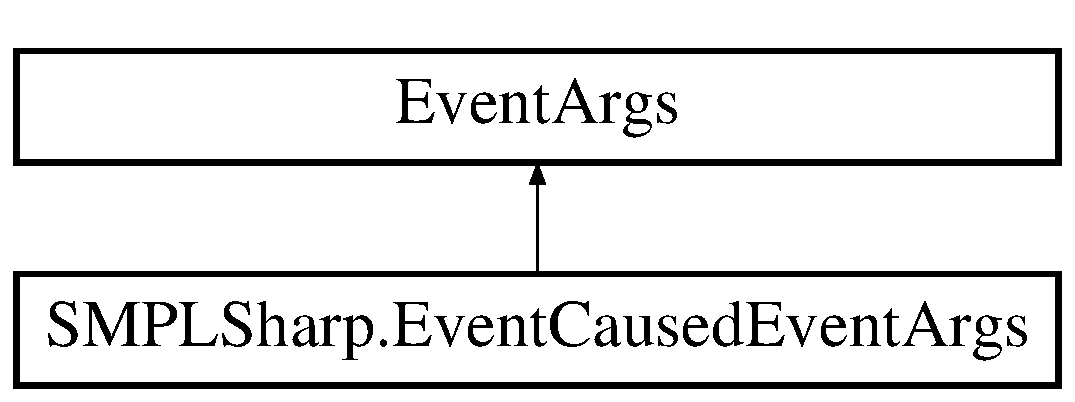
\includegraphics[height=2.000000cm]{d0/dff/class_s_m_p_l_sharp_1_1_event_caused_event_args}
\end{center}
\end{figure}
\subsection*{Открытые члены}
\begin{DoxyCompactItemize}
\item 
\hyperlink{class_s_m_p_l_sharp_1_1_event_caused_event_args_ad51196e10ac6101a36dda35b283b182e}{Event\-Caused\-Event\-Args} (\hyperlink{class_s_m_p_l_sharp_1_1_objects_1_1_smpl_event}{Smpl\-Event} model\-\_\-event)
\begin{DoxyCompactList}\small\item\em Конструктор \end{DoxyCompactList}\end{DoxyCompactItemize}
\subsection*{Свойства}
\begin{DoxyCompactItemize}
\item 
\hyperlink{class_s_m_p_l_sharp_1_1_objects_1_1_smpl_event}{Smpl\-Event} \hyperlink{class_s_m_p_l_sharp_1_1_event_caused_event_args_a80b38440396634a116a83be4a84c5c79}{Event}\hspace{0.3cm}{\ttfamily  \mbox{[}get, set\mbox{]}}
\begin{DoxyCompactList}\small\item\em Событие модели \end{DoxyCompactList}\item 
bool \hyperlink{class_s_m_p_l_sharp_1_1_event_caused_event_args_a76f44df5427c47df70a0f4eb5d1d551b}{Stop\-Model}\hspace{0.3cm}{\ttfamily  \mbox{[}get, set\mbox{]}}
\begin{DoxyCompactList}\small\item\em Если Stop\-Model == false, остановить выполнение модели (\hyperlink{class_s_m_p_l_sharp_1_1_smpl_model_a1101457a63f40e7d80e707d7793f35ee}{Smpl\-Model.\-Cause} вернет false) \end{DoxyCompactList}\end{DoxyCompactItemize}


\subsection{Подробное описание}
Event when model's event is caused 



\subsection{Конструктор(ы)}
\hypertarget{class_s_m_p_l_sharp_1_1_event_caused_event_args_ad51196e10ac6101a36dda35b283b182e}{\index{S\-M\-P\-L\-Sharp\-::\-Event\-Caused\-Event\-Args@{S\-M\-P\-L\-Sharp\-::\-Event\-Caused\-Event\-Args}!Event\-Caused\-Event\-Args@{Event\-Caused\-Event\-Args}}
\index{Event\-Caused\-Event\-Args@{Event\-Caused\-Event\-Args}!SMPLSharp::EventCausedEventArgs@{S\-M\-P\-L\-Sharp\-::\-Event\-Caused\-Event\-Args}}
\subsubsection[{Event\-Caused\-Event\-Args}]{\setlength{\rightskip}{0pt plus 5cm}S\-M\-P\-L\-Sharp.\-Event\-Caused\-Event\-Args.\-Event\-Caused\-Event\-Args (
\begin{DoxyParamCaption}
\item[{{\bf Smpl\-Event}}]{model\-\_\-event}
\end{DoxyParamCaption}
)\hspace{0.3cm}{\ttfamily [inline]}}}\label{d0/dff/class_s_m_p_l_sharp_1_1_event_caused_event_args_ad51196e10ac6101a36dda35b283b182e}


Конструктор 


\begin{DoxyParams}{Аргументы}
{\em model\-\_\-event} & Событие\\
\hline
\end{DoxyParams}


\subsection{Полный список свойств}
\hypertarget{class_s_m_p_l_sharp_1_1_event_caused_event_args_a80b38440396634a116a83be4a84c5c79}{\index{S\-M\-P\-L\-Sharp\-::\-Event\-Caused\-Event\-Args@{S\-M\-P\-L\-Sharp\-::\-Event\-Caused\-Event\-Args}!Event@{Event}}
\index{Event@{Event}!SMPLSharp::EventCausedEventArgs@{S\-M\-P\-L\-Sharp\-::\-Event\-Caused\-Event\-Args}}
\subsubsection[{Event}]{\setlength{\rightskip}{0pt plus 5cm}{\bf Smpl\-Event} S\-M\-P\-L\-Sharp.\-Event\-Caused\-Event\-Args.\-Event\hspace{0.3cm}{\ttfamily [get]}, {\ttfamily [set]}}}\label{d0/dff/class_s_m_p_l_sharp_1_1_event_caused_event_args_a80b38440396634a116a83be4a84c5c79}


Событие модели 

\hypertarget{class_s_m_p_l_sharp_1_1_event_caused_event_args_a76f44df5427c47df70a0f4eb5d1d551b}{\index{S\-M\-P\-L\-Sharp\-::\-Event\-Caused\-Event\-Args@{S\-M\-P\-L\-Sharp\-::\-Event\-Caused\-Event\-Args}!Stop\-Model@{Stop\-Model}}
\index{Stop\-Model@{Stop\-Model}!SMPLSharp::EventCausedEventArgs@{S\-M\-P\-L\-Sharp\-::\-Event\-Caused\-Event\-Args}}
\subsubsection[{Stop\-Model}]{\setlength{\rightskip}{0pt plus 5cm}bool S\-M\-P\-L\-Sharp.\-Event\-Caused\-Event\-Args.\-Stop\-Model\hspace{0.3cm}{\ttfamily [get]}, {\ttfamily [set]}}}\label{d0/dff/class_s_m_p_l_sharp_1_1_event_caused_event_args_a76f44df5427c47df70a0f4eb5d1d551b}


Если Stop\-Model == false, остановить выполнение модели (\hyperlink{class_s_m_p_l_sharp_1_1_smpl_model_a1101457a63f40e7d80e707d7793f35ee}{Smpl\-Model.\-Cause} вернет false) 



Объявления и описания членов класса находятся в файле\-:\begin{DoxyCompactItemize}
\item 
D\-:/\-My Documents/\-Git\-Hub/\-S\-M\-P\-L\-Sharp/\-S\-M\-P\-L\-Sharp/Smpl\-Model.\-cs\end{DoxyCompactItemize}

\hypertarget{class_s_m_p_l_sharp_1_1_objects_1_1_smpl_device}{\section{Класс S\-M\-P\-L\-Sharp.\-Objects.\-Smpl\-Device}
\label{d7/d39/class_s_m_p_l_sharp_1_1_objects_1_1_smpl_device}\index{S\-M\-P\-L\-Sharp.\-Objects.\-Smpl\-Device@{S\-M\-P\-L\-Sharp.\-Objects.\-Smpl\-Device}}
}


Equipment or facility Typically represents some work-\/performing resource of system being modeled The Interconnection of facilities is not explicit, but can be determined by the model’s routing of tokens between facilities  


\subsection*{Открытые члены}
\begin{DoxyCompactItemize}
\item 
void \hyperlink{class_s_m_p_l_sharp_1_1_objects_1_1_smpl_device_a43be17c0606bf8f720149c2777a33e31}{Reserve} ()
\begin{DoxyCompactList}\small\item\em Зарезервировать прибор (param = 1) \end{DoxyCompactList}\item 
void \hyperlink{class_s_m_p_l_sharp_1_1_objects_1_1_smpl_device_a8fac05272f1a7e1213336639e3453512}{Reserve} (object token)
\begin{DoxyCompactList}\small\item\em Зарезервировать прибор и поменять его статус на param. В случае передачи token == null, прибор будет освобожден. Если прибор занаят, то происходит исключение с текстом ошибки. \end{DoxyCompactList}\item 
void \hyperlink{class_s_m_p_l_sharp_1_1_objects_1_1_smpl_device_a81feb298bcfe5e7c87cd0e91a1a329ce}{Release} ()
\begin{DoxyCompactList}\small\item\em Освободить прибор \end{DoxyCompactList}\end{DoxyCompactItemize}
\subsection*{Свойства}
\begin{DoxyCompactItemize}
\item 
virtual string \hyperlink{class_s_m_p_l_sharp_1_1_objects_1_1_smpl_device_a3525605581b83649d988ca1326b4732f}{Name}\hspace{0.3cm}{\ttfamily  \mbox{[}get, set\mbox{]}}
\begin{DoxyCompactList}\small\item\em Имя прибора \end{DoxyCompactList}\item 
virtual object \hyperlink{class_s_m_p_l_sharp_1_1_objects_1_1_smpl_device_a2e79fee0f480adec487fdf013ed52b2a}{Status}\hspace{0.3cm}{\ttfamily  \mbox{[}get, set\mbox{]}}
\begin{DoxyCompactList}\small\item\em Состояние прибора. Если Status == null, прибор свободен \end{DoxyCompactList}\item 
bool \hyperlink{class_s_m_p_l_sharp_1_1_objects_1_1_smpl_device_a7e6939193f240d5f5642e07ef7d6b73e}{Is\-Busy}\hspace{0.3cm}{\ttfamily  \mbox{[}get\mbox{]}}
\begin{DoxyCompactList}\small\item\em Прибор занят? \end{DoxyCompactList}\item 
virtual int \hyperlink{class_s_m_p_l_sharp_1_1_objects_1_1_smpl_device_a8757abb401c1dfa7093ced84f715a2d2}{Time\-Last\-Reserved}\hspace{0.3cm}{\ttfamily  \mbox{[}get, set\mbox{]}}
\begin{DoxyCompactList}\small\item\em Время последнего вызова Reserve \end{DoxyCompactList}\item 
virtual int \hyperlink{class_s_m_p_l_sharp_1_1_objects_1_1_smpl_device_afe478b9c4ec74e462f5af5d3a51f4131}{Time\-Total\-Reserved}\hspace{0.3cm}{\ttfamily  \mbox{[}get, set\mbox{]}}
\begin{DoxyCompactList}\small\item\em Суммарное время, пока прибор занят \end{DoxyCompactList}\item 
virtual int \hyperlink{class_s_m_p_l_sharp_1_1_objects_1_1_smpl_device_a675ca052cc3996e38aec7ccc1dd7ca8c}{Query\-Counter}\hspace{0.3cm}{\ttfamily  \mbox{[}get, set\mbox{]}}
\begin{DoxyCompactList}\small\item\em Счетчик запросов (пар вызовов reserve/release) \end{DoxyCompactList}\item 
\hyperlink{class_s_m_p_l_sharp_1_1_smpl_model}{Smpl\-Model} \hyperlink{class_s_m_p_l_sharp_1_1_objects_1_1_smpl_device_ad4036c2596ab7029b778ad45090df69b}{Model}\hspace{0.3cm}{\ttfamily  \mbox{[}get, set\mbox{]}}
\begin{DoxyCompactList}\small\item\em Модель, с которой связан прибор \end{DoxyCompactList}\end{DoxyCompactItemize}


\subsection{Подробное описание}
Equipment or facility Typically represents some work-\/performing resource of system being modeled The Interconnection of facilities is not explicit, but can be determined by the model’s routing of tokens between facilities 



См. определение в файле Smpl\-Device.\-cs строка 21



\subsection{Методы}
\hypertarget{class_s_m_p_l_sharp_1_1_objects_1_1_smpl_device_a81feb298bcfe5e7c87cd0e91a1a329ce}{\index{S\-M\-P\-L\-Sharp\-::\-Objects\-::\-Smpl\-Device@{S\-M\-P\-L\-Sharp\-::\-Objects\-::\-Smpl\-Device}!Release@{Release}}
\index{Release@{Release}!SMPLSharp::Objects::SmplDevice@{S\-M\-P\-L\-Sharp\-::\-Objects\-::\-Smpl\-Device}}
\subsubsection[{Release}]{\setlength{\rightskip}{0pt plus 5cm}void S\-M\-P\-L\-Sharp.\-Objects.\-Smpl\-Device.\-Release (
\begin{DoxyParamCaption}
{}
\end{DoxyParamCaption}
)}}\label{d7/d39/class_s_m_p_l_sharp_1_1_objects_1_1_smpl_device_a81feb298bcfe5e7c87cd0e91a1a329ce}


Освободить прибор 



См. определение в файле Smpl\-Device.\-cs строка 149

\hypertarget{class_s_m_p_l_sharp_1_1_objects_1_1_smpl_device_a43be17c0606bf8f720149c2777a33e31}{\index{S\-M\-P\-L\-Sharp\-::\-Objects\-::\-Smpl\-Device@{S\-M\-P\-L\-Sharp\-::\-Objects\-::\-Smpl\-Device}!Reserve@{Reserve}}
\index{Reserve@{Reserve}!SMPLSharp::Objects::SmplDevice@{S\-M\-P\-L\-Sharp\-::\-Objects\-::\-Smpl\-Device}}
\subsubsection[{Reserve}]{\setlength{\rightskip}{0pt plus 5cm}void S\-M\-P\-L\-Sharp.\-Objects.\-Smpl\-Device.\-Reserve (
\begin{DoxyParamCaption}
{}
\end{DoxyParamCaption}
)}}\label{d7/d39/class_s_m_p_l_sharp_1_1_objects_1_1_smpl_device_a43be17c0606bf8f720149c2777a33e31}


Зарезервировать прибор (param = 1) 



См. определение в файле Smpl\-Device.\-cs строка 115

\hypertarget{class_s_m_p_l_sharp_1_1_objects_1_1_smpl_device_a8fac05272f1a7e1213336639e3453512}{\index{S\-M\-P\-L\-Sharp\-::\-Objects\-::\-Smpl\-Device@{S\-M\-P\-L\-Sharp\-::\-Objects\-::\-Smpl\-Device}!Reserve@{Reserve}}
\index{Reserve@{Reserve}!SMPLSharp::Objects::SmplDevice@{S\-M\-P\-L\-Sharp\-::\-Objects\-::\-Smpl\-Device}}
\subsubsection[{Reserve}]{\setlength{\rightskip}{0pt plus 5cm}void S\-M\-P\-L\-Sharp.\-Objects.\-Smpl\-Device.\-Reserve (
\begin{DoxyParamCaption}
\item[{object}]{token}
\end{DoxyParamCaption}
)}}\label{d7/d39/class_s_m_p_l_sharp_1_1_objects_1_1_smpl_device_a8fac05272f1a7e1213336639e3453512}


Зарезервировать прибор и поменять его статус на param. В случае передачи token == null, прибор будет освобожден. Если прибор занаят, то происходит исключение с текстом ошибки. 


\begin{DoxyParams}{Аргументы}
{\em token} & параметр\\
\hline
\end{DoxyParams}


См. определение в файле Smpl\-Device.\-cs строка 124



\subsection{Полный список свойств}
\hypertarget{class_s_m_p_l_sharp_1_1_objects_1_1_smpl_device_a7e6939193f240d5f5642e07ef7d6b73e}{\index{S\-M\-P\-L\-Sharp\-::\-Objects\-::\-Smpl\-Device@{S\-M\-P\-L\-Sharp\-::\-Objects\-::\-Smpl\-Device}!Is\-Busy@{Is\-Busy}}
\index{Is\-Busy@{Is\-Busy}!SMPLSharp::Objects::SmplDevice@{S\-M\-P\-L\-Sharp\-::\-Objects\-::\-Smpl\-Device}}
\subsubsection[{Is\-Busy}]{\setlength{\rightskip}{0pt plus 5cm}bool S\-M\-P\-L\-Sharp.\-Objects.\-Smpl\-Device.\-Is\-Busy\hspace{0.3cm}{\ttfamily [get]}}}\label{d7/d39/class_s_m_p_l_sharp_1_1_objects_1_1_smpl_device_a7e6939193f240d5f5642e07ef7d6b73e}


Прибор занят? 



См. определение в файле Smpl\-Device.\-cs строка 48

\hypertarget{class_s_m_p_l_sharp_1_1_objects_1_1_smpl_device_ad4036c2596ab7029b778ad45090df69b}{\index{S\-M\-P\-L\-Sharp\-::\-Objects\-::\-Smpl\-Device@{S\-M\-P\-L\-Sharp\-::\-Objects\-::\-Smpl\-Device}!Model@{Model}}
\index{Model@{Model}!SMPLSharp::Objects::SmplDevice@{S\-M\-P\-L\-Sharp\-::\-Objects\-::\-Smpl\-Device}}
\subsubsection[{Model}]{\setlength{\rightskip}{0pt plus 5cm}{\bf Smpl\-Model} S\-M\-P\-L\-Sharp.\-Objects.\-Smpl\-Device.\-Model\hspace{0.3cm}{\ttfamily [get]}, {\ttfamily [set]}}}\label{d7/d39/class_s_m_p_l_sharp_1_1_objects_1_1_smpl_device_ad4036c2596ab7029b778ad45090df69b}


Модель, с которой связан прибор 



См. определение в файле Smpl\-Device.\-cs строка 83

\hypertarget{class_s_m_p_l_sharp_1_1_objects_1_1_smpl_device_a3525605581b83649d988ca1326b4732f}{\index{S\-M\-P\-L\-Sharp\-::\-Objects\-::\-Smpl\-Device@{S\-M\-P\-L\-Sharp\-::\-Objects\-::\-Smpl\-Device}!Name@{Name}}
\index{Name@{Name}!SMPLSharp::Objects::SmplDevice@{S\-M\-P\-L\-Sharp\-::\-Objects\-::\-Smpl\-Device}}
\subsubsection[{Name}]{\setlength{\rightskip}{0pt plus 5cm}virtual string S\-M\-P\-L\-Sharp.\-Objects.\-Smpl\-Device.\-Name\hspace{0.3cm}{\ttfamily [get]}, {\ttfamily [set]}}}\label{d7/d39/class_s_m_p_l_sharp_1_1_objects_1_1_smpl_device_a3525605581b83649d988ca1326b4732f}


Имя прибора 



См. определение в файле Smpl\-Device.\-cs строка 30

\hypertarget{class_s_m_p_l_sharp_1_1_objects_1_1_smpl_device_a675ca052cc3996e38aec7ccc1dd7ca8c}{\index{S\-M\-P\-L\-Sharp\-::\-Objects\-::\-Smpl\-Device@{S\-M\-P\-L\-Sharp\-::\-Objects\-::\-Smpl\-Device}!Query\-Counter@{Query\-Counter}}
\index{Query\-Counter@{Query\-Counter}!SMPLSharp::Objects::SmplDevice@{S\-M\-P\-L\-Sharp\-::\-Objects\-::\-Smpl\-Device}}
\subsubsection[{Query\-Counter}]{\setlength{\rightskip}{0pt plus 5cm}virtual int S\-M\-P\-L\-Sharp.\-Objects.\-Smpl\-Device.\-Query\-Counter\hspace{0.3cm}{\ttfamily [get]}, {\ttfamily [set]}}}\label{d7/d39/class_s_m_p_l_sharp_1_1_objects_1_1_smpl_device_a675ca052cc3996e38aec7ccc1dd7ca8c}


Счетчик запросов (пар вызовов reserve/release) 



См. определение в файле Smpl\-Device.\-cs строка 74

\hypertarget{class_s_m_p_l_sharp_1_1_objects_1_1_smpl_device_a2e79fee0f480adec487fdf013ed52b2a}{\index{S\-M\-P\-L\-Sharp\-::\-Objects\-::\-Smpl\-Device@{S\-M\-P\-L\-Sharp\-::\-Objects\-::\-Smpl\-Device}!Status@{Status}}
\index{Status@{Status}!SMPLSharp::Objects::SmplDevice@{S\-M\-P\-L\-Sharp\-::\-Objects\-::\-Smpl\-Device}}
\subsubsection[{Status}]{\setlength{\rightskip}{0pt plus 5cm}virtual object S\-M\-P\-L\-Sharp.\-Objects.\-Smpl\-Device.\-Status\hspace{0.3cm}{\ttfamily [get]}, {\ttfamily [set]}}}\label{d7/d39/class_s_m_p_l_sharp_1_1_objects_1_1_smpl_device_a2e79fee0f480adec487fdf013ed52b2a}


Состояние прибора. Если Status == null, прибор свободен 



См. определение в файле Smpl\-Device.\-cs строка 39

\hypertarget{class_s_m_p_l_sharp_1_1_objects_1_1_smpl_device_a8757abb401c1dfa7093ced84f715a2d2}{\index{S\-M\-P\-L\-Sharp\-::\-Objects\-::\-Smpl\-Device@{S\-M\-P\-L\-Sharp\-::\-Objects\-::\-Smpl\-Device}!Time\-Last\-Reserved@{Time\-Last\-Reserved}}
\index{Time\-Last\-Reserved@{Time\-Last\-Reserved}!SMPLSharp::Objects::SmplDevice@{S\-M\-P\-L\-Sharp\-::\-Objects\-::\-Smpl\-Device}}
\subsubsection[{Time\-Last\-Reserved}]{\setlength{\rightskip}{0pt plus 5cm}virtual int S\-M\-P\-L\-Sharp.\-Objects.\-Smpl\-Device.\-Time\-Last\-Reserved\hspace{0.3cm}{\ttfamily [get]}, {\ttfamily [set]}}}\label{d7/d39/class_s_m_p_l_sharp_1_1_objects_1_1_smpl_device_a8757abb401c1dfa7093ced84f715a2d2}


Время последнего вызова Reserve 



См. определение в файле Smpl\-Device.\-cs строка 56

\hypertarget{class_s_m_p_l_sharp_1_1_objects_1_1_smpl_device_afe478b9c4ec74e462f5af5d3a51f4131}{\index{S\-M\-P\-L\-Sharp\-::\-Objects\-::\-Smpl\-Device@{S\-M\-P\-L\-Sharp\-::\-Objects\-::\-Smpl\-Device}!Time\-Total\-Reserved@{Time\-Total\-Reserved}}
\index{Time\-Total\-Reserved@{Time\-Total\-Reserved}!SMPLSharp::Objects::SmplDevice@{S\-M\-P\-L\-Sharp\-::\-Objects\-::\-Smpl\-Device}}
\subsubsection[{Time\-Total\-Reserved}]{\setlength{\rightskip}{0pt plus 5cm}virtual int S\-M\-P\-L\-Sharp.\-Objects.\-Smpl\-Device.\-Time\-Total\-Reserved\hspace{0.3cm}{\ttfamily [get]}, {\ttfamily [set]}}}\label{d7/d39/class_s_m_p_l_sharp_1_1_objects_1_1_smpl_device_afe478b9c4ec74e462f5af5d3a51f4131}


Суммарное время, пока прибор занят 



См. определение в файле Smpl\-Device.\-cs строка 65



Объявления и описания членов класса находятся в файле\-:\begin{DoxyCompactItemize}
\item 
D\-:/\-My Documents/\-Git\-Hub/\-S\-M\-P\-L\-Sharp/\-S\-M\-P\-L\-Sharp/Smpl\-Device.\-cs\end{DoxyCompactItemize}

\hypertarget{class_s_m_p_l_sharp_1_1_objects_1_1_smpl_event}{\section{Класс S\-M\-P\-L\-Sharp.\-Objects.\-Smpl\-Event}
\label{de/d57/class_s_m_p_l_sharp_1_1_objects_1_1_smpl_event}\index{S\-M\-P\-L\-Sharp.\-Objects.\-Smpl\-Event@{S\-M\-P\-L\-Sharp.\-Objects.\-Smpl\-Event}}
}


Model's event A change of state of any system entity, active or passive Can be, for example, Arrival of task or Computing completion  


\subsection*{Свойства}
\begin{DoxyCompactItemize}
\item 
virtual int \hyperlink{class_s_m_p_l_sharp_1_1_objects_1_1_smpl_event_a7ee1edd67c31aef8cd818f899a393abe}{Event\-I\-D}\hspace{0.3cm}{\ttfamily  \mbox{[}get, set\mbox{]}}
\begin{DoxyCompactList}\small\item\em Идентификатор типа события \end{DoxyCompactList}\item 
virtual int \hyperlink{class_s_m_p_l_sharp_1_1_objects_1_1_smpl_event_a5d72178bd46b26372514d711c05a3ea2}{Time\-Registred}\hspace{0.3cm}{\ttfamily  \mbox{[}get, set\mbox{]}}
\begin{DoxyCompactList}\small\item\em Время регистрации в модели \end{DoxyCompactList}\item 
virtual int \hyperlink{class_s_m_p_l_sharp_1_1_objects_1_1_smpl_event_ad5ad0f4179e5d77831cc82d0a8bf5b29}{Time\-Caused}\hspace{0.3cm}{\ttfamily  \mbox{[}get, set\mbox{]}}
\begin{DoxyCompactList}\small\item\em Время возникновения в модели (Time\-Registred + время ожидания) \end{DoxyCompactList}\item 
virtual object \hyperlink{class_s_m_p_l_sharp_1_1_objects_1_1_smpl_event_ae4cc80e480603021bc0d0d0e1ea2c666}{Param}\hspace{0.3cm}{\ttfamily  \mbox{[}get, set\mbox{]}}
\begin{DoxyCompactList}\small\item\em Доп. параметр события \end{DoxyCompactList}\end{DoxyCompactItemize}


\subsection{Подробное описание}
Model's event A change of state of any system entity, active or passive Can be, for example, Arrival of task or Computing completion 



\subsection{Полный список свойств}
\hypertarget{class_s_m_p_l_sharp_1_1_objects_1_1_smpl_event_a7ee1edd67c31aef8cd818f899a393abe}{\index{S\-M\-P\-L\-Sharp\-::\-Objects\-::\-Smpl\-Event@{S\-M\-P\-L\-Sharp\-::\-Objects\-::\-Smpl\-Event}!Event\-I\-D@{Event\-I\-D}}
\index{Event\-I\-D@{Event\-I\-D}!SMPLSharp::Objects::SmplEvent@{S\-M\-P\-L\-Sharp\-::\-Objects\-::\-Smpl\-Event}}
\subsubsection[{Event\-I\-D}]{\setlength{\rightskip}{0pt plus 5cm}virtual int S\-M\-P\-L\-Sharp.\-Objects.\-Smpl\-Event.\-Event\-I\-D\hspace{0.3cm}{\ttfamily [get]}, {\ttfamily [set]}}}\label{de/d57/class_s_m_p_l_sharp_1_1_objects_1_1_smpl_event_a7ee1edd67c31aef8cd818f899a393abe}


Идентификатор типа события 

\hypertarget{class_s_m_p_l_sharp_1_1_objects_1_1_smpl_event_ae4cc80e480603021bc0d0d0e1ea2c666}{\index{S\-M\-P\-L\-Sharp\-::\-Objects\-::\-Smpl\-Event@{S\-M\-P\-L\-Sharp\-::\-Objects\-::\-Smpl\-Event}!Param@{Param}}
\index{Param@{Param}!SMPLSharp::Objects::SmplEvent@{S\-M\-P\-L\-Sharp\-::\-Objects\-::\-Smpl\-Event}}
\subsubsection[{Param}]{\setlength{\rightskip}{0pt plus 5cm}virtual object S\-M\-P\-L\-Sharp.\-Objects.\-Smpl\-Event.\-Param\hspace{0.3cm}{\ttfamily [get]}, {\ttfamily [set]}}}\label{de/d57/class_s_m_p_l_sharp_1_1_objects_1_1_smpl_event_ae4cc80e480603021bc0d0d0e1ea2c666}


Доп. параметр события 

\hypertarget{class_s_m_p_l_sharp_1_1_objects_1_1_smpl_event_ad5ad0f4179e5d77831cc82d0a8bf5b29}{\index{S\-M\-P\-L\-Sharp\-::\-Objects\-::\-Smpl\-Event@{S\-M\-P\-L\-Sharp\-::\-Objects\-::\-Smpl\-Event}!Time\-Caused@{Time\-Caused}}
\index{Time\-Caused@{Time\-Caused}!SMPLSharp::Objects::SmplEvent@{S\-M\-P\-L\-Sharp\-::\-Objects\-::\-Smpl\-Event}}
\subsubsection[{Time\-Caused}]{\setlength{\rightskip}{0pt plus 5cm}virtual int S\-M\-P\-L\-Sharp.\-Objects.\-Smpl\-Event.\-Time\-Caused\hspace{0.3cm}{\ttfamily [get]}, {\ttfamily [set]}}}\label{de/d57/class_s_m_p_l_sharp_1_1_objects_1_1_smpl_event_ad5ad0f4179e5d77831cc82d0a8bf5b29}


Время возникновения в модели (Time\-Registred + время ожидания) 

\hypertarget{class_s_m_p_l_sharp_1_1_objects_1_1_smpl_event_a5d72178bd46b26372514d711c05a3ea2}{\index{S\-M\-P\-L\-Sharp\-::\-Objects\-::\-Smpl\-Event@{S\-M\-P\-L\-Sharp\-::\-Objects\-::\-Smpl\-Event}!Time\-Registred@{Time\-Registred}}
\index{Time\-Registred@{Time\-Registred}!SMPLSharp::Objects::SmplEvent@{S\-M\-P\-L\-Sharp\-::\-Objects\-::\-Smpl\-Event}}
\subsubsection[{Time\-Registred}]{\setlength{\rightskip}{0pt plus 5cm}virtual int S\-M\-P\-L\-Sharp.\-Objects.\-Smpl\-Event.\-Time\-Registred\hspace{0.3cm}{\ttfamily [get]}, {\ttfamily [set]}}}\label{de/d57/class_s_m_p_l_sharp_1_1_objects_1_1_smpl_event_a5d72178bd46b26372514d711c05a3ea2}


Время регистрации в модели 



Объявления и описания членов класса находятся в файле\-:\begin{DoxyCompactItemize}
\item 
D\-:/\-My Documents/\-Git\-Hub/\-S\-M\-P\-L\-Sharp/\-S\-M\-P\-L\-Sharp/Smpl\-Event.\-cs\end{DoxyCompactItemize}

\hypertarget{class_s_m_p_l_sharp_1_1_smpl_model}{\section{Класс S\-M\-P\-L\-Sharp.\-Smpl\-Model}
\label{df/d34/class_s_m_p_l_sharp_1_1_smpl_model}\index{S\-M\-P\-L\-Sharp.\-Smpl\-Model@{S\-M\-P\-L\-Sharp.\-Smpl\-Model}}
}


Simulation model. Provides set of function for building event-\/based, discrete-\/event simulation model  


\subsection*{Открытые члены}
\begin{DoxyCompactItemize}
\item 
\hyperlink{class_s_m_p_l_sharp_1_1_smpl_model_af44997fa13bc821115726c45c7aaad7a}{Smpl\-Model} ()
\begin{DoxyCompactList}\small\item\em Конструктор \end{DoxyCompactList}\item 
virtual \hyperlink{class_s_m_p_l_sharp_1_1_objects_1_1_smpl_queue}{Smpl\-Queue} \hyperlink{class_s_m_p_l_sharp_1_1_smpl_model_ac95017a5bdb0500bb655791303d7cbb2}{Create\-Queue} (string name)
\begin{DoxyCompactList}\small\item\em Добавить очередь в модель \end{DoxyCompactList}\item 
virtual \hyperlink{class_s_m_p_l_sharp_1_1_objects_1_1_smpl_queue}{Smpl\-Queue} \hyperlink{class_s_m_p_l_sharp_1_1_smpl_model_a8c61642d973fd1da0996a3ab0e04b3cc}{Queue} (string name)
\begin{DoxyCompactList}\small\item\em Возвратить существующую очередь \end{DoxyCompactList}\item 
virtual \hyperlink{class_s_m_p_l_sharp_1_1_objects_1_1_smpl_device}{Smpl\-Device} \hyperlink{class_s_m_p_l_sharp_1_1_smpl_model_a1a36f287db98f6e73760dc8f7c2d0497}{Create\-Device} (string name)
\begin{DoxyCompactList}\small\item\em Добавить прибор в модель \end{DoxyCompactList}\item 
virtual \hyperlink{class_s_m_p_l_sharp_1_1_objects_1_1_smpl_device}{Smpl\-Device} \hyperlink{class_s_m_p_l_sharp_1_1_smpl_model_a0c48f93d0d086ef9e340f29a3664fb55}{Device} (string name)
\begin{DoxyCompactList}\small\item\em Возвратить существующий прибор \end{DoxyCompactList}\item 
virtual \hyperlink{class_s_m_p_l_sharp_1_1_objects_1_1_smpl_multi_device}{Smpl\-Multi\-Device} \hyperlink{class_s_m_p_l_sharp_1_1_smpl_model_a661c9fcf2482f3961c594b4a8d8b5f96}{Create\-Multi\-Device} (string name, int count\-Ambary)
\begin{DoxyCompactList}\small\item\em Добавить многоканальный прибор в модель \end{DoxyCompactList}\item 
virtual \hyperlink{class_s_m_p_l_sharp_1_1_objects_1_1_smpl_multi_device}{Smpl\-Multi\-Device} \hyperlink{class_s_m_p_l_sharp_1_1_smpl_model_a42d73f3d756bbf0375ba2012c708441d}{Multi\-Device} (string name)
\begin{DoxyCompactList}\small\item\em Возвратить существующий многоканальный прибор \end{DoxyCompactList}\item 
void \hyperlink{class_s_m_p_l_sharp_1_1_smpl_model_af567f319b044a2c6c98a80bff589ad04}{Schedule} (int event\-\_\-id, int wait\-\_\-time, object param=null)
\begin{DoxyCompactList}\small\item\em Запланировать событие \end{DoxyCompactList}\item 
bool \hyperlink{class_s_m_p_l_sharp_1_1_smpl_model_a1101457a63f40e7d80e707d7793f35ee}{Cause} (out \hyperlink{class_s_m_p_l_sharp_1_1_objects_1_1_smpl_event}{Smpl\-Event} model\-\_\-event)
\begin{DoxyCompactList}\small\item\em Вызвать ближайшее событие модели \end{DoxyCompactList}\item 
bool \hyperlink{class_s_m_p_l_sharp_1_1_smpl_model_ae2da4d875550fe62753443c0a7a276ee}{Cause} ()
\begin{DoxyCompactList}\small\item\em Вызвать ближайшее событие модели \end{DoxyCompactList}\item 
bool \hyperlink{class_s_m_p_l_sharp_1_1_smpl_model_a033dfe1b24a1864b7a4c8a85831aafd3}{Cause} (out int event\-\_\-id, out object param)
\begin{DoxyCompactList}\small\item\em Вызвать ближайшее событие модели \end{DoxyCompactList}\item 
int \hyperlink{class_s_m_p_l_sharp_1_1_smpl_model_a2af716a4608f04a0ec2814d921c5197e}{Cancel} (int event\-\_\-id, object param=null)
\begin{DoxyCompactList}\small\item\em Отменить ближайшее запланированное событие с указанными параметрами \end{DoxyCompactList}\item 
int \hyperlink{class_s_m_p_l_sharp_1_1_smpl_model_a77390fc51749077e44b0285a76faf5cc}{I\-Random} (int a, int b)
\begin{DoxyCompactList}\small\item\em Генерирует число по равномерному распределению в диапозоне \mbox{[}a, b\mbox{]} включительно \end{DoxyCompactList}\item 
int \hyperlink{class_s_m_p_l_sharp_1_1_smpl_model_aa89b976daa026bf83a1a2818d34abfa0}{I\-Random} (int a)
\begin{DoxyCompactList}\small\item\em Генерирует число по равномерному распределению в диапозоне \mbox{[}0, a\mbox{]} включительно \end{DoxyCompactList}\item 
int \hyperlink{class_s_m_p_l_sharp_1_1_smpl_model_a2a899ce5ab2a8a7b127a962c33b047e4}{Nex\-Exp} (int m)
\begin{DoxyCompactList}\small\item\em Генерирует число по отрицательному экспоненциальному распределению со средней точкой m \end{DoxyCompactList}\item 
string \hyperlink{class_s_m_p_l_sharp_1_1_smpl_model_a221aa0af22ddc3dcc9860df9a76eb96e}{Report} ()
\begin{DoxyCompactList}\small\item\em Генерирует стандартный отчет о модели \end{DoxyCompactList}\end{DoxyCompactItemize}
\subsection*{Защищенные члены}
\begin{DoxyCompactItemize}
\item 
virtual bool \hyperlink{class_s_m_p_l_sharp_1_1_smpl_model_a855ce8850f451bb372a12c9a02c2b422}{On\-Event\-Caused} (\hyperlink{class_s_m_p_l_sharp_1_1_event_caused_event_args}{Event\-Caused\-Event\-Args} e)
\begin{DoxyCompactList}\small\item\em Событие возникновения события модели. Возникает при вызове Cause \end{DoxyCompactList}\end{DoxyCompactItemize}
\subsection*{Защищенные данные}
\begin{DoxyCompactItemize}
\item 
Dictionary$<$ string, \hyperlink{class_s_m_p_l_sharp_1_1_objects_1_1_smpl_queue}{Smpl\-Queue} $>$ \hyperlink{class_s_m_p_l_sharp_1_1_smpl_model_ace458c3e9bb07de68137027426eeee82}{queues}
\begin{DoxyCompactList}\small\item\em Очереди модели \end{DoxyCompactList}\item 
Dictionary$<$ string, \hyperlink{class_s_m_p_l_sharp_1_1_objects_1_1_smpl_device}{Smpl\-Device} $>$ \hyperlink{class_s_m_p_l_sharp_1_1_smpl_model_a1dcd953a3d955e2fde2edc4101a7d0cf}{devices}
\begin{DoxyCompactList}\small\item\em Приборы модели \end{DoxyCompactList}\item 
List$<$ \hyperlink{class_s_m_p_l_sharp_1_1_objects_1_1_smpl_event}{Smpl\-Event} $>$ \hyperlink{class_s_m_p_l_sharp_1_1_smpl_model_ac57b9b5e15eb34682873492bab42445f}{future\-Events}
\begin{DoxyCompactList}\small\item\em Журнал будущих событий модели \end{DoxyCompactList}\item 
Dictionary$<$ string, \\*
\hyperlink{class_s_m_p_l_sharp_1_1_objects_1_1_smpl_multi_device}{Smpl\-Multi\-Device} $>$ \hyperlink{class_s_m_p_l_sharp_1_1_smpl_model_a711b2226de9b75bd541ddca587fb5e45}{multi\-Devices}
\begin{DoxyCompactList}\small\item\em Многоканальные приборы модели \end{DoxyCompactList}\end{DoxyCompactItemize}
\subsection*{Свойства}
\begin{DoxyCompactItemize}
\item 
virtual \hyperlink{class_s_m_p_l_sharp_1_1_utils_1_1_smpl_random_generator}{Smpl\-Random\-Generator} \hyperlink{class_s_m_p_l_sharp_1_1_smpl_model_a0f7a947d68471f69ba6afaf03ec15093}{Rand\-Gen}\hspace{0.3cm}{\ttfamily  \mbox{[}get, set\mbox{]}}
\begin{DoxyCompactList}\small\item\em Генератор случайных чисел \end{DoxyCompactList}\item 
virtual int \hyperlink{class_s_m_p_l_sharp_1_1_smpl_model_a091e0759cad46e82a02ff253a232a37d}{Time}\hspace{0.3cm}{\ttfamily  \mbox{[}get, set\mbox{]}}
\begin{DoxyCompactList}\small\item\em Модельное время \end{DoxyCompactList}\item 
virtual int \hyperlink{class_s_m_p_l_sharp_1_1_smpl_model_a83863cdbfb43901325e891a65fd27d40}{Next\-Event\-Time}\hspace{0.3cm}{\ttfamily  \mbox{[}get\mbox{]}}
\begin{DoxyCompactList}\small\item\em Время следующего события \end{DoxyCompactList}\item 
virtual bool \hyperlink{class_s_m_p_l_sharp_1_1_smpl_model_a5427e31d8b72ff5823518e5eff801fd3}{Is\-Stopped}\hspace{0.3cm}{\ttfamily  \mbox{[}get, set\mbox{]}}
\begin{DoxyCompactList}\small\item\em Модель была остановлена \end{DoxyCompactList}\item 
virtual Dictionary$<$ string, \\*
\hyperlink{class_s_m_p_l_sharp_1_1_objects_1_1_smpl_queue}{Smpl\-Queue} $>$ \hyperlink{class_s_m_p_l_sharp_1_1_smpl_model_a1bbb9a6e7a49ca06902fa90aa611c719}{Queues}\hspace{0.3cm}{\ttfamily  \mbox{[}get\mbox{]}}
\begin{DoxyCompactList}\small\item\em Очереди \end{DoxyCompactList}\item 
virtual Dictionary$<$ string, \\*
\hyperlink{class_s_m_p_l_sharp_1_1_objects_1_1_smpl_device}{Smpl\-Device} $>$ \hyperlink{class_s_m_p_l_sharp_1_1_smpl_model_af79bc37f93c34d07abbdf36028581640}{Devices}\hspace{0.3cm}{\ttfamily  \mbox{[}get\mbox{]}}
\begin{DoxyCompactList}\small\item\em Приборы \end{DoxyCompactList}\item 
virtual Dictionary$<$ string, \\*
\hyperlink{class_s_m_p_l_sharp_1_1_objects_1_1_smpl_multi_device}{Smpl\-Multi\-Device} $>$ \hyperlink{class_s_m_p_l_sharp_1_1_smpl_model_a6a37ccf8af439fc11b156eff04514e2e}{Multi\-Devices}\hspace{0.3cm}{\ttfamily  \mbox{[}get\mbox{]}}
\begin{DoxyCompactList}\small\item\em Многоканальные приборы \end{DoxyCompactList}\end{DoxyCompactItemize}
\subsection*{События}
\begin{DoxyCompactItemize}
\item 
\hyperlink{namespace_s_m_p_l_sharp_a33fb2904b12541599362cddd40c71357}{Event\-Caused\-Handler} \hyperlink{class_s_m_p_l_sharp_1_1_smpl_model_abfa9344a73f4845e02be97fd5b963ed3}{Event\-Caused}
\begin{DoxyCompactList}\small\item\em Событие соершено \end{DoxyCompactList}\end{DoxyCompactItemize}


\subsection{Подробное описание}
Simulation model. Provides set of function for building event-\/based, discrete-\/event simulation model 



\subsection{Конструктор(ы)}
\hypertarget{class_s_m_p_l_sharp_1_1_smpl_model_af44997fa13bc821115726c45c7aaad7a}{\index{S\-M\-P\-L\-Sharp\-::\-Smpl\-Model@{S\-M\-P\-L\-Sharp\-::\-Smpl\-Model}!Smpl\-Model@{Smpl\-Model}}
\index{Smpl\-Model@{Smpl\-Model}!SMPLSharp::SmplModel@{S\-M\-P\-L\-Sharp\-::\-Smpl\-Model}}
\subsubsection[{Smpl\-Model}]{\setlength{\rightskip}{0pt plus 5cm}S\-M\-P\-L\-Sharp.\-Smpl\-Model.\-Smpl\-Model (
\begin{DoxyParamCaption}
{}
\end{DoxyParamCaption}
)\hspace{0.3cm}{\ttfamily [inline]}}}\label{df/d34/class_s_m_p_l_sharp_1_1_smpl_model_af44997fa13bc821115726c45c7aaad7a}


Конструктор 



\subsection{Методы}
\hypertarget{class_s_m_p_l_sharp_1_1_smpl_model_a2af716a4608f04a0ec2814d921c5197e}{\index{S\-M\-P\-L\-Sharp\-::\-Smpl\-Model@{S\-M\-P\-L\-Sharp\-::\-Smpl\-Model}!Cancel@{Cancel}}
\index{Cancel@{Cancel}!SMPLSharp::SmplModel@{S\-M\-P\-L\-Sharp\-::\-Smpl\-Model}}
\subsubsection[{Cancel}]{\setlength{\rightskip}{0pt plus 5cm}int S\-M\-P\-L\-Sharp.\-Smpl\-Model.\-Cancel (
\begin{DoxyParamCaption}
\item[{int}]{event\-\_\-id, }
\item[{object}]{param = {\ttfamily null}}
\end{DoxyParamCaption}
)\hspace{0.3cm}{\ttfamily [inline]}}}\label{df/d34/class_s_m_p_l_sharp_1_1_smpl_model_a2af716a4608f04a0ec2814d921c5197e}


Отменить ближайшее запланированное событие с указанными параметрами 


\begin{DoxyParams}{Аргументы}
{\em event\-\_\-id} & Идентификатор события\\
\hline
{\em param} & Параметры события\\
\hline
\end{DoxyParams}
\begin{DoxyReturn}{Возвращает}
Время до окончания отменяемого события или -\/1 в случае, если событие не найдено
\end{DoxyReturn}
\hypertarget{class_s_m_p_l_sharp_1_1_smpl_model_a1101457a63f40e7d80e707d7793f35ee}{\index{S\-M\-P\-L\-Sharp\-::\-Smpl\-Model@{S\-M\-P\-L\-Sharp\-::\-Smpl\-Model}!Cause@{Cause}}
\index{Cause@{Cause}!SMPLSharp::SmplModel@{S\-M\-P\-L\-Sharp\-::\-Smpl\-Model}}
\subsubsection[{Cause}]{\setlength{\rightskip}{0pt plus 5cm}bool S\-M\-P\-L\-Sharp.\-Smpl\-Model.\-Cause (
\begin{DoxyParamCaption}
\item[{out {\bf Smpl\-Event}}]{model\-\_\-event}
\end{DoxyParamCaption}
)\hspace{0.3cm}{\ttfamily [inline]}}}\label{df/d34/class_s_m_p_l_sharp_1_1_smpl_model_a1101457a63f40e7d80e707d7793f35ee}


Вызвать ближайшее событие модели 


\begin{DoxyParams}{Аргументы}
{\em model\-\_\-event} & вызванное событие модели\\
\hline
\end{DoxyParams}
\begin{DoxyReturn}{Возвращает}
Если обработчик Event\-Caused задаст в e.\-Stop\-Model значение false, функция возвратит false. true, если событие существует. В случае, если ни одно событие не запланировано, кидается исключение
\end{DoxyReturn}
\hypertarget{class_s_m_p_l_sharp_1_1_smpl_model_ae2da4d875550fe62753443c0a7a276ee}{\index{S\-M\-P\-L\-Sharp\-::\-Smpl\-Model@{S\-M\-P\-L\-Sharp\-::\-Smpl\-Model}!Cause@{Cause}}
\index{Cause@{Cause}!SMPLSharp::SmplModel@{S\-M\-P\-L\-Sharp\-::\-Smpl\-Model}}
\subsubsection[{Cause}]{\setlength{\rightskip}{0pt plus 5cm}bool S\-M\-P\-L\-Sharp.\-Smpl\-Model.\-Cause (
\begin{DoxyParamCaption}
{}
\end{DoxyParamCaption}
)\hspace{0.3cm}{\ttfamily [inline]}}}\label{df/d34/class_s_m_p_l_sharp_1_1_smpl_model_ae2da4d875550fe62753443c0a7a276ee}


Вызвать ближайшее событие модели 

\begin{DoxyReturn}{Возвращает}
Если обработчик Event\-Caused задаст в e.\-Stop\-Model значение false, функция возвратит false. true, если событие существует. В случае, если ни одно событие не запланировано, кидается исключение
\end{DoxyReturn}
\hypertarget{class_s_m_p_l_sharp_1_1_smpl_model_a033dfe1b24a1864b7a4c8a85831aafd3}{\index{S\-M\-P\-L\-Sharp\-::\-Smpl\-Model@{S\-M\-P\-L\-Sharp\-::\-Smpl\-Model}!Cause@{Cause}}
\index{Cause@{Cause}!SMPLSharp::SmplModel@{S\-M\-P\-L\-Sharp\-::\-Smpl\-Model}}
\subsubsection[{Cause}]{\setlength{\rightskip}{0pt plus 5cm}bool S\-M\-P\-L\-Sharp.\-Smpl\-Model.\-Cause (
\begin{DoxyParamCaption}
\item[{out int}]{event\-\_\-id, }
\item[{out object}]{param}
\end{DoxyParamCaption}
)\hspace{0.3cm}{\ttfamily [inline]}}}\label{df/d34/class_s_m_p_l_sharp_1_1_smpl_model_a033dfe1b24a1864b7a4c8a85831aafd3}


Вызвать ближайшее событие модели 


\begin{DoxyParams}{Аргументы}
{\em event\-\_\-id} & идентификатор вызванного события\\
\hline
{\em param} & параметр вызванного события\\
\hline
\end{DoxyParams}
\begin{DoxyReturn}{Возвращает}
Если обработчик Event\-Caused задаст в e.\-Stop\-Model значение false, функция возвратит false. true, если событие существует. В случае, если ни одно событие не запланировано, кидается исключение
\end{DoxyReturn}
\hypertarget{class_s_m_p_l_sharp_1_1_smpl_model_a1a36f287db98f6e73760dc8f7c2d0497}{\index{S\-M\-P\-L\-Sharp\-::\-Smpl\-Model@{S\-M\-P\-L\-Sharp\-::\-Smpl\-Model}!Create\-Device@{Create\-Device}}
\index{Create\-Device@{Create\-Device}!SMPLSharp::SmplModel@{S\-M\-P\-L\-Sharp\-::\-Smpl\-Model}}
\subsubsection[{Create\-Device}]{\setlength{\rightskip}{0pt plus 5cm}virtual {\bf Smpl\-Device} S\-M\-P\-L\-Sharp.\-Smpl\-Model.\-Create\-Device (
\begin{DoxyParamCaption}
\item[{string}]{name}
\end{DoxyParamCaption}
)\hspace{0.3cm}{\ttfamily [inline]}, {\ttfamily [virtual]}}}\label{df/d34/class_s_m_p_l_sharp_1_1_smpl_model_a1a36f287db98f6e73760dc8f7c2d0497}


Добавить прибор в модель 


\begin{DoxyParams}{Аргументы}
{\em name} & Имя прибора\\
\hline
\end{DoxyParams}
\begin{DoxyReturn}{Возвращает}
Новый прибор
\end{DoxyReturn}
\hypertarget{class_s_m_p_l_sharp_1_1_smpl_model_a661c9fcf2482f3961c594b4a8d8b5f96}{\index{S\-M\-P\-L\-Sharp\-::\-Smpl\-Model@{S\-M\-P\-L\-Sharp\-::\-Smpl\-Model}!Create\-Multi\-Device@{Create\-Multi\-Device}}
\index{Create\-Multi\-Device@{Create\-Multi\-Device}!SMPLSharp::SmplModel@{S\-M\-P\-L\-Sharp\-::\-Smpl\-Model}}
\subsubsection[{Create\-Multi\-Device}]{\setlength{\rightskip}{0pt plus 5cm}virtual {\bf Smpl\-Multi\-Device} S\-M\-P\-L\-Sharp.\-Smpl\-Model.\-Create\-Multi\-Device (
\begin{DoxyParamCaption}
\item[{string}]{name, }
\item[{int}]{count\-Ambary}
\end{DoxyParamCaption}
)\hspace{0.3cm}{\ttfamily [inline]}, {\ttfamily [virtual]}}}\label{df/d34/class_s_m_p_l_sharp_1_1_smpl_model_a661c9fcf2482f3961c594b4a8d8b5f96}


Добавить многоканальный прибор в модель 


\begin{DoxyParams}{Аргументы}
{\em name} & Имя многоканального прибора\\
\hline
{\em count\-Ambary} & Количество каналов\\
\hline
\end{DoxyParams}
\begin{DoxyReturn}{Возвращает}
Новый многоканальный прибор
\end{DoxyReturn}
\hypertarget{class_s_m_p_l_sharp_1_1_smpl_model_ac95017a5bdb0500bb655791303d7cbb2}{\index{S\-M\-P\-L\-Sharp\-::\-Smpl\-Model@{S\-M\-P\-L\-Sharp\-::\-Smpl\-Model}!Create\-Queue@{Create\-Queue}}
\index{Create\-Queue@{Create\-Queue}!SMPLSharp::SmplModel@{S\-M\-P\-L\-Sharp\-::\-Smpl\-Model}}
\subsubsection[{Create\-Queue}]{\setlength{\rightskip}{0pt plus 5cm}virtual {\bf Smpl\-Queue} S\-M\-P\-L\-Sharp.\-Smpl\-Model.\-Create\-Queue (
\begin{DoxyParamCaption}
\item[{string}]{name}
\end{DoxyParamCaption}
)\hspace{0.3cm}{\ttfamily [inline]}, {\ttfamily [virtual]}}}\label{df/d34/class_s_m_p_l_sharp_1_1_smpl_model_ac95017a5bdb0500bb655791303d7cbb2}


Добавить очередь в модель 


\begin{DoxyParams}{Аргументы}
{\em name} & Имя очереди\\
\hline
\end{DoxyParams}
\begin{DoxyReturn}{Возвращает}
Новая очередь
\end{DoxyReturn}
\hypertarget{class_s_m_p_l_sharp_1_1_smpl_model_a0c48f93d0d086ef9e340f29a3664fb55}{\index{S\-M\-P\-L\-Sharp\-::\-Smpl\-Model@{S\-M\-P\-L\-Sharp\-::\-Smpl\-Model}!Device@{Device}}
\index{Device@{Device}!SMPLSharp::SmplModel@{S\-M\-P\-L\-Sharp\-::\-Smpl\-Model}}
\subsubsection[{Device}]{\setlength{\rightskip}{0pt plus 5cm}virtual {\bf Smpl\-Device} S\-M\-P\-L\-Sharp.\-Smpl\-Model.\-Device (
\begin{DoxyParamCaption}
\item[{string}]{name}
\end{DoxyParamCaption}
)\hspace{0.3cm}{\ttfamily [inline]}, {\ttfamily [virtual]}}}\label{df/d34/class_s_m_p_l_sharp_1_1_smpl_model_a0c48f93d0d086ef9e340f29a3664fb55}


Возвратить существующий прибор 


\begin{DoxyParams}{Аргументы}
{\em name} & Имя прибора\\
\hline
\end{DoxyParams}
\begin{DoxyReturn}{Возвращает}
Прибор
\end{DoxyReturn}
\hypertarget{class_s_m_p_l_sharp_1_1_smpl_model_a77390fc51749077e44b0285a76faf5cc}{\index{S\-M\-P\-L\-Sharp\-::\-Smpl\-Model@{S\-M\-P\-L\-Sharp\-::\-Smpl\-Model}!I\-Random@{I\-Random}}
\index{I\-Random@{I\-Random}!SMPLSharp::SmplModel@{S\-M\-P\-L\-Sharp\-::\-Smpl\-Model}}
\subsubsection[{I\-Random}]{\setlength{\rightskip}{0pt plus 5cm}int S\-M\-P\-L\-Sharp.\-Smpl\-Model.\-I\-Random (
\begin{DoxyParamCaption}
\item[{int}]{a, }
\item[{int}]{b}
\end{DoxyParamCaption}
)\hspace{0.3cm}{\ttfamily [inline]}}}\label{df/d34/class_s_m_p_l_sharp_1_1_smpl_model_a77390fc51749077e44b0285a76faf5cc}


Генерирует число по равномерному распределению в диапозоне \mbox{[}a, b\mbox{]} включительно 


\begin{DoxyParams}{Аргументы}
{\em a} & Левая граница диапазона\\
\hline
{\em b} & Правая граница диапазона\\
\hline
\end{DoxyParams}
\begin{DoxyReturn}{Возвращает}

\end{DoxyReturn}
\hypertarget{class_s_m_p_l_sharp_1_1_smpl_model_aa89b976daa026bf83a1a2818d34abfa0}{\index{S\-M\-P\-L\-Sharp\-::\-Smpl\-Model@{S\-M\-P\-L\-Sharp\-::\-Smpl\-Model}!I\-Random@{I\-Random}}
\index{I\-Random@{I\-Random}!SMPLSharp::SmplModel@{S\-M\-P\-L\-Sharp\-::\-Smpl\-Model}}
\subsubsection[{I\-Random}]{\setlength{\rightskip}{0pt plus 5cm}int S\-M\-P\-L\-Sharp.\-Smpl\-Model.\-I\-Random (
\begin{DoxyParamCaption}
\item[{int}]{a}
\end{DoxyParamCaption}
)\hspace{0.3cm}{\ttfamily [inline]}}}\label{df/d34/class_s_m_p_l_sharp_1_1_smpl_model_aa89b976daa026bf83a1a2818d34abfa0}


Генерирует число по равномерному распределению в диапозоне \mbox{[}0, a\mbox{]} включительно 


\begin{DoxyParams}{Аргументы}
{\em a} & Правая граница диапазона\\
\hline
\end{DoxyParams}
\begin{DoxyReturn}{Возвращает}

\end{DoxyReturn}
\hypertarget{class_s_m_p_l_sharp_1_1_smpl_model_a42d73f3d756bbf0375ba2012c708441d}{\index{S\-M\-P\-L\-Sharp\-::\-Smpl\-Model@{S\-M\-P\-L\-Sharp\-::\-Smpl\-Model}!Multi\-Device@{Multi\-Device}}
\index{Multi\-Device@{Multi\-Device}!SMPLSharp::SmplModel@{S\-M\-P\-L\-Sharp\-::\-Smpl\-Model}}
\subsubsection[{Multi\-Device}]{\setlength{\rightskip}{0pt plus 5cm}virtual {\bf Smpl\-Multi\-Device} S\-M\-P\-L\-Sharp.\-Smpl\-Model.\-Multi\-Device (
\begin{DoxyParamCaption}
\item[{string}]{name}
\end{DoxyParamCaption}
)\hspace{0.3cm}{\ttfamily [inline]}, {\ttfamily [virtual]}}}\label{df/d34/class_s_m_p_l_sharp_1_1_smpl_model_a42d73f3d756bbf0375ba2012c708441d}


Возвратить существующий многоканальный прибор 


\begin{DoxyParams}{Аргументы}
{\em name} & имя прибора\\
\hline
\end{DoxyParams}
\begin{DoxyReturn}{Возвращает}
Многоканаьный прибор
\end{DoxyReturn}
\hypertarget{class_s_m_p_l_sharp_1_1_smpl_model_a2a899ce5ab2a8a7b127a962c33b047e4}{\index{S\-M\-P\-L\-Sharp\-::\-Smpl\-Model@{S\-M\-P\-L\-Sharp\-::\-Smpl\-Model}!Nex\-Exp@{Nex\-Exp}}
\index{Nex\-Exp@{Nex\-Exp}!SMPLSharp::SmplModel@{S\-M\-P\-L\-Sharp\-::\-Smpl\-Model}}
\subsubsection[{Nex\-Exp}]{\setlength{\rightskip}{0pt plus 5cm}int S\-M\-P\-L\-Sharp.\-Smpl\-Model.\-Nex\-Exp (
\begin{DoxyParamCaption}
\item[{int}]{m}
\end{DoxyParamCaption}
)\hspace{0.3cm}{\ttfamily [inline]}}}\label{df/d34/class_s_m_p_l_sharp_1_1_smpl_model_a2a899ce5ab2a8a7b127a962c33b047e4}


Генерирует число по отрицательному экспоненциальному распределению со средней точкой m 


\begin{DoxyParams}{Аргументы}
{\em m} & Средняя точка\\
\hline
\end{DoxyParams}
\begin{DoxyReturn}{Возвращает}

\end{DoxyReturn}
\hypertarget{class_s_m_p_l_sharp_1_1_smpl_model_a855ce8850f451bb372a12c9a02c2b422}{\index{S\-M\-P\-L\-Sharp\-::\-Smpl\-Model@{S\-M\-P\-L\-Sharp\-::\-Smpl\-Model}!On\-Event\-Caused@{On\-Event\-Caused}}
\index{On\-Event\-Caused@{On\-Event\-Caused}!SMPLSharp::SmplModel@{S\-M\-P\-L\-Sharp\-::\-Smpl\-Model}}
\subsubsection[{On\-Event\-Caused}]{\setlength{\rightskip}{0pt plus 5cm}virtual bool S\-M\-P\-L\-Sharp.\-Smpl\-Model.\-On\-Event\-Caused (
\begin{DoxyParamCaption}
\item[{{\bf Event\-Caused\-Event\-Args}}]{e}
\end{DoxyParamCaption}
)\hspace{0.3cm}{\ttfamily [inline]}, {\ttfamily [protected]}, {\ttfamily [virtual]}}}\label{df/d34/class_s_m_p_l_sharp_1_1_smpl_model_a855ce8850f451bb372a12c9a02c2b422}


Событие возникновения события модели. Возникает при вызове Cause 


\begin{DoxyParams}{Аргументы}
{\em e} & \\
\hline
\end{DoxyParams}
\begin{DoxyReturn}{Возвращает}

\end{DoxyReturn}
\hypertarget{class_s_m_p_l_sharp_1_1_smpl_model_a8c61642d973fd1da0996a3ab0e04b3cc}{\index{S\-M\-P\-L\-Sharp\-::\-Smpl\-Model@{S\-M\-P\-L\-Sharp\-::\-Smpl\-Model}!Queue@{Queue}}
\index{Queue@{Queue}!SMPLSharp::SmplModel@{S\-M\-P\-L\-Sharp\-::\-Smpl\-Model}}
\subsubsection[{Queue}]{\setlength{\rightskip}{0pt plus 5cm}virtual {\bf Smpl\-Queue} S\-M\-P\-L\-Sharp.\-Smpl\-Model.\-Queue (
\begin{DoxyParamCaption}
\item[{string}]{name}
\end{DoxyParamCaption}
)\hspace{0.3cm}{\ttfamily [inline]}, {\ttfamily [virtual]}}}\label{df/d34/class_s_m_p_l_sharp_1_1_smpl_model_a8c61642d973fd1da0996a3ab0e04b3cc}


Возвратить существующую очередь 


\begin{DoxyParams}{Аргументы}
{\em name} & Имя очереди\\
\hline
\end{DoxyParams}
\begin{DoxyReturn}{Возвращает}
Новая очередь
\end{DoxyReturn}
\hypertarget{class_s_m_p_l_sharp_1_1_smpl_model_a221aa0af22ddc3dcc9860df9a76eb96e}{\index{S\-M\-P\-L\-Sharp\-::\-Smpl\-Model@{S\-M\-P\-L\-Sharp\-::\-Smpl\-Model}!Report@{Report}}
\index{Report@{Report}!SMPLSharp::SmplModel@{S\-M\-P\-L\-Sharp\-::\-Smpl\-Model}}
\subsubsection[{Report}]{\setlength{\rightskip}{0pt plus 5cm}string S\-M\-P\-L\-Sharp.\-Smpl\-Model.\-Report (
\begin{DoxyParamCaption}
{}
\end{DoxyParamCaption}
)\hspace{0.3cm}{\ttfamily [inline]}}}\label{df/d34/class_s_m_p_l_sharp_1_1_smpl_model_a221aa0af22ddc3dcc9860df9a76eb96e}


Генерирует стандартный отчет о модели 

\begin{DoxyReturn}{Возвращает}
Строка, содержащая весь отчет
\end{DoxyReturn}
\hypertarget{class_s_m_p_l_sharp_1_1_smpl_model_af567f319b044a2c6c98a80bff589ad04}{\index{S\-M\-P\-L\-Sharp\-::\-Smpl\-Model@{S\-M\-P\-L\-Sharp\-::\-Smpl\-Model}!Schedule@{Schedule}}
\index{Schedule@{Schedule}!SMPLSharp::SmplModel@{S\-M\-P\-L\-Sharp\-::\-Smpl\-Model}}
\subsubsection[{Schedule}]{\setlength{\rightskip}{0pt plus 5cm}void S\-M\-P\-L\-Sharp.\-Smpl\-Model.\-Schedule (
\begin{DoxyParamCaption}
\item[{int}]{event\-\_\-id, }
\item[{int}]{wait\-\_\-time, }
\item[{object}]{param = {\ttfamily null}}
\end{DoxyParamCaption}
)\hspace{0.3cm}{\ttfamily [inline]}}}\label{df/d34/class_s_m_p_l_sharp_1_1_smpl_model_af567f319b044a2c6c98a80bff589ad04}


Запланировать событие 


\begin{DoxyParams}{Аргументы}
{\em event\-\_\-id} & идентификатор типа события\\
\hline
{\em wait\-\_\-time} & время, через которе событие вызовется\\
\hline
{\em param} & параметр, передаваемый событию\\
\hline
\end{DoxyParams}


\subsection{Данные класса}
\hypertarget{class_s_m_p_l_sharp_1_1_smpl_model_a1dcd953a3d955e2fde2edc4101a7d0cf}{\index{S\-M\-P\-L\-Sharp\-::\-Smpl\-Model@{S\-M\-P\-L\-Sharp\-::\-Smpl\-Model}!devices@{devices}}
\index{devices@{devices}!SMPLSharp::SmplModel@{S\-M\-P\-L\-Sharp\-::\-Smpl\-Model}}
\subsubsection[{devices}]{\setlength{\rightskip}{0pt plus 5cm}Dictionary$<$string, {\bf Smpl\-Device}$>$ S\-M\-P\-L\-Sharp.\-Smpl\-Model.\-devices\hspace{0.3cm}{\ttfamily [protected]}}}\label{df/d34/class_s_m_p_l_sharp_1_1_smpl_model_a1dcd953a3d955e2fde2edc4101a7d0cf}


Приборы модели 

\hypertarget{class_s_m_p_l_sharp_1_1_smpl_model_ac57b9b5e15eb34682873492bab42445f}{\index{S\-M\-P\-L\-Sharp\-::\-Smpl\-Model@{S\-M\-P\-L\-Sharp\-::\-Smpl\-Model}!future\-Events@{future\-Events}}
\index{future\-Events@{future\-Events}!SMPLSharp::SmplModel@{S\-M\-P\-L\-Sharp\-::\-Smpl\-Model}}
\subsubsection[{future\-Events}]{\setlength{\rightskip}{0pt plus 5cm}List$<${\bf Smpl\-Event}$>$ S\-M\-P\-L\-Sharp.\-Smpl\-Model.\-future\-Events\hspace{0.3cm}{\ttfamily [protected]}}}\label{df/d34/class_s_m_p_l_sharp_1_1_smpl_model_ac57b9b5e15eb34682873492bab42445f}


Журнал будущих событий модели 

\hypertarget{class_s_m_p_l_sharp_1_1_smpl_model_a711b2226de9b75bd541ddca587fb5e45}{\index{S\-M\-P\-L\-Sharp\-::\-Smpl\-Model@{S\-M\-P\-L\-Sharp\-::\-Smpl\-Model}!multi\-Devices@{multi\-Devices}}
\index{multi\-Devices@{multi\-Devices}!SMPLSharp::SmplModel@{S\-M\-P\-L\-Sharp\-::\-Smpl\-Model}}
\subsubsection[{multi\-Devices}]{\setlength{\rightskip}{0pt plus 5cm}Dictionary$<$string, {\bf Smpl\-Multi\-Device}$>$ S\-M\-P\-L\-Sharp.\-Smpl\-Model.\-multi\-Devices\hspace{0.3cm}{\ttfamily [protected]}}}\label{df/d34/class_s_m_p_l_sharp_1_1_smpl_model_a711b2226de9b75bd541ddca587fb5e45}


Многоканальные приборы модели 

\hypertarget{class_s_m_p_l_sharp_1_1_smpl_model_ace458c3e9bb07de68137027426eeee82}{\index{S\-M\-P\-L\-Sharp\-::\-Smpl\-Model@{S\-M\-P\-L\-Sharp\-::\-Smpl\-Model}!queues@{queues}}
\index{queues@{queues}!SMPLSharp::SmplModel@{S\-M\-P\-L\-Sharp\-::\-Smpl\-Model}}
\subsubsection[{queues}]{\setlength{\rightskip}{0pt plus 5cm}Dictionary$<$string, {\bf Smpl\-Queue}$>$ S\-M\-P\-L\-Sharp.\-Smpl\-Model.\-queues\hspace{0.3cm}{\ttfamily [protected]}}}\label{df/d34/class_s_m_p_l_sharp_1_1_smpl_model_ace458c3e9bb07de68137027426eeee82}


Очереди модели 



\subsection{Полный список свойств}
\hypertarget{class_s_m_p_l_sharp_1_1_smpl_model_af79bc37f93c34d07abbdf36028581640}{\index{S\-M\-P\-L\-Sharp\-::\-Smpl\-Model@{S\-M\-P\-L\-Sharp\-::\-Smpl\-Model}!Devices@{Devices}}
\index{Devices@{Devices}!SMPLSharp::SmplModel@{S\-M\-P\-L\-Sharp\-::\-Smpl\-Model}}
\subsubsection[{Devices}]{\setlength{\rightskip}{0pt plus 5cm}virtual Dictionary$<$string, {\bf Smpl\-Device}$>$ S\-M\-P\-L\-Sharp.\-Smpl\-Model.\-Devices\hspace{0.3cm}{\ttfamily [get]}}}\label{df/d34/class_s_m_p_l_sharp_1_1_smpl_model_af79bc37f93c34d07abbdf36028581640}


Приборы 

\hypertarget{class_s_m_p_l_sharp_1_1_smpl_model_a5427e31d8b72ff5823518e5eff801fd3}{\index{S\-M\-P\-L\-Sharp\-::\-Smpl\-Model@{S\-M\-P\-L\-Sharp\-::\-Smpl\-Model}!Is\-Stopped@{Is\-Stopped}}
\index{Is\-Stopped@{Is\-Stopped}!SMPLSharp::SmplModel@{S\-M\-P\-L\-Sharp\-::\-Smpl\-Model}}
\subsubsection[{Is\-Stopped}]{\setlength{\rightskip}{0pt plus 5cm}virtual bool S\-M\-P\-L\-Sharp.\-Smpl\-Model.\-Is\-Stopped\hspace{0.3cm}{\ttfamily [get]}, {\ttfamily [set]}}}\label{df/d34/class_s_m_p_l_sharp_1_1_smpl_model_a5427e31d8b72ff5823518e5eff801fd3}


Модель была остановлена 

\hypertarget{class_s_m_p_l_sharp_1_1_smpl_model_a6a37ccf8af439fc11b156eff04514e2e}{\index{S\-M\-P\-L\-Sharp\-::\-Smpl\-Model@{S\-M\-P\-L\-Sharp\-::\-Smpl\-Model}!Multi\-Devices@{Multi\-Devices}}
\index{Multi\-Devices@{Multi\-Devices}!SMPLSharp::SmplModel@{S\-M\-P\-L\-Sharp\-::\-Smpl\-Model}}
\subsubsection[{Multi\-Devices}]{\setlength{\rightskip}{0pt plus 5cm}virtual Dictionary$<$string, {\bf Smpl\-Multi\-Device}$>$ S\-M\-P\-L\-Sharp.\-Smpl\-Model.\-Multi\-Devices\hspace{0.3cm}{\ttfamily [get]}}}\label{df/d34/class_s_m_p_l_sharp_1_1_smpl_model_a6a37ccf8af439fc11b156eff04514e2e}


Многоканальные приборы 

\hypertarget{class_s_m_p_l_sharp_1_1_smpl_model_a83863cdbfb43901325e891a65fd27d40}{\index{S\-M\-P\-L\-Sharp\-::\-Smpl\-Model@{S\-M\-P\-L\-Sharp\-::\-Smpl\-Model}!Next\-Event\-Time@{Next\-Event\-Time}}
\index{Next\-Event\-Time@{Next\-Event\-Time}!SMPLSharp::SmplModel@{S\-M\-P\-L\-Sharp\-::\-Smpl\-Model}}
\subsubsection[{Next\-Event\-Time}]{\setlength{\rightskip}{0pt plus 5cm}virtual int S\-M\-P\-L\-Sharp.\-Smpl\-Model.\-Next\-Event\-Time\hspace{0.3cm}{\ttfamily [get]}}}\label{df/d34/class_s_m_p_l_sharp_1_1_smpl_model_a83863cdbfb43901325e891a65fd27d40}


Время следующего события 

\hypertarget{class_s_m_p_l_sharp_1_1_smpl_model_a1bbb9a6e7a49ca06902fa90aa611c719}{\index{S\-M\-P\-L\-Sharp\-::\-Smpl\-Model@{S\-M\-P\-L\-Sharp\-::\-Smpl\-Model}!Queues@{Queues}}
\index{Queues@{Queues}!SMPLSharp::SmplModel@{S\-M\-P\-L\-Sharp\-::\-Smpl\-Model}}
\subsubsection[{Queues}]{\setlength{\rightskip}{0pt plus 5cm}virtual Dictionary$<$string, {\bf Smpl\-Queue}$>$ S\-M\-P\-L\-Sharp.\-Smpl\-Model.\-Queues\hspace{0.3cm}{\ttfamily [get]}}}\label{df/d34/class_s_m_p_l_sharp_1_1_smpl_model_a1bbb9a6e7a49ca06902fa90aa611c719}


Очереди 

\hypertarget{class_s_m_p_l_sharp_1_1_smpl_model_a0f7a947d68471f69ba6afaf03ec15093}{\index{S\-M\-P\-L\-Sharp\-::\-Smpl\-Model@{S\-M\-P\-L\-Sharp\-::\-Smpl\-Model}!Rand\-Gen@{Rand\-Gen}}
\index{Rand\-Gen@{Rand\-Gen}!SMPLSharp::SmplModel@{S\-M\-P\-L\-Sharp\-::\-Smpl\-Model}}
\subsubsection[{Rand\-Gen}]{\setlength{\rightskip}{0pt plus 5cm}virtual {\bf Smpl\-Random\-Generator} S\-M\-P\-L\-Sharp.\-Smpl\-Model.\-Rand\-Gen\hspace{0.3cm}{\ttfamily [get]}, {\ttfamily [set]}}}\label{df/d34/class_s_m_p_l_sharp_1_1_smpl_model_a0f7a947d68471f69ba6afaf03ec15093}


Генератор случайных чисел 

\hypertarget{class_s_m_p_l_sharp_1_1_smpl_model_a091e0759cad46e82a02ff253a232a37d}{\index{S\-M\-P\-L\-Sharp\-::\-Smpl\-Model@{S\-M\-P\-L\-Sharp\-::\-Smpl\-Model}!Time@{Time}}
\index{Time@{Time}!SMPLSharp::SmplModel@{S\-M\-P\-L\-Sharp\-::\-Smpl\-Model}}
\subsubsection[{Time}]{\setlength{\rightskip}{0pt plus 5cm}virtual int S\-M\-P\-L\-Sharp.\-Smpl\-Model.\-Time\hspace{0.3cm}{\ttfamily [get]}, {\ttfamily [set]}}}\label{df/d34/class_s_m_p_l_sharp_1_1_smpl_model_a091e0759cad46e82a02ff253a232a37d}


Модельное время 



\subsection{Cобытия}
\hypertarget{class_s_m_p_l_sharp_1_1_smpl_model_abfa9344a73f4845e02be97fd5b963ed3}{\index{S\-M\-P\-L\-Sharp\-::\-Smpl\-Model@{S\-M\-P\-L\-Sharp\-::\-Smpl\-Model}!Event\-Caused@{Event\-Caused}}
\index{Event\-Caused@{Event\-Caused}!SMPLSharp::SmplModel@{S\-M\-P\-L\-Sharp\-::\-Smpl\-Model}}
\subsubsection[{Event\-Caused}]{\setlength{\rightskip}{0pt plus 5cm}{\bf Event\-Caused\-Handler} S\-M\-P\-L\-Sharp.\-Smpl\-Model.\-Event\-Caused}}\label{df/d34/class_s_m_p_l_sharp_1_1_smpl_model_abfa9344a73f4845e02be97fd5b963ed3}


Событие соершено 



Объявления и описания членов класса находятся в файле\-:\begin{DoxyCompactItemize}
\item 
D\-:/\-My Documents/\-Git\-Hub/\-S\-M\-P\-L\-Sharp/\-S\-M\-P\-L\-Sharp/Smpl\-Model.\-cs\end{DoxyCompactItemize}

\hypertarget{class_s_m_p_l_sharp_1_1_objects_1_1_smpl_multi_device}{\section{Класс S\-M\-P\-L\-Sharp.\-Objects.\-Smpl\-Multi\-Device}
\label{d8/d23/class_s_m_p_l_sharp_1_1_objects_1_1_smpl_multi_device}\index{S\-M\-P\-L\-Sharp.\-Objects.\-Smpl\-Multi\-Device@{S\-M\-P\-L\-Sharp.\-Objects.\-Smpl\-Multi\-Device}}
}


Equipment or facility Typically represents some work-\/performing resource of system being modeled The Interconnection of facilities is not explicit, but can be determined by the model’s routing of tokens between facilities  


\subsection*{Классы}
\begin{DoxyCompactItemize}
\item 
struct \hyperlink{struct_s_m_p_l_sharp_1_1_objects_1_1_smpl_multi_device_1_1_ambary}{Ambary}
\begin{DoxyCompactList}\small\item\em Канал прибора \end{DoxyCompactList}\end{DoxyCompactItemize}
\subsection*{Открытые члены}
\begin{DoxyCompactItemize}
\item 
int \hyperlink{class_s_m_p_l_sharp_1_1_objects_1_1_smpl_multi_device_af58fc9219c338c818848574937481e16}{Reserve} ()
\begin{DoxyCompactList}\small\item\em Зарезервировать прибор (param = 1) \end{DoxyCompactList}\item 
int \hyperlink{class_s_m_p_l_sharp_1_1_objects_1_1_smpl_multi_device_a2749dda4f3731c1d9a5caf2e13448eea}{Reserve} (object token, int id=-\/1)
\begin{DoxyCompactList}\small\item\em Зарезервировать прибор и поменять статус первого свободного канала на true. В случае передачи token == null, прибор будет освобожден \end{DoxyCompactList}\item 
void \hyperlink{class_s_m_p_l_sharp_1_1_objects_1_1_smpl_multi_device_afcdb358ca4ae1e32c383a594cd8e10b1}{Release} (int id)
\begin{DoxyCompactList}\small\item\em Освоболить канал прибора с индексом id \end{DoxyCompactList}\end{DoxyCompactItemize}
\subsection*{Открытые атрибуты}
\begin{DoxyCompactItemize}
\item 
\hyperlink{struct_s_m_p_l_sharp_1_1_objects_1_1_smpl_multi_device_1_1_ambary}{Ambary}\mbox{[}$\,$\mbox{]} \hyperlink{class_s_m_p_l_sharp_1_1_objects_1_1_smpl_multi_device_a79eb6ab1f7b988772404220d27fa78b0}{Arr\-Ambary}
\begin{DoxyCompactList}\small\item\em Массив каналов прибора \end{DoxyCompactList}\end{DoxyCompactItemize}
\subsection*{Свойства}
\begin{DoxyCompactItemize}
\item 
virtual string \hyperlink{class_s_m_p_l_sharp_1_1_objects_1_1_smpl_multi_device_a8120bc9019cef69077019bc59c0acfa6}{Name}\hspace{0.3cm}{\ttfamily  \mbox{[}get, set\mbox{]}}
\begin{DoxyCompactList}\small\item\em Имя прибора \end{DoxyCompactList}\item 
int \hyperlink{class_s_m_p_l_sharp_1_1_objects_1_1_smpl_multi_device_aefb2897375082ae37730737eedf4c1ec}{Count\-Ambary}\hspace{0.3cm}{\ttfamily  \mbox{[}get, set\mbox{]}}
\begin{DoxyCompactList}\small\item\em Количество каналов в приборе \end{DoxyCompactList}\item 
bool \hyperlink{class_s_m_p_l_sharp_1_1_objects_1_1_smpl_multi_device_a20702c1214e518d92f2f9e2e8c66550e}{Is\-Busy}\hspace{0.3cm}{\ttfamily  \mbox{[}get\mbox{]}}
\begin{DoxyCompactList}\small\item\em Все каналы прибора заняты? \end{DoxyCompactList}\item 
virtual int \hyperlink{class_s_m_p_l_sharp_1_1_objects_1_1_smpl_multi_device_a2194a701f0588035a4d3365211a23b3b}{Time\-Last\-Reserved}\hspace{0.3cm}{\ttfamily  \mbox{[}get, set\mbox{]}}
\begin{DoxyCompactList}\small\item\em Время последнего вызова Reserve \end{DoxyCompactList}\item 
virtual int \hyperlink{class_s_m_p_l_sharp_1_1_objects_1_1_smpl_multi_device_a1d6b0142376d56ac7e2dc9bd977fe338}{Time\-Total\-Reserved}\hspace{0.3cm}{\ttfamily  \mbox{[}get, set\mbox{]}}
\begin{DoxyCompactList}\small\item\em Суммарное время, пока прибор занят \end{DoxyCompactList}\item 
virtual int \hyperlink{class_s_m_p_l_sharp_1_1_objects_1_1_smpl_multi_device_a1d76170364b223e8e36d93ae178ab915}{Query\-Counter}\hspace{0.3cm}{\ttfamily  \mbox{[}get, set\mbox{]}}
\begin{DoxyCompactList}\small\item\em Счетчик запросов (пар вызовов reserve/release) \end{DoxyCompactList}\item 
\hyperlink{class_s_m_p_l_sharp_1_1_smpl_model}{Smpl\-Model} \hyperlink{class_s_m_p_l_sharp_1_1_objects_1_1_smpl_multi_device_aa5f9548873f61a77d0eda3d1a94b555d}{Model}\hspace{0.3cm}{\ttfamily  \mbox{[}get, set\mbox{]}}
\begin{DoxyCompactList}\small\item\em Модель, с которой связан прибор \end{DoxyCompactList}\end{DoxyCompactItemize}


\subsection{Подробное описание}
Equipment or facility Typically represents some work-\/performing resource of system being modeled The Interconnection of facilities is not explicit, but can be determined by the model’s routing of tokens between facilities 



См. определение в файле Smpl\-Multi\-Device.\-cs строка 21



\subsection{Методы}
\hypertarget{class_s_m_p_l_sharp_1_1_objects_1_1_smpl_multi_device_afcdb358ca4ae1e32c383a594cd8e10b1}{\index{S\-M\-P\-L\-Sharp\-::\-Objects\-::\-Smpl\-Multi\-Device@{S\-M\-P\-L\-Sharp\-::\-Objects\-::\-Smpl\-Multi\-Device}!Release@{Release}}
\index{Release@{Release}!SMPLSharp::Objects::SmplMultiDevice@{S\-M\-P\-L\-Sharp\-::\-Objects\-::\-Smpl\-Multi\-Device}}
\subsubsection[{Release}]{\setlength{\rightskip}{0pt plus 5cm}void S\-M\-P\-L\-Sharp.\-Objects.\-Smpl\-Multi\-Device.\-Release (
\begin{DoxyParamCaption}
\item[{int}]{id}
\end{DoxyParamCaption}
)}}\label{d8/d23/class_s_m_p_l_sharp_1_1_objects_1_1_smpl_multi_device_afcdb358ca4ae1e32c383a594cd8e10b1}


Освоболить канал прибора с индексом id 


\begin{DoxyParams}{Аргументы}
{\em id} & индекс канала\\
\hline
\end{DoxyParams}


См. определение в файле Smpl\-Multi\-Device.\-cs строка 235

\hypertarget{class_s_m_p_l_sharp_1_1_objects_1_1_smpl_multi_device_af58fc9219c338c818848574937481e16}{\index{S\-M\-P\-L\-Sharp\-::\-Objects\-::\-Smpl\-Multi\-Device@{S\-M\-P\-L\-Sharp\-::\-Objects\-::\-Smpl\-Multi\-Device}!Reserve@{Reserve}}
\index{Reserve@{Reserve}!SMPLSharp::Objects::SmplMultiDevice@{S\-M\-P\-L\-Sharp\-::\-Objects\-::\-Smpl\-Multi\-Device}}
\subsubsection[{Reserve}]{\setlength{\rightskip}{0pt plus 5cm}int S\-M\-P\-L\-Sharp.\-Objects.\-Smpl\-Multi\-Device.\-Reserve (
\begin{DoxyParamCaption}
{}
\end{DoxyParamCaption}
)}}\label{d8/d23/class_s_m_p_l_sharp_1_1_objects_1_1_smpl_multi_device_af58fc9219c338c818848574937481e16}


Зарезервировать прибор (param = 1) 

\begin{DoxyReturn}{Возвращает}

\end{DoxyReturn}


См. определение в файле Smpl\-Multi\-Device.\-cs строка 184

\hypertarget{class_s_m_p_l_sharp_1_1_objects_1_1_smpl_multi_device_a2749dda4f3731c1d9a5caf2e13448eea}{\index{S\-M\-P\-L\-Sharp\-::\-Objects\-::\-Smpl\-Multi\-Device@{S\-M\-P\-L\-Sharp\-::\-Objects\-::\-Smpl\-Multi\-Device}!Reserve@{Reserve}}
\index{Reserve@{Reserve}!SMPLSharp::Objects::SmplMultiDevice@{S\-M\-P\-L\-Sharp\-::\-Objects\-::\-Smpl\-Multi\-Device}}
\subsubsection[{Reserve}]{\setlength{\rightskip}{0pt plus 5cm}int S\-M\-P\-L\-Sharp.\-Objects.\-Smpl\-Multi\-Device.\-Reserve (
\begin{DoxyParamCaption}
\item[{object}]{token, }
\item[{int}]{id = {\ttfamily -\/1}}
\end{DoxyParamCaption}
)}}\label{d8/d23/class_s_m_p_l_sharp_1_1_objects_1_1_smpl_multi_device_a2749dda4f3731c1d9a5caf2e13448eea}


Зарезервировать прибор и поменять статус первого свободного канала на true. В случае передачи token == null, прибор будет освобожден 


\begin{DoxyParams}{Аргументы}
{\em token} & \\
\hline
{\em id} & номер канала\\
\hline
\end{DoxyParams}
\begin{DoxyReturn}{Возвращает}
номер занятого канала прибора
\end{DoxyReturn}


См. определение в файле Smpl\-Multi\-Device.\-cs строка 196



\subsection{Данные класса}
\hypertarget{class_s_m_p_l_sharp_1_1_objects_1_1_smpl_multi_device_a79eb6ab1f7b988772404220d27fa78b0}{\index{S\-M\-P\-L\-Sharp\-::\-Objects\-::\-Smpl\-Multi\-Device@{S\-M\-P\-L\-Sharp\-::\-Objects\-::\-Smpl\-Multi\-Device}!Arr\-Ambary@{Arr\-Ambary}}
\index{Arr\-Ambary@{Arr\-Ambary}!SMPLSharp::Objects::SmplMultiDevice@{S\-M\-P\-L\-Sharp\-::\-Objects\-::\-Smpl\-Multi\-Device}}
\subsubsection[{Arr\-Ambary}]{\setlength{\rightskip}{0pt plus 5cm}{\bf Ambary} \mbox{[}$\,$\mbox{]} S\-M\-P\-L\-Sharp.\-Objects.\-Smpl\-Multi\-Device.\-Arr\-Ambary}}\label{d8/d23/class_s_m_p_l_sharp_1_1_objects_1_1_smpl_multi_device_a79eb6ab1f7b988772404220d27fa78b0}


Массив каналов прибора 



См. определение в файле Smpl\-Multi\-Device.\-cs строка 95



\subsection{Полный список свойств}
\hypertarget{class_s_m_p_l_sharp_1_1_objects_1_1_smpl_multi_device_aefb2897375082ae37730737eedf4c1ec}{\index{S\-M\-P\-L\-Sharp\-::\-Objects\-::\-Smpl\-Multi\-Device@{S\-M\-P\-L\-Sharp\-::\-Objects\-::\-Smpl\-Multi\-Device}!Count\-Ambary@{Count\-Ambary}}
\index{Count\-Ambary@{Count\-Ambary}!SMPLSharp::Objects::SmplMultiDevice@{S\-M\-P\-L\-Sharp\-::\-Objects\-::\-Smpl\-Multi\-Device}}
\subsubsection[{Count\-Ambary}]{\setlength{\rightskip}{0pt plus 5cm}int S\-M\-P\-L\-Sharp.\-Objects.\-Smpl\-Multi\-Device.\-Count\-Ambary\hspace{0.3cm}{\ttfamily [get]}, {\ttfamily [set]}}}\label{d8/d23/class_s_m_p_l_sharp_1_1_objects_1_1_smpl_multi_device_aefb2897375082ae37730737eedf4c1ec}


Количество каналов в приборе 



См. определение в файле Smpl\-Multi\-Device.\-cs строка 86

\hypertarget{class_s_m_p_l_sharp_1_1_objects_1_1_smpl_multi_device_a20702c1214e518d92f2f9e2e8c66550e}{\index{S\-M\-P\-L\-Sharp\-::\-Objects\-::\-Smpl\-Multi\-Device@{S\-M\-P\-L\-Sharp\-::\-Objects\-::\-Smpl\-Multi\-Device}!Is\-Busy@{Is\-Busy}}
\index{Is\-Busy@{Is\-Busy}!SMPLSharp::Objects::SmplMultiDevice@{S\-M\-P\-L\-Sharp\-::\-Objects\-::\-Smpl\-Multi\-Device}}
\subsubsection[{Is\-Busy}]{\setlength{\rightskip}{0pt plus 5cm}bool S\-M\-P\-L\-Sharp.\-Objects.\-Smpl\-Multi\-Device.\-Is\-Busy\hspace{0.3cm}{\ttfamily [get]}}}\label{d8/d23/class_s_m_p_l_sharp_1_1_objects_1_1_smpl_multi_device_a20702c1214e518d92f2f9e2e8c66550e}


Все каналы прибора заняты? 



См. определение в файле Smpl\-Multi\-Device.\-cs строка 102

\hypertarget{class_s_m_p_l_sharp_1_1_objects_1_1_smpl_multi_device_aa5f9548873f61a77d0eda3d1a94b555d}{\index{S\-M\-P\-L\-Sharp\-::\-Objects\-::\-Smpl\-Multi\-Device@{S\-M\-P\-L\-Sharp\-::\-Objects\-::\-Smpl\-Multi\-Device}!Model@{Model}}
\index{Model@{Model}!SMPLSharp::Objects::SmplMultiDevice@{S\-M\-P\-L\-Sharp\-::\-Objects\-::\-Smpl\-Multi\-Device}}
\subsubsection[{Model}]{\setlength{\rightskip}{0pt plus 5cm}{\bf Smpl\-Model} S\-M\-P\-L\-Sharp.\-Objects.\-Smpl\-Multi\-Device.\-Model\hspace{0.3cm}{\ttfamily [get]}, {\ttfamily [set]}}}\label{d8/d23/class_s_m_p_l_sharp_1_1_objects_1_1_smpl_multi_device_aa5f9548873f61a77d0eda3d1a94b555d}


Модель, с которой связан прибор 



См. определение в файле Smpl\-Multi\-Device.\-cs строка 148

\hypertarget{class_s_m_p_l_sharp_1_1_objects_1_1_smpl_multi_device_a8120bc9019cef69077019bc59c0acfa6}{\index{S\-M\-P\-L\-Sharp\-::\-Objects\-::\-Smpl\-Multi\-Device@{S\-M\-P\-L\-Sharp\-::\-Objects\-::\-Smpl\-Multi\-Device}!Name@{Name}}
\index{Name@{Name}!SMPLSharp::Objects::SmplMultiDevice@{S\-M\-P\-L\-Sharp\-::\-Objects\-::\-Smpl\-Multi\-Device}}
\subsubsection[{Name}]{\setlength{\rightskip}{0pt plus 5cm}virtual string S\-M\-P\-L\-Sharp.\-Objects.\-Smpl\-Multi\-Device.\-Name\hspace{0.3cm}{\ttfamily [get]}, {\ttfamily [set]}}}\label{d8/d23/class_s_m_p_l_sharp_1_1_objects_1_1_smpl_multi_device_a8120bc9019cef69077019bc59c0acfa6}


Имя прибора 



См. определение в файле Smpl\-Multi\-Device.\-cs строка 31

\hypertarget{class_s_m_p_l_sharp_1_1_objects_1_1_smpl_multi_device_a1d76170364b223e8e36d93ae178ab915}{\index{S\-M\-P\-L\-Sharp\-::\-Objects\-::\-Smpl\-Multi\-Device@{S\-M\-P\-L\-Sharp\-::\-Objects\-::\-Smpl\-Multi\-Device}!Query\-Counter@{Query\-Counter}}
\index{Query\-Counter@{Query\-Counter}!SMPLSharp::Objects::SmplMultiDevice@{S\-M\-P\-L\-Sharp\-::\-Objects\-::\-Smpl\-Multi\-Device}}
\subsubsection[{Query\-Counter}]{\setlength{\rightskip}{0pt plus 5cm}virtual int S\-M\-P\-L\-Sharp.\-Objects.\-Smpl\-Multi\-Device.\-Query\-Counter\hspace{0.3cm}{\ttfamily [get]}, {\ttfamily [set]}}}\label{d8/d23/class_s_m_p_l_sharp_1_1_objects_1_1_smpl_multi_device_a1d76170364b223e8e36d93ae178ab915}


Счетчик запросов (пар вызовов reserve/release) 



См. определение в файле Smpl\-Multi\-Device.\-cs строка 138

\hypertarget{class_s_m_p_l_sharp_1_1_objects_1_1_smpl_multi_device_a2194a701f0588035a4d3365211a23b3b}{\index{S\-M\-P\-L\-Sharp\-::\-Objects\-::\-Smpl\-Multi\-Device@{S\-M\-P\-L\-Sharp\-::\-Objects\-::\-Smpl\-Multi\-Device}!Time\-Last\-Reserved@{Time\-Last\-Reserved}}
\index{Time\-Last\-Reserved@{Time\-Last\-Reserved}!SMPLSharp::Objects::SmplMultiDevice@{S\-M\-P\-L\-Sharp\-::\-Objects\-::\-Smpl\-Multi\-Device}}
\subsubsection[{Time\-Last\-Reserved}]{\setlength{\rightskip}{0pt plus 5cm}virtual int S\-M\-P\-L\-Sharp.\-Objects.\-Smpl\-Multi\-Device.\-Time\-Last\-Reserved\hspace{0.3cm}{\ttfamily [get]}, {\ttfamily [set]}}}\label{d8/d23/class_s_m_p_l_sharp_1_1_objects_1_1_smpl_multi_device_a2194a701f0588035a4d3365211a23b3b}


Время последнего вызова Reserve 



См. определение в файле Smpl\-Multi\-Device.\-cs строка 118

\hypertarget{class_s_m_p_l_sharp_1_1_objects_1_1_smpl_multi_device_a1d6b0142376d56ac7e2dc9bd977fe338}{\index{S\-M\-P\-L\-Sharp\-::\-Objects\-::\-Smpl\-Multi\-Device@{S\-M\-P\-L\-Sharp\-::\-Objects\-::\-Smpl\-Multi\-Device}!Time\-Total\-Reserved@{Time\-Total\-Reserved}}
\index{Time\-Total\-Reserved@{Time\-Total\-Reserved}!SMPLSharp::Objects::SmplMultiDevice@{S\-M\-P\-L\-Sharp\-::\-Objects\-::\-Smpl\-Multi\-Device}}
\subsubsection[{Time\-Total\-Reserved}]{\setlength{\rightskip}{0pt plus 5cm}virtual int S\-M\-P\-L\-Sharp.\-Objects.\-Smpl\-Multi\-Device.\-Time\-Total\-Reserved\hspace{0.3cm}{\ttfamily [get]}, {\ttfamily [set]}}}\label{d8/d23/class_s_m_p_l_sharp_1_1_objects_1_1_smpl_multi_device_a1d6b0142376d56ac7e2dc9bd977fe338}


Суммарное время, пока прибор занят 



См. определение в файле Smpl\-Multi\-Device.\-cs строка 128



Объявления и описания членов класса находятся в файле\-:\begin{DoxyCompactItemize}
\item 
D\-:/\-My Documents/\-Git\-Hub/\-S\-M\-P\-L\-Sharp/\-S\-M\-P\-L\-Sharp/Smpl\-Multi\-Device.\-cs\end{DoxyCompactItemize}

\hypertarget{class_s_m_p_l_sharp_1_1_objects_1_1_smpl_queue}{\section{Класс S\-M\-P\-L\-Sharp.\-Objects.\-Smpl\-Queue}
\label{d3/ded/class_s_m_p_l_sharp_1_1_objects_1_1_smpl_queue}\index{S\-M\-P\-L\-Sharp.\-Objects.\-Smpl\-Queue@{S\-M\-P\-L\-Sharp.\-Objects.\-Smpl\-Queue}}
}


Очередь. Represents place where tokens are waiting when equipment is busy  


\subsection*{Открытые члены}
\begin{DoxyCompactItemize}
\item 
virtual void \hyperlink{class_s_m_p_l_sharp_1_1_objects_1_1_smpl_queue_ab86ec6d2ecebdd085ec143f42ca9e480}{Enqueue} ()
\begin{DoxyCompactList}\small\item\em Добавить новый элемент (1) в очередь \end{DoxyCompactList}\item 
virtual void \hyperlink{class_s_m_p_l_sharp_1_1_objects_1_1_smpl_queue_a04a64c0b084018a7cd8663a92b88ca7c}{Enqueue} (object token, int priority=0)
\begin{DoxyCompactList}\small\item\em Добавить новый элемент token в очередь с заданным приоритетом \end{DoxyCompactList}\item 
virtual object \hyperlink{class_s_m_p_l_sharp_1_1_objects_1_1_smpl_queue_a92ab87b29c3b89fc549aa1142d3deeeb}{Head} ()
\begin{DoxyCompactList}\small\item\em Извлечь первый элемент очереди \end{DoxyCompactList}\end{DoxyCompactItemize}
\subsection*{Защищенные члены}
\begin{DoxyCompactItemize}
\item 
void \hyperlink{class_s_m_p_l_sharp_1_1_objects_1_1_smpl_queue_ae263ed3919f391ee553381f87bc261af}{update\-Statisctic\-Increase} (int prev\-\_\-length)
\begin{DoxyCompactList}\small\item\em Обновление статистики при добавлении в очередь \end{DoxyCompactList}\item 
void \hyperlink{class_s_m_p_l_sharp_1_1_objects_1_1_smpl_queue_ae9b81ec8414f245f3fa5d1fd00283984}{update\-Statisctic\-Decrease} (int prev\-\_\-length, \hyperlink{class_s_m_p_l_sharp_1_1_objects_1_1_smpl_queue_element}{Smpl\-Queue\-Element} element)
\begin{DoxyCompactList}\small\item\em Обновление статистики при извлечении из очереди \end{DoxyCompactList}\end{DoxyCompactItemize}
\subsection*{Свойства}
\begin{DoxyCompactItemize}
\item 
virtual string \hyperlink{class_s_m_p_l_sharp_1_1_objects_1_1_smpl_queue_af8121cfdf0a8b265c860ae764af1ab33}{Name}\hspace{0.3cm}{\ttfamily  \mbox{[}get, set\mbox{]}}
\begin{DoxyCompactList}\small\item\em Имя очереди \end{DoxyCompactList}\item 
int \hyperlink{class_s_m_p_l_sharp_1_1_objects_1_1_smpl_queue_a90750620f30441f6df56f42072648e45}{Length}\hspace{0.3cm}{\ttfamily  \mbox{[}get\mbox{]}}
\begin{DoxyCompactList}\small\item\em Длина очереди \end{DoxyCompactList}\item 
virtual int \hyperlink{class_s_m_p_l_sharp_1_1_objects_1_1_smpl_queue_ac807329d1f3d17f6e651fc20ad50c06c}{Max\-Length}\hspace{0.3cm}{\ttfamily  \mbox{[}get, set\mbox{]}}
\begin{DoxyCompactList}\small\item\em Максимальная длина очереди \end{DoxyCompactList}\item 
virtual int \hyperlink{class_s_m_p_l_sharp_1_1_objects_1_1_smpl_queue_aad1f14d3d385b42ab0312a20826040cb}{Count\-Passed}\hspace{0.3cm}{\ttfamily  \mbox{[}get, set\mbox{]}}
\begin{DoxyCompactList}\small\item\em Количество элементов, удаленных из очереди \end{DoxyCompactList}\item 
virtual int \hyperlink{class_s_m_p_l_sharp_1_1_objects_1_1_smpl_queue_a93a68f8fefe39b5dafa2145e6ec3fa99}{Time\-Last\-Changed}\hspace{0.3cm}{\ttfamily  \mbox{[}get, set\mbox{]}}
\begin{DoxyCompactList}\small\item\em Время последнего изменения длины очереди \end{DoxyCompactList}\item 
virtual int \hyperlink{class_s_m_p_l_sharp_1_1_objects_1_1_smpl_queue_ac51a6ce05e36a4e6bb32462339a172e6}{Waiting\-Period\-Sum}\hspace{0.3cm}{\ttfamily  \mbox{[}get, set\mbox{]}}
\begin{DoxyCompactList}\small\item\em Сумма периодов ожиданий \end{DoxyCompactList}\item 
virtual int \hyperlink{class_s_m_p_l_sharp_1_1_objects_1_1_smpl_queue_aadbd85e6bd504c71fb38c568c771c49b}{Waiting\-Period\-Sq2\-Sum}\hspace{0.3cm}{\ttfamily  \mbox{[}get, set\mbox{]}}
\begin{DoxyCompactList}\small\item\em Сумма квадратов периодов ожиданий \end{DoxyCompactList}\item 
virtual int \hyperlink{class_s_m_p_l_sharp_1_1_objects_1_1_smpl_queue_a157275049efc507053a44cbd72d7ba2f}{Length\-Of\-Time\-Integral}\hspace{0.3cm}{\ttfamily  \mbox{[}get, set\mbox{]}}
\begin{DoxyCompactList}\small\item\em Сумма длин очереди $\ast$ соответсвующие периоды изменения. Интерграл Q(t), где Q -\/ длина очереди, t -\/ модельное время. Используется для вычисления средней длины очереди \end{DoxyCompactList}\item 
bool \hyperlink{class_s_m_p_l_sharp_1_1_objects_1_1_smpl_queue_a740725209155ade0c50d3e259967dbd1}{Is\-Empty}\hspace{0.3cm}{\ttfamily  \mbox{[}get\mbox{]}}
\begin{DoxyCompactList}\small\item\em Очередь пуста? \end{DoxyCompactList}\item 
virtual I\-Collection\\*
$<$ \hyperlink{class_s_m_p_l_sharp_1_1_objects_1_1_smpl_queue_element}{Smpl\-Queue\-Element} $>$ \hyperlink{class_s_m_p_l_sharp_1_1_objects_1_1_smpl_queue_a615e74aa9a4f6d4c82468cafcf20bc71}{Elements}\hspace{0.3cm}{\ttfamily  \mbox{[}get\mbox{]}}
\begin{DoxyCompactList}\small\item\em Элементы очереди \end{DoxyCompactList}\item 
\hyperlink{class_s_m_p_l_sharp_1_1_smpl_model}{Smpl\-Model} \hyperlink{class_s_m_p_l_sharp_1_1_objects_1_1_smpl_queue_a4fd05b0b855d569bd43a71c738b9bb7f}{Model}\hspace{0.3cm}{\ttfamily  \mbox{[}get, set\mbox{]}}
\begin{DoxyCompactList}\small\item\em Модель, с которой связана очередь \end{DoxyCompactList}\end{DoxyCompactItemize}


\subsection{Подробное описание}
Очередь. Represents place where tokens are waiting when equipment is busy 



См. определение в файле Smpl\-Queue.\-cs строка 17



\subsection{Методы}
\hypertarget{class_s_m_p_l_sharp_1_1_objects_1_1_smpl_queue_ab86ec6d2ecebdd085ec143f42ca9e480}{\index{S\-M\-P\-L\-Sharp\-::\-Objects\-::\-Smpl\-Queue@{S\-M\-P\-L\-Sharp\-::\-Objects\-::\-Smpl\-Queue}!Enqueue@{Enqueue}}
\index{Enqueue@{Enqueue}!SMPLSharp::Objects::SmplQueue@{S\-M\-P\-L\-Sharp\-::\-Objects\-::\-Smpl\-Queue}}
\subsubsection[{Enqueue}]{\setlength{\rightskip}{0pt plus 5cm}virtual void S\-M\-P\-L\-Sharp.\-Objects.\-Smpl\-Queue.\-Enqueue (
\begin{DoxyParamCaption}
{}
\end{DoxyParamCaption}
)\hspace{0.3cm}{\ttfamily [virtual]}}}\label{d3/ded/class_s_m_p_l_sharp_1_1_objects_1_1_smpl_queue_ab86ec6d2ecebdd085ec143f42ca9e480}


Добавить новый элемент (1) в очередь 



См. определение в файле Smpl\-Queue.\-cs строка 172

\hypertarget{class_s_m_p_l_sharp_1_1_objects_1_1_smpl_queue_a04a64c0b084018a7cd8663a92b88ca7c}{\index{S\-M\-P\-L\-Sharp\-::\-Objects\-::\-Smpl\-Queue@{S\-M\-P\-L\-Sharp\-::\-Objects\-::\-Smpl\-Queue}!Enqueue@{Enqueue}}
\index{Enqueue@{Enqueue}!SMPLSharp::Objects::SmplQueue@{S\-M\-P\-L\-Sharp\-::\-Objects\-::\-Smpl\-Queue}}
\subsubsection[{Enqueue}]{\setlength{\rightskip}{0pt plus 5cm}virtual void S\-M\-P\-L\-Sharp.\-Objects.\-Smpl\-Queue.\-Enqueue (
\begin{DoxyParamCaption}
\item[{object}]{token, }
\item[{int}]{priority = {\ttfamily 0}}
\end{DoxyParamCaption}
)\hspace{0.3cm}{\ttfamily [virtual]}}}\label{d3/ded/class_s_m_p_l_sharp_1_1_objects_1_1_smpl_queue_a04a64c0b084018a7cd8663a92b88ca7c}


Добавить новый элемент token в очередь с заданным приоритетом 


\begin{DoxyParams}{Аргументы}
{\em token} & элемент\\
\hline
{\em priority} & приоритет\\
\hline
\end{DoxyParams}


См. определение в файле Smpl\-Queue.\-cs строка 183

\hypertarget{class_s_m_p_l_sharp_1_1_objects_1_1_smpl_queue_a92ab87b29c3b89fc549aa1142d3deeeb}{\index{S\-M\-P\-L\-Sharp\-::\-Objects\-::\-Smpl\-Queue@{S\-M\-P\-L\-Sharp\-::\-Objects\-::\-Smpl\-Queue}!Head@{Head}}
\index{Head@{Head}!SMPLSharp::Objects::SmplQueue@{S\-M\-P\-L\-Sharp\-::\-Objects\-::\-Smpl\-Queue}}
\subsubsection[{Head}]{\setlength{\rightskip}{0pt plus 5cm}virtual object S\-M\-P\-L\-Sharp.\-Objects.\-Smpl\-Queue.\-Head (
\begin{DoxyParamCaption}
{}
\end{DoxyParamCaption}
)\hspace{0.3cm}{\ttfamily [virtual]}}}\label{d3/ded/class_s_m_p_l_sharp_1_1_objects_1_1_smpl_queue_a92ab87b29c3b89fc549aa1142d3deeeb}


Извлечь первый элемент очереди 

\begin{DoxyReturn}{Возвращает}
Возвращает элемент очереди. В случае пустой очереди генерирует исключение
\end{DoxyReturn}


См. определение в файле Smpl\-Queue.\-cs строка 205

\hypertarget{class_s_m_p_l_sharp_1_1_objects_1_1_smpl_queue_ae9b81ec8414f245f3fa5d1fd00283984}{\index{S\-M\-P\-L\-Sharp\-::\-Objects\-::\-Smpl\-Queue@{S\-M\-P\-L\-Sharp\-::\-Objects\-::\-Smpl\-Queue}!update\-Statisctic\-Decrease@{update\-Statisctic\-Decrease}}
\index{update\-Statisctic\-Decrease@{update\-Statisctic\-Decrease}!SMPLSharp::Objects::SmplQueue@{S\-M\-P\-L\-Sharp\-::\-Objects\-::\-Smpl\-Queue}}
\subsubsection[{update\-Statisctic\-Decrease}]{\setlength{\rightskip}{0pt plus 5cm}void S\-M\-P\-L\-Sharp.\-Objects.\-Smpl\-Queue.\-update\-Statisctic\-Decrease (
\begin{DoxyParamCaption}
\item[{int}]{prev\-\_\-length, }
\item[{{\bf Smpl\-Queue\-Element}}]{element}
\end{DoxyParamCaption}
)\hspace{0.3cm}{\ttfamily [protected]}}}\label{d3/ded/class_s_m_p_l_sharp_1_1_objects_1_1_smpl_queue_ae9b81ec8414f245f3fa5d1fd00283984}


Обновление статистики при извлечении из очереди 


\begin{DoxyParams}{Аргументы}
{\em prev\-\_\-length} & \\
\hline
{\em element} & \\
\hline
\end{DoxyParams}


См. определение в файле Smpl\-Queue.\-cs строка 244

\hypertarget{class_s_m_p_l_sharp_1_1_objects_1_1_smpl_queue_ae263ed3919f391ee553381f87bc261af}{\index{S\-M\-P\-L\-Sharp\-::\-Objects\-::\-Smpl\-Queue@{S\-M\-P\-L\-Sharp\-::\-Objects\-::\-Smpl\-Queue}!update\-Statisctic\-Increase@{update\-Statisctic\-Increase}}
\index{update\-Statisctic\-Increase@{update\-Statisctic\-Increase}!SMPLSharp::Objects::SmplQueue@{S\-M\-P\-L\-Sharp\-::\-Objects\-::\-Smpl\-Queue}}
\subsubsection[{update\-Statisctic\-Increase}]{\setlength{\rightskip}{0pt plus 5cm}void S\-M\-P\-L\-Sharp.\-Objects.\-Smpl\-Queue.\-update\-Statisctic\-Increase (
\begin{DoxyParamCaption}
\item[{int}]{prev\-\_\-length}
\end{DoxyParamCaption}
)\hspace{0.3cm}{\ttfamily [protected]}}}\label{d3/ded/class_s_m_p_l_sharp_1_1_objects_1_1_smpl_queue_ae263ed3919f391ee553381f87bc261af}


Обновление статистики при добавлении в очередь 


\begin{DoxyParams}{Аргументы}
{\em prev\-\_\-length} & \\
\hline
\end{DoxyParams}


См. определение в файле Smpl\-Queue.\-cs строка 231



\subsection{Полный список свойств}
\hypertarget{class_s_m_p_l_sharp_1_1_objects_1_1_smpl_queue_aad1f14d3d385b42ab0312a20826040cb}{\index{S\-M\-P\-L\-Sharp\-::\-Objects\-::\-Smpl\-Queue@{S\-M\-P\-L\-Sharp\-::\-Objects\-::\-Smpl\-Queue}!Count\-Passed@{Count\-Passed}}
\index{Count\-Passed@{Count\-Passed}!SMPLSharp::Objects::SmplQueue@{S\-M\-P\-L\-Sharp\-::\-Objects\-::\-Smpl\-Queue}}
\subsubsection[{Count\-Passed}]{\setlength{\rightskip}{0pt plus 5cm}virtual int S\-M\-P\-L\-Sharp.\-Objects.\-Smpl\-Queue.\-Count\-Passed\hspace{0.3cm}{\ttfamily [get]}, {\ttfamily [set]}}}\label{d3/ded/class_s_m_p_l_sharp_1_1_objects_1_1_smpl_queue_aad1f14d3d385b42ab0312a20826040cb}


Количество элементов, удаленных из очереди 



См. определение в файле Smpl\-Queue.\-cs строка 56

\hypertarget{class_s_m_p_l_sharp_1_1_objects_1_1_smpl_queue_a615e74aa9a4f6d4c82468cafcf20bc71}{\index{S\-M\-P\-L\-Sharp\-::\-Objects\-::\-Smpl\-Queue@{S\-M\-P\-L\-Sharp\-::\-Objects\-::\-Smpl\-Queue}!Elements@{Elements}}
\index{Elements@{Elements}!SMPLSharp::Objects::SmplQueue@{S\-M\-P\-L\-Sharp\-::\-Objects\-::\-Smpl\-Queue}}
\subsubsection[{Elements}]{\setlength{\rightskip}{0pt plus 5cm}virtual I\-Collection$<${\bf Smpl\-Queue\-Element}$>$ S\-M\-P\-L\-Sharp.\-Objects.\-Smpl\-Queue.\-Elements\hspace{0.3cm}{\ttfamily [get]}}}\label{d3/ded/class_s_m_p_l_sharp_1_1_objects_1_1_smpl_queue_a615e74aa9a4f6d4c82468cafcf20bc71}


Элементы очереди 



См. определение в файле Smpl\-Queue.\-cs строка 115

\hypertarget{class_s_m_p_l_sharp_1_1_objects_1_1_smpl_queue_a740725209155ade0c50d3e259967dbd1}{\index{S\-M\-P\-L\-Sharp\-::\-Objects\-::\-Smpl\-Queue@{S\-M\-P\-L\-Sharp\-::\-Objects\-::\-Smpl\-Queue}!Is\-Empty@{Is\-Empty}}
\index{Is\-Empty@{Is\-Empty}!SMPLSharp::Objects::SmplQueue@{S\-M\-P\-L\-Sharp\-::\-Objects\-::\-Smpl\-Queue}}
\subsubsection[{Is\-Empty}]{\setlength{\rightskip}{0pt plus 5cm}bool S\-M\-P\-L\-Sharp.\-Objects.\-Smpl\-Queue.\-Is\-Empty\hspace{0.3cm}{\ttfamily [get]}}}\label{d3/ded/class_s_m_p_l_sharp_1_1_objects_1_1_smpl_queue_a740725209155ade0c50d3e259967dbd1}


Очередь пуста? 



См. определение в файле Smpl\-Queue.\-cs строка 106

\hypertarget{class_s_m_p_l_sharp_1_1_objects_1_1_smpl_queue_a90750620f30441f6df56f42072648e45}{\index{S\-M\-P\-L\-Sharp\-::\-Objects\-::\-Smpl\-Queue@{S\-M\-P\-L\-Sharp\-::\-Objects\-::\-Smpl\-Queue}!Length@{Length}}
\index{Length@{Length}!SMPLSharp::Objects::SmplQueue@{S\-M\-P\-L\-Sharp\-::\-Objects\-::\-Smpl\-Queue}}
\subsubsection[{Length}]{\setlength{\rightskip}{0pt plus 5cm}int S\-M\-P\-L\-Sharp.\-Objects.\-Smpl\-Queue.\-Length\hspace{0.3cm}{\ttfamily [get]}}}\label{d3/ded/class_s_m_p_l_sharp_1_1_objects_1_1_smpl_queue_a90750620f30441f6df56f42072648e45}


Длина очереди 



См. определение в файле Smpl\-Queue.\-cs строка 37

\hypertarget{class_s_m_p_l_sharp_1_1_objects_1_1_smpl_queue_a157275049efc507053a44cbd72d7ba2f}{\index{S\-M\-P\-L\-Sharp\-::\-Objects\-::\-Smpl\-Queue@{S\-M\-P\-L\-Sharp\-::\-Objects\-::\-Smpl\-Queue}!Length\-Of\-Time\-Integral@{Length\-Of\-Time\-Integral}}
\index{Length\-Of\-Time\-Integral@{Length\-Of\-Time\-Integral}!SMPLSharp::Objects::SmplQueue@{S\-M\-P\-L\-Sharp\-::\-Objects\-::\-Smpl\-Queue}}
\subsubsection[{Length\-Of\-Time\-Integral}]{\setlength{\rightskip}{0pt plus 5cm}virtual int S\-M\-P\-L\-Sharp.\-Objects.\-Smpl\-Queue.\-Length\-Of\-Time\-Integral\hspace{0.3cm}{\ttfamily [get]}, {\ttfamily [set]}}}\label{d3/ded/class_s_m_p_l_sharp_1_1_objects_1_1_smpl_queue_a157275049efc507053a44cbd72d7ba2f}


Сумма длин очереди $\ast$ соответсвующие периоды изменения. Интерграл Q(t), где Q -\/ длина очереди, t -\/ модельное время. Используется для вычисления средней длины очереди 



См. определение в файле Smpl\-Queue.\-cs строка 96

\hypertarget{class_s_m_p_l_sharp_1_1_objects_1_1_smpl_queue_ac807329d1f3d17f6e651fc20ad50c06c}{\index{S\-M\-P\-L\-Sharp\-::\-Objects\-::\-Smpl\-Queue@{S\-M\-P\-L\-Sharp\-::\-Objects\-::\-Smpl\-Queue}!Max\-Length@{Max\-Length}}
\index{Max\-Length@{Max\-Length}!SMPLSharp::Objects::SmplQueue@{S\-M\-P\-L\-Sharp\-::\-Objects\-::\-Smpl\-Queue}}
\subsubsection[{Max\-Length}]{\setlength{\rightskip}{0pt plus 5cm}virtual int S\-M\-P\-L\-Sharp.\-Objects.\-Smpl\-Queue.\-Max\-Length\hspace{0.3cm}{\ttfamily [get]}, {\ttfamily [set]}}}\label{d3/ded/class_s_m_p_l_sharp_1_1_objects_1_1_smpl_queue_ac807329d1f3d17f6e651fc20ad50c06c}


Максимальная длина очереди 



См. определение в файле Smpl\-Queue.\-cs строка 46

\hypertarget{class_s_m_p_l_sharp_1_1_objects_1_1_smpl_queue_a4fd05b0b855d569bd43a71c738b9bb7f}{\index{S\-M\-P\-L\-Sharp\-::\-Objects\-::\-Smpl\-Queue@{S\-M\-P\-L\-Sharp\-::\-Objects\-::\-Smpl\-Queue}!Model@{Model}}
\index{Model@{Model}!SMPLSharp::Objects::SmplQueue@{S\-M\-P\-L\-Sharp\-::\-Objects\-::\-Smpl\-Queue}}
\subsubsection[{Model}]{\setlength{\rightskip}{0pt plus 5cm}{\bf Smpl\-Model} S\-M\-P\-L\-Sharp.\-Objects.\-Smpl\-Queue.\-Model\hspace{0.3cm}{\ttfamily [get]}, {\ttfamily [set]}}}\label{d3/ded/class_s_m_p_l_sharp_1_1_objects_1_1_smpl_queue_a4fd05b0b855d569bd43a71c738b9bb7f}


Модель, с которой связана очередь 



См. определение в файле Smpl\-Queue.\-cs строка 124

\hypertarget{class_s_m_p_l_sharp_1_1_objects_1_1_smpl_queue_af8121cfdf0a8b265c860ae764af1ab33}{\index{S\-M\-P\-L\-Sharp\-::\-Objects\-::\-Smpl\-Queue@{S\-M\-P\-L\-Sharp\-::\-Objects\-::\-Smpl\-Queue}!Name@{Name}}
\index{Name@{Name}!SMPLSharp::Objects::SmplQueue@{S\-M\-P\-L\-Sharp\-::\-Objects\-::\-Smpl\-Queue}}
\subsubsection[{Name}]{\setlength{\rightskip}{0pt plus 5cm}virtual string S\-M\-P\-L\-Sharp.\-Objects.\-Smpl\-Queue.\-Name\hspace{0.3cm}{\ttfamily [get]}, {\ttfamily [set]}}}\label{d3/ded/class_s_m_p_l_sharp_1_1_objects_1_1_smpl_queue_af8121cfdf0a8b265c860ae764af1ab33}


Имя очереди 



См. определение в файле Smpl\-Queue.\-cs строка 27

\hypertarget{class_s_m_p_l_sharp_1_1_objects_1_1_smpl_queue_a93a68f8fefe39b5dafa2145e6ec3fa99}{\index{S\-M\-P\-L\-Sharp\-::\-Objects\-::\-Smpl\-Queue@{S\-M\-P\-L\-Sharp\-::\-Objects\-::\-Smpl\-Queue}!Time\-Last\-Changed@{Time\-Last\-Changed}}
\index{Time\-Last\-Changed@{Time\-Last\-Changed}!SMPLSharp::Objects::SmplQueue@{S\-M\-P\-L\-Sharp\-::\-Objects\-::\-Smpl\-Queue}}
\subsubsection[{Time\-Last\-Changed}]{\setlength{\rightskip}{0pt plus 5cm}virtual int S\-M\-P\-L\-Sharp.\-Objects.\-Smpl\-Queue.\-Time\-Last\-Changed\hspace{0.3cm}{\ttfamily [get]}, {\ttfamily [set]}}}\label{d3/ded/class_s_m_p_l_sharp_1_1_objects_1_1_smpl_queue_a93a68f8fefe39b5dafa2145e6ec3fa99}


Время последнего изменения длины очереди 



См. определение в файле Smpl\-Queue.\-cs строка 66

\hypertarget{class_s_m_p_l_sharp_1_1_objects_1_1_smpl_queue_aadbd85e6bd504c71fb38c568c771c49b}{\index{S\-M\-P\-L\-Sharp\-::\-Objects\-::\-Smpl\-Queue@{S\-M\-P\-L\-Sharp\-::\-Objects\-::\-Smpl\-Queue}!Waiting\-Period\-Sq2\-Sum@{Waiting\-Period\-Sq2\-Sum}}
\index{Waiting\-Period\-Sq2\-Sum@{Waiting\-Period\-Sq2\-Sum}!SMPLSharp::Objects::SmplQueue@{S\-M\-P\-L\-Sharp\-::\-Objects\-::\-Smpl\-Queue}}
\subsubsection[{Waiting\-Period\-Sq2\-Sum}]{\setlength{\rightskip}{0pt plus 5cm}virtual int S\-M\-P\-L\-Sharp.\-Objects.\-Smpl\-Queue.\-Waiting\-Period\-Sq2\-Sum\hspace{0.3cm}{\ttfamily [get]}, {\ttfamily [set]}}}\label{d3/ded/class_s_m_p_l_sharp_1_1_objects_1_1_smpl_queue_aadbd85e6bd504c71fb38c568c771c49b}


Сумма квадратов периодов ожиданий 



См. определение в файле Smpl\-Queue.\-cs строка 86

\hypertarget{class_s_m_p_l_sharp_1_1_objects_1_1_smpl_queue_ac51a6ce05e36a4e6bb32462339a172e6}{\index{S\-M\-P\-L\-Sharp\-::\-Objects\-::\-Smpl\-Queue@{S\-M\-P\-L\-Sharp\-::\-Objects\-::\-Smpl\-Queue}!Waiting\-Period\-Sum@{Waiting\-Period\-Sum}}
\index{Waiting\-Period\-Sum@{Waiting\-Period\-Sum}!SMPLSharp::Objects::SmplQueue@{S\-M\-P\-L\-Sharp\-::\-Objects\-::\-Smpl\-Queue}}
\subsubsection[{Waiting\-Period\-Sum}]{\setlength{\rightskip}{0pt plus 5cm}virtual int S\-M\-P\-L\-Sharp.\-Objects.\-Smpl\-Queue.\-Waiting\-Period\-Sum\hspace{0.3cm}{\ttfamily [get]}, {\ttfamily [set]}}}\label{d3/ded/class_s_m_p_l_sharp_1_1_objects_1_1_smpl_queue_ac51a6ce05e36a4e6bb32462339a172e6}


Сумма периодов ожиданий 



См. определение в файле Smpl\-Queue.\-cs строка 76



Объявления и описания членов класса находятся в файле\-:\begin{DoxyCompactItemize}
\item 
D\-:/\-My Documents/\-Git\-Hub/\-S\-M\-P\-L\-Sharp/\-S\-M\-P\-L\-Sharp/Smpl\-Queue.\-cs\end{DoxyCompactItemize}

\hypertarget{class_s_m_p_l_sharp_1_1_objects_1_1_smpl_queue_element}{\section{Класс S\-M\-P\-L\-Sharp.\-Objects.\-Smpl\-Queue\-Element}
\label{d3/d48/class_s_m_p_l_sharp_1_1_objects_1_1_smpl_queue_element}\index{S\-M\-P\-L\-Sharp.\-Objects.\-Smpl\-Queue\-Element@{S\-M\-P\-L\-Sharp.\-Objects.\-Smpl\-Queue\-Element}}
}


Элемент очереди  


\subsection*{Свойства}
\begin{DoxyCompactItemize}
\item 
virtual object \hyperlink{class_s_m_p_l_sharp_1_1_objects_1_1_smpl_queue_element_aa16777046bf5b47815ff3c8ccab88407}{Value}\hspace{0.3cm}{\ttfamily  \mbox{[}get, set\mbox{]}}
\begin{DoxyCompactList}\small\item\em Содержимое элемента \end{DoxyCompactList}\item 
virtual int \hyperlink{class_s_m_p_l_sharp_1_1_objects_1_1_smpl_queue_element_a90590a8e8518db73ed29b3f932f29e5e}{Priority}\hspace{0.3cm}{\ttfamily  \mbox{[}get, set\mbox{]}}
\begin{DoxyCompactList}\small\item\em Приоритет элемента \end{DoxyCompactList}\item 
virtual int \hyperlink{class_s_m_p_l_sharp_1_1_objects_1_1_smpl_queue_element_a9bc2b0c2b6dce324521551f4333f9c5c}{Time\-Added}\hspace{0.3cm}{\ttfamily  \mbox{[}get, set\mbox{]}}
\begin{DoxyCompactList}\small\item\em Время добавления в очередь \end{DoxyCompactList}\end{DoxyCompactItemize}


\subsection{Подробное описание}
Элемент очереди 



См. определение в файле Smpl\-Queue.\-cs строка 260



\subsection{Полный список свойств}
\hypertarget{class_s_m_p_l_sharp_1_1_objects_1_1_smpl_queue_element_a90590a8e8518db73ed29b3f932f29e5e}{\index{S\-M\-P\-L\-Sharp\-::\-Objects\-::\-Smpl\-Queue\-Element@{S\-M\-P\-L\-Sharp\-::\-Objects\-::\-Smpl\-Queue\-Element}!Priority@{Priority}}
\index{Priority@{Priority}!SMPLSharp::Objects::SmplQueueElement@{S\-M\-P\-L\-Sharp\-::\-Objects\-::\-Smpl\-Queue\-Element}}
\subsubsection[{Priority}]{\setlength{\rightskip}{0pt plus 5cm}virtual int S\-M\-P\-L\-Sharp.\-Objects.\-Smpl\-Queue\-Element.\-Priority\hspace{0.3cm}{\ttfamily [get]}, {\ttfamily [set]}}}\label{d3/d48/class_s_m_p_l_sharp_1_1_objects_1_1_smpl_queue_element_a90590a8e8518db73ed29b3f932f29e5e}


Приоритет элемента 



См. определение в файле Smpl\-Queue.\-cs строка 280

\hypertarget{class_s_m_p_l_sharp_1_1_objects_1_1_smpl_queue_element_a9bc2b0c2b6dce324521551f4333f9c5c}{\index{S\-M\-P\-L\-Sharp\-::\-Objects\-::\-Smpl\-Queue\-Element@{S\-M\-P\-L\-Sharp\-::\-Objects\-::\-Smpl\-Queue\-Element}!Time\-Added@{Time\-Added}}
\index{Time\-Added@{Time\-Added}!SMPLSharp::Objects::SmplQueueElement@{S\-M\-P\-L\-Sharp\-::\-Objects\-::\-Smpl\-Queue\-Element}}
\subsubsection[{Time\-Added}]{\setlength{\rightskip}{0pt plus 5cm}virtual int S\-M\-P\-L\-Sharp.\-Objects.\-Smpl\-Queue\-Element.\-Time\-Added\hspace{0.3cm}{\ttfamily [get]}, {\ttfamily [set]}}}\label{d3/d48/class_s_m_p_l_sharp_1_1_objects_1_1_smpl_queue_element_a9bc2b0c2b6dce324521551f4333f9c5c}


Время добавления в очередь 



См. определение в файле Smpl\-Queue.\-cs строка 290

\hypertarget{class_s_m_p_l_sharp_1_1_objects_1_1_smpl_queue_element_aa16777046bf5b47815ff3c8ccab88407}{\index{S\-M\-P\-L\-Sharp\-::\-Objects\-::\-Smpl\-Queue\-Element@{S\-M\-P\-L\-Sharp\-::\-Objects\-::\-Smpl\-Queue\-Element}!Value@{Value}}
\index{Value@{Value}!SMPLSharp::Objects::SmplQueueElement@{S\-M\-P\-L\-Sharp\-::\-Objects\-::\-Smpl\-Queue\-Element}}
\subsubsection[{Value}]{\setlength{\rightskip}{0pt plus 5cm}virtual object S\-M\-P\-L\-Sharp.\-Objects.\-Smpl\-Queue\-Element.\-Value\hspace{0.3cm}{\ttfamily [get]}, {\ttfamily [set]}}}\label{d3/d48/class_s_m_p_l_sharp_1_1_objects_1_1_smpl_queue_element_aa16777046bf5b47815ff3c8ccab88407}


Содержимое элемента 



См. определение в файле Smpl\-Queue.\-cs строка 270



Объявления и описания членов класса находятся в файле\-:\begin{DoxyCompactItemize}
\item 
D\-:/\-My Documents/\-Git\-Hub/\-S\-M\-P\-L\-Sharp/\-S\-M\-P\-L\-Sharp/Smpl\-Queue.\-cs\end{DoxyCompactItemize}

\hypertarget{class_s_m_p_l_sharp_1_1_utils_1_1_smpl_random_generator}{\section{Класс S\-M\-P\-L\-Sharp.\-Utils.\-Smpl\-Random\-Generator}
\label{d0/d33/class_s_m_p_l_sharp_1_1_utils_1_1_smpl_random_generator}\index{S\-M\-P\-L\-Sharp.\-Utils.\-Smpl\-Random\-Generator@{S\-M\-P\-L\-Sharp.\-Utils.\-Smpl\-Random\-Generator}}
}


Генератор случайных чисел  


\subsection*{Открытые члены}
\begin{DoxyCompactItemize}
\item 
\hyperlink{class_s_m_p_l_sharp_1_1_utils_1_1_smpl_random_generator_a9d439665f33bcdfe0fdbbbfb9c5fc1cc}{Smpl\-Random\-Generator} ()
\begin{DoxyCompactList}\small\item\em Конструктор генератора, задающий seed от текущего времени \end{DoxyCompactList}\item 
\hyperlink{class_s_m_p_l_sharp_1_1_utils_1_1_smpl_random_generator_acad36ef628128994cdc3794e446a2270}{Smpl\-Random\-Generator} (uint seed)
\begin{DoxyCompactList}\small\item\em Конструкутор генератора с заданным seed \end{DoxyCompactList}\item 
int \hyperlink{class_s_m_p_l_sharp_1_1_utils_1_1_smpl_random_generator_a994f652133d2e2fa3376b1f1fe9a92f3}{I\-Random} (int a)
\begin{DoxyCompactList}\small\item\em Генерирует число по равномерному распределению в диапозоне \mbox{[}0, a\mbox{]} включительно \end{DoxyCompactList}\item 
int \hyperlink{class_s_m_p_l_sharp_1_1_utils_1_1_smpl_random_generator_a035b90ad53dd8554179838eecbc2eca9}{I\-Random} (int a, int b)
\begin{DoxyCompactList}\small\item\em Генерирует число по равномерному распределению в диапозоне \mbox{[}a, b\mbox{]} включительно \end{DoxyCompactList}\item 
int \hyperlink{class_s_m_p_l_sharp_1_1_utils_1_1_smpl_random_generator_ada324a6e67bc2efe383ac8747786cacd}{Neg\-Exp} (int m)
\begin{DoxyCompactList}\small\item\em Генерирует число по отрицательному экспоненциальному распределению со средней точкой m \end{DoxyCompactList}\item 
int \hyperlink{class_s_m_p_l_sharp_1_1_utils_1_1_smpl_random_generator_af9c5a792d8012238970623e06ccca615}{Poisson} (double lambda)
\begin{DoxyCompactList}\small\item\em Генерирует число по распределению Пуассона со параметром lambda \end{DoxyCompactList}\end{DoxyCompactItemize}
\subsection*{Свойства}
\begin{DoxyCompactItemize}
\item 
uint \hyperlink{class_s_m_p_l_sharp_1_1_utils_1_1_smpl_random_generator_a504f2e98704d7f18cfacc0d36be02eaf}{Seed}\hspace{0.3cm}{\ttfamily  \mbox{[}get, set\mbox{]}}
\begin{DoxyCompactList}\small\item\em Текущее значение Seed \end{DoxyCompactList}\item 
uint \hyperlink{class_s_m_p_l_sharp_1_1_utils_1_1_smpl_random_generator_a87ae75f71d8390f0980feef6e82b7d87}{Start\-Seed}\hspace{0.3cm}{\ttfamily  \mbox{[}get, set\mbox{]}}
\begin{DoxyCompactList}\small\item\em Первоначальное значение Seed \end{DoxyCompactList}\end{DoxyCompactItemize}


\subsection{Подробное описание}
Генератор случайных чисел 



См. определение в файле Smpl\-Random\-Generator.\-cs строка 14



\subsection{Конструктор(ы)}
\hypertarget{class_s_m_p_l_sharp_1_1_utils_1_1_smpl_random_generator_a9d439665f33bcdfe0fdbbbfb9c5fc1cc}{\index{S\-M\-P\-L\-Sharp\-::\-Utils\-::\-Smpl\-Random\-Generator@{S\-M\-P\-L\-Sharp\-::\-Utils\-::\-Smpl\-Random\-Generator}!Smpl\-Random\-Generator@{Smpl\-Random\-Generator}}
\index{Smpl\-Random\-Generator@{Smpl\-Random\-Generator}!SMPLSharp::Utils::SmplRandomGenerator@{S\-M\-P\-L\-Sharp\-::\-Utils\-::\-Smpl\-Random\-Generator}}
\subsubsection[{Smpl\-Random\-Generator}]{\setlength{\rightskip}{0pt plus 5cm}S\-M\-P\-L\-Sharp.\-Utils.\-Smpl\-Random\-Generator.\-Smpl\-Random\-Generator (
\begin{DoxyParamCaption}
{}
\end{DoxyParamCaption}
)}}\label{d0/d33/class_s_m_p_l_sharp_1_1_utils_1_1_smpl_random_generator_a9d439665f33bcdfe0fdbbbfb9c5fc1cc}


Конструктор генератора, задающий seed от текущего времени 



См. определение в файле Smpl\-Random\-Generator.\-cs строка 46

\hypertarget{class_s_m_p_l_sharp_1_1_utils_1_1_smpl_random_generator_acad36ef628128994cdc3794e446a2270}{\index{S\-M\-P\-L\-Sharp\-::\-Utils\-::\-Smpl\-Random\-Generator@{S\-M\-P\-L\-Sharp\-::\-Utils\-::\-Smpl\-Random\-Generator}!Smpl\-Random\-Generator@{Smpl\-Random\-Generator}}
\index{Smpl\-Random\-Generator@{Smpl\-Random\-Generator}!SMPLSharp::Utils::SmplRandomGenerator@{S\-M\-P\-L\-Sharp\-::\-Utils\-::\-Smpl\-Random\-Generator}}
\subsubsection[{Smpl\-Random\-Generator}]{\setlength{\rightskip}{0pt plus 5cm}S\-M\-P\-L\-Sharp.\-Utils.\-Smpl\-Random\-Generator.\-Smpl\-Random\-Generator (
\begin{DoxyParamCaption}
\item[{uint}]{seed}
\end{DoxyParamCaption}
)}}\label{d0/d33/class_s_m_p_l_sharp_1_1_utils_1_1_smpl_random_generator_acad36ef628128994cdc3794e446a2270}


Конструкутор генератора с заданным seed 


\begin{DoxyParams}{Аргументы}
{\em seed} & \\
\hline
\end{DoxyParams}


См. определение в файле Smpl\-Random\-Generator.\-cs строка 57



\subsection{Методы}
\hypertarget{class_s_m_p_l_sharp_1_1_utils_1_1_smpl_random_generator_a994f652133d2e2fa3376b1f1fe9a92f3}{\index{S\-M\-P\-L\-Sharp\-::\-Utils\-::\-Smpl\-Random\-Generator@{S\-M\-P\-L\-Sharp\-::\-Utils\-::\-Smpl\-Random\-Generator}!I\-Random@{I\-Random}}
\index{I\-Random@{I\-Random}!SMPLSharp::Utils::SmplRandomGenerator@{S\-M\-P\-L\-Sharp\-::\-Utils\-::\-Smpl\-Random\-Generator}}
\subsubsection[{I\-Random}]{\setlength{\rightskip}{0pt plus 5cm}int S\-M\-P\-L\-Sharp.\-Utils.\-Smpl\-Random\-Generator.\-I\-Random (
\begin{DoxyParamCaption}
\item[{int}]{a}
\end{DoxyParamCaption}
)}}\label{d0/d33/class_s_m_p_l_sharp_1_1_utils_1_1_smpl_random_generator_a994f652133d2e2fa3376b1f1fe9a92f3}


Генерирует число по равномерному распределению в диапозоне \mbox{[}0, a\mbox{]} включительно 


\begin{DoxyParams}{Аргументы}
{\em a} & \\
\hline
\end{DoxyParams}
\begin{DoxyReturn}{Возвращает}

\end{DoxyReturn}


См. определение в файле Smpl\-Random\-Generator.\-cs строка 72

\hypertarget{class_s_m_p_l_sharp_1_1_utils_1_1_smpl_random_generator_a035b90ad53dd8554179838eecbc2eca9}{\index{S\-M\-P\-L\-Sharp\-::\-Utils\-::\-Smpl\-Random\-Generator@{S\-M\-P\-L\-Sharp\-::\-Utils\-::\-Smpl\-Random\-Generator}!I\-Random@{I\-Random}}
\index{I\-Random@{I\-Random}!SMPLSharp::Utils::SmplRandomGenerator@{S\-M\-P\-L\-Sharp\-::\-Utils\-::\-Smpl\-Random\-Generator}}
\subsubsection[{I\-Random}]{\setlength{\rightskip}{0pt plus 5cm}int S\-M\-P\-L\-Sharp.\-Utils.\-Smpl\-Random\-Generator.\-I\-Random (
\begin{DoxyParamCaption}
\item[{int}]{a, }
\item[{int}]{b}
\end{DoxyParamCaption}
)}}\label{d0/d33/class_s_m_p_l_sharp_1_1_utils_1_1_smpl_random_generator_a035b90ad53dd8554179838eecbc2eca9}


Генерирует число по равномерному распределению в диапозоне \mbox{[}a, b\mbox{]} включительно 


\begin{DoxyParams}{Аргументы}
{\em a} & \\
\hline
{\em b} & \\
\hline
\end{DoxyParams}
\begin{DoxyReturn}{Возвращает}

\end{DoxyReturn}


См. определение в файле Smpl\-Random\-Generator.\-cs строка 85

\hypertarget{class_s_m_p_l_sharp_1_1_utils_1_1_smpl_random_generator_ada324a6e67bc2efe383ac8747786cacd}{\index{S\-M\-P\-L\-Sharp\-::\-Utils\-::\-Smpl\-Random\-Generator@{S\-M\-P\-L\-Sharp\-::\-Utils\-::\-Smpl\-Random\-Generator}!Neg\-Exp@{Neg\-Exp}}
\index{Neg\-Exp@{Neg\-Exp}!SMPLSharp::Utils::SmplRandomGenerator@{S\-M\-P\-L\-Sharp\-::\-Utils\-::\-Smpl\-Random\-Generator}}
\subsubsection[{Neg\-Exp}]{\setlength{\rightskip}{0pt plus 5cm}int S\-M\-P\-L\-Sharp.\-Utils.\-Smpl\-Random\-Generator.\-Neg\-Exp (
\begin{DoxyParamCaption}
\item[{int}]{m}
\end{DoxyParamCaption}
)}}\label{d0/d33/class_s_m_p_l_sharp_1_1_utils_1_1_smpl_random_generator_ada324a6e67bc2efe383ac8747786cacd}


Генерирует число по отрицательному экспоненциальному распределению со средней точкой m 


\begin{DoxyParams}{Аргументы}
{\em m} & \\
\hline
\end{DoxyParams}
\begin{DoxyReturn}{Возвращает}

\end{DoxyReturn}


См. определение в файле Smpl\-Random\-Generator.\-cs строка 97

\hypertarget{class_s_m_p_l_sharp_1_1_utils_1_1_smpl_random_generator_af9c5a792d8012238970623e06ccca615}{\index{S\-M\-P\-L\-Sharp\-::\-Utils\-::\-Smpl\-Random\-Generator@{S\-M\-P\-L\-Sharp\-::\-Utils\-::\-Smpl\-Random\-Generator}!Poisson@{Poisson}}
\index{Poisson@{Poisson}!SMPLSharp::Utils::SmplRandomGenerator@{S\-M\-P\-L\-Sharp\-::\-Utils\-::\-Smpl\-Random\-Generator}}
\subsubsection[{Poisson}]{\setlength{\rightskip}{0pt plus 5cm}int S\-M\-P\-L\-Sharp.\-Utils.\-Smpl\-Random\-Generator.\-Poisson (
\begin{DoxyParamCaption}
\item[{double}]{lambda}
\end{DoxyParamCaption}
)}}\label{d0/d33/class_s_m_p_l_sharp_1_1_utils_1_1_smpl_random_generator_af9c5a792d8012238970623e06ccca615}


Генерирует число по распределению Пуассона со параметром lambda 


\begin{DoxyParams}{Аргументы}
{\em lambda} & \\
\hline
\end{DoxyParams}
\begin{DoxyReturn}{Возвращает}

\end{DoxyReturn}


См. определение в файле Smpl\-Random\-Generator.\-cs строка 110



\subsection{Полный список свойств}
\hypertarget{class_s_m_p_l_sharp_1_1_utils_1_1_smpl_random_generator_a504f2e98704d7f18cfacc0d36be02eaf}{\index{S\-M\-P\-L\-Sharp\-::\-Utils\-::\-Smpl\-Random\-Generator@{S\-M\-P\-L\-Sharp\-::\-Utils\-::\-Smpl\-Random\-Generator}!Seed@{Seed}}
\index{Seed@{Seed}!SMPLSharp::Utils::SmplRandomGenerator@{S\-M\-P\-L\-Sharp\-::\-Utils\-::\-Smpl\-Random\-Generator}}
\subsubsection[{Seed}]{\setlength{\rightskip}{0pt plus 5cm}uint S\-M\-P\-L\-Sharp.\-Utils.\-Smpl\-Random\-Generator.\-Seed\hspace{0.3cm}{\ttfamily [get]}, {\ttfamily [set]}}}\label{d0/d33/class_s_m_p_l_sharp_1_1_utils_1_1_smpl_random_generator_a504f2e98704d7f18cfacc0d36be02eaf}


Текущее значение Seed 



См. определение в файле Smpl\-Random\-Generator.\-cs строка 23

\hypertarget{class_s_m_p_l_sharp_1_1_utils_1_1_smpl_random_generator_a87ae75f71d8390f0980feef6e82b7d87}{\index{S\-M\-P\-L\-Sharp\-::\-Utils\-::\-Smpl\-Random\-Generator@{S\-M\-P\-L\-Sharp\-::\-Utils\-::\-Smpl\-Random\-Generator}!Start\-Seed@{Start\-Seed}}
\index{Start\-Seed@{Start\-Seed}!SMPLSharp::Utils::SmplRandomGenerator@{S\-M\-P\-L\-Sharp\-::\-Utils\-::\-Smpl\-Random\-Generator}}
\subsubsection[{Start\-Seed}]{\setlength{\rightskip}{0pt plus 5cm}uint S\-M\-P\-L\-Sharp.\-Utils.\-Smpl\-Random\-Generator.\-Start\-Seed\hspace{0.3cm}{\ttfamily [get]}, {\ttfamily [set]}}}\label{d0/d33/class_s_m_p_l_sharp_1_1_utils_1_1_smpl_random_generator_a87ae75f71d8390f0980feef6e82b7d87}


Первоначальное значение Seed 



См. определение в файле Smpl\-Random\-Generator.\-cs строка 33



Объявления и описания членов класса находятся в файле\-:\begin{DoxyCompactItemize}
\item 
D\-:/\-My Documents/\-Git\-Hub/\-S\-M\-P\-L\-Sharp/\-S\-M\-P\-L\-Sharp/Smpl\-Random\-Generator.\-cs\end{DoxyCompactItemize}

\hypertarget{class_s_m_p_l_sharp_1_1_utils_1_1_smpl_r_device_statisic}{\section{Класс S\-M\-P\-L\-Sharp.\-Utils.\-Smpl\-R\-Device\-Statisic}
\label{d7/d3b/class_s_m_p_l_sharp_1_1_utils_1_1_smpl_r_device_statisic}\index{S\-M\-P\-L\-Sharp.\-Utils.\-Smpl\-R\-Device\-Statisic@{S\-M\-P\-L\-Sharp.\-Utils.\-Smpl\-R\-Device\-Statisic}}
}


Статистика по прибору  


Граф наследования\-:S\-M\-P\-L\-Sharp.\-Utils.\-Smpl\-R\-Device\-Statisic\-:\begin{figure}[H]
\begin{center}
\leavevmode
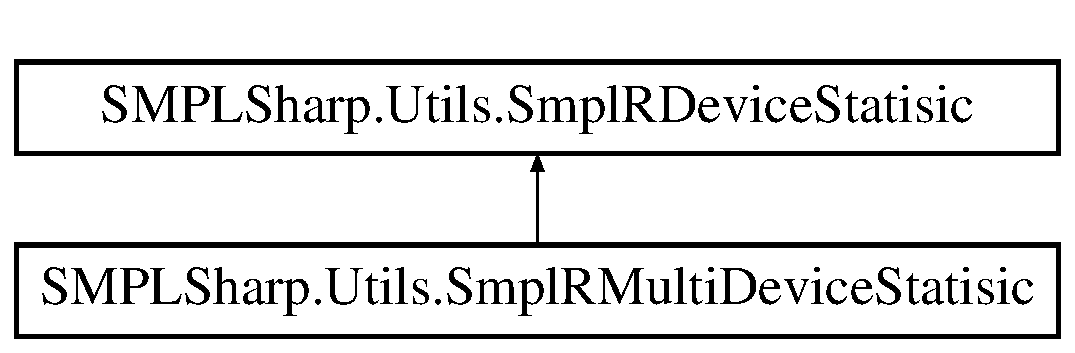
\includegraphics[height=2.000000cm]{d7/d3b/class_s_m_p_l_sharp_1_1_utils_1_1_smpl_r_device_statisic}
\end{center}
\end{figure}
\subsection*{Свойства}
\begin{DoxyCompactItemize}
\item 
string \hyperlink{class_s_m_p_l_sharp_1_1_utils_1_1_smpl_r_device_statisic_a7a9601632b7585ab8df008cd59698f0d}{Name}\hspace{0.3cm}{\ttfamily  \mbox{[}get, set\mbox{]}}
\begin{DoxyCompactList}\small\item\em Имя \end{DoxyCompactList}\item 
double \hyperlink{class_s_m_p_l_sharp_1_1_utils_1_1_smpl_r_device_statisic_aefc83dcc8f91247e91d1966ada1d7885}{Average\-Time\-Reserved}\hspace{0.3cm}{\ttfamily  \mbox{[}get, set\mbox{]}}
\begin{DoxyCompactList}\small\item\em Среднее время обслуживания заявки \end{DoxyCompactList}\item 
double \hyperlink{class_s_m_p_l_sharp_1_1_utils_1_1_smpl_r_device_statisic_a437aa023cf628ea90f8a0f7091fb7e27}{Busy\-Index}\hspace{0.3cm}{\ttfamily  \mbox{[}get, set\mbox{]}}
\begin{DoxyCompactList}\small\item\em Занятость прибора (0..1) \end{DoxyCompactList}\item 
int \hyperlink{class_s_m_p_l_sharp_1_1_utils_1_1_smpl_r_device_statisic_ac8c73d6bf105ba2983b1160b4b037cef}{Query\-Count}\hspace{0.3cm}{\ttfamily  \mbox{[}get, set\mbox{]}}
\begin{DoxyCompactList}\small\item\em Количество обслужанных заявок \end{DoxyCompactList}\end{DoxyCompactItemize}


\subsection{Подробное описание}
Статистика по прибору 



\subsection{Полный список свойств}
\hypertarget{class_s_m_p_l_sharp_1_1_utils_1_1_smpl_r_device_statisic_aefc83dcc8f91247e91d1966ada1d7885}{\index{S\-M\-P\-L\-Sharp\-::\-Utils\-::\-Smpl\-R\-Device\-Statisic@{S\-M\-P\-L\-Sharp\-::\-Utils\-::\-Smpl\-R\-Device\-Statisic}!Average\-Time\-Reserved@{Average\-Time\-Reserved}}
\index{Average\-Time\-Reserved@{Average\-Time\-Reserved}!SMPLSharp::Utils::SmplRDeviceStatisic@{S\-M\-P\-L\-Sharp\-::\-Utils\-::\-Smpl\-R\-Device\-Statisic}}
\subsubsection[{Average\-Time\-Reserved}]{\setlength{\rightskip}{0pt plus 5cm}double S\-M\-P\-L\-Sharp.\-Utils.\-Smpl\-R\-Device\-Statisic.\-Average\-Time\-Reserved\hspace{0.3cm}{\ttfamily [get]}, {\ttfamily [set]}}}\label{d7/d3b/class_s_m_p_l_sharp_1_1_utils_1_1_smpl_r_device_statisic_aefc83dcc8f91247e91d1966ada1d7885}


Среднее время обслуживания заявки 

\hypertarget{class_s_m_p_l_sharp_1_1_utils_1_1_smpl_r_device_statisic_a437aa023cf628ea90f8a0f7091fb7e27}{\index{S\-M\-P\-L\-Sharp\-::\-Utils\-::\-Smpl\-R\-Device\-Statisic@{S\-M\-P\-L\-Sharp\-::\-Utils\-::\-Smpl\-R\-Device\-Statisic}!Busy\-Index@{Busy\-Index}}
\index{Busy\-Index@{Busy\-Index}!SMPLSharp::Utils::SmplRDeviceStatisic@{S\-M\-P\-L\-Sharp\-::\-Utils\-::\-Smpl\-R\-Device\-Statisic}}
\subsubsection[{Busy\-Index}]{\setlength{\rightskip}{0pt plus 5cm}double S\-M\-P\-L\-Sharp.\-Utils.\-Smpl\-R\-Device\-Statisic.\-Busy\-Index\hspace{0.3cm}{\ttfamily [get]}, {\ttfamily [set]}}}\label{d7/d3b/class_s_m_p_l_sharp_1_1_utils_1_1_smpl_r_device_statisic_a437aa023cf628ea90f8a0f7091fb7e27}


Занятость прибора (0..1) 

\hypertarget{class_s_m_p_l_sharp_1_1_utils_1_1_smpl_r_device_statisic_a7a9601632b7585ab8df008cd59698f0d}{\index{S\-M\-P\-L\-Sharp\-::\-Utils\-::\-Smpl\-R\-Device\-Statisic@{S\-M\-P\-L\-Sharp\-::\-Utils\-::\-Smpl\-R\-Device\-Statisic}!Name@{Name}}
\index{Name@{Name}!SMPLSharp::Utils::SmplRDeviceStatisic@{S\-M\-P\-L\-Sharp\-::\-Utils\-::\-Smpl\-R\-Device\-Statisic}}
\subsubsection[{Name}]{\setlength{\rightskip}{0pt plus 5cm}string S\-M\-P\-L\-Sharp.\-Utils.\-Smpl\-R\-Device\-Statisic.\-Name\hspace{0.3cm}{\ttfamily [get]}, {\ttfamily [set]}}}\label{d7/d3b/class_s_m_p_l_sharp_1_1_utils_1_1_smpl_r_device_statisic_a7a9601632b7585ab8df008cd59698f0d}


Имя 

\hypertarget{class_s_m_p_l_sharp_1_1_utils_1_1_smpl_r_device_statisic_ac8c73d6bf105ba2983b1160b4b037cef}{\index{S\-M\-P\-L\-Sharp\-::\-Utils\-::\-Smpl\-R\-Device\-Statisic@{S\-M\-P\-L\-Sharp\-::\-Utils\-::\-Smpl\-R\-Device\-Statisic}!Query\-Count@{Query\-Count}}
\index{Query\-Count@{Query\-Count}!SMPLSharp::Utils::SmplRDeviceStatisic@{S\-M\-P\-L\-Sharp\-::\-Utils\-::\-Smpl\-R\-Device\-Statisic}}
\subsubsection[{Query\-Count}]{\setlength{\rightskip}{0pt plus 5cm}int S\-M\-P\-L\-Sharp.\-Utils.\-Smpl\-R\-Device\-Statisic.\-Query\-Count\hspace{0.3cm}{\ttfamily [get]}, {\ttfamily [set]}}}\label{d7/d3b/class_s_m_p_l_sharp_1_1_utils_1_1_smpl_r_device_statisic_ac8c73d6bf105ba2983b1160b4b037cef}


Количество обслужанных заявок 



Объявления и описания членов класса находятся в файле\-:\begin{DoxyCompactItemize}
\item 
D\-:/\-My Documents/\-Git\-Hub/\-S\-M\-P\-L\-Sharp/\-S\-M\-P\-L\-Sharp/Smpl\-Reporter.\-cs\end{DoxyCompactItemize}

\hypertarget{class_s_m_p_l_sharp_1_1_utils_1_1_smpl_reporter}{\section{Класс S\-M\-P\-L\-Sharp.\-Utils.\-Smpl\-Reporter}
\label{d2/d18/class_s_m_p_l_sharp_1_1_utils_1_1_smpl_reporter}\index{S\-M\-P\-L\-Sharp.\-Utils.\-Smpl\-Reporter@{S\-M\-P\-L\-Sharp.\-Utils.\-Smpl\-Reporter}}
}


Give model statistic  


\subsection*{Открытые члены}
\begin{DoxyCompactItemize}
\item 
\hyperlink{class_s_m_p_l_sharp_1_1_utils_1_1_smpl_reporter_ae6b7e1ab446c06fc292a459ae1719722}{Smpl\-Reporter} (\hyperlink{class_s_m_p_l_sharp_1_1_smpl_model}{Smpl\-Model} model)
\begin{DoxyCompactList}\small\item\em Конструктор для \hyperlink{class_s_m_p_l_sharp_1_1_utils_1_1_smpl_reporter}{Smpl\-Reporter} \end{DoxyCompactList}\end{DoxyCompactItemize}
\subsection*{Свойства}
\begin{DoxyCompactItemize}
\item 
int \hyperlink{class_s_m_p_l_sharp_1_1_utils_1_1_smpl_reporter_a0115cc791c67a57ba79083c12d4f163b}{Model\-Time}\hspace{0.3cm}{\ttfamily  \mbox{[}get\mbox{]}}
\begin{DoxyCompactList}\small\item\em Время моделирования \end{DoxyCompactList}\item 
List$<$ \hyperlink{class_s_m_p_l_sharp_1_1_utils_1_1_smpl_r_device_statisic}{Smpl\-R\-Device\-Statisic} $>$ \hyperlink{class_s_m_p_l_sharp_1_1_utils_1_1_smpl_reporter_ae368c8f35be0449aa5c5f52ddcc0ea0b}{Device\-Statistic}\hspace{0.3cm}{\ttfamily  \mbox{[}get\mbox{]}}
\begin{DoxyCompactList}\small\item\em Информация о приборах \end{DoxyCompactList}\item 
List$<$ \hyperlink{class_s_m_p_l_sharp_1_1_utils_1_1_smpl_r_multi_device_statisic}{Smpl\-R\-Multi\-Device\-Statisic} $>$ \hyperlink{class_s_m_p_l_sharp_1_1_utils_1_1_smpl_reporter_abef5661d7d82934362ad8504796b31af}{Multi\-Device\-Statistic}\hspace{0.3cm}{\ttfamily  \mbox{[}get\mbox{]}}
\begin{DoxyCompactList}\small\item\em Информация о многоканальных приборах \end{DoxyCompactList}\item 
List$<$ \hyperlink{class_s_m_p_l_sharp_1_1_utils_1_1_smpl_r_queue_statisic}{Smpl\-R\-Queue\-Statisic} $>$ \hyperlink{class_s_m_p_l_sharp_1_1_utils_1_1_smpl_reporter_a242251fbbe1facd190ed723f52285bfb}{Queue\-Statistic}\hspace{0.3cm}{\ttfamily  \mbox{[}get\mbox{]}}
\begin{DoxyCompactList}\small\item\em Информация о очередях \end{DoxyCompactList}\item 
\hyperlink{class_s_m_p_l_sharp_1_1_smpl_model}{Smpl\-Model} \hyperlink{class_s_m_p_l_sharp_1_1_utils_1_1_smpl_reporter_af01db9140661991e99d6978c250ff4c1}{Model}\hspace{0.3cm}{\ttfamily  \mbox{[}get, set\mbox{]}}
\begin{DoxyCompactList}\small\item\em Модель, с которой связан прибор \end{DoxyCompactList}\end{DoxyCompactItemize}


\subsection{Подробное описание}
Give model statistic 



\subsection{Конструктор(ы)}
\hypertarget{class_s_m_p_l_sharp_1_1_utils_1_1_smpl_reporter_ae6b7e1ab446c06fc292a459ae1719722}{\index{S\-M\-P\-L\-Sharp\-::\-Utils\-::\-Smpl\-Reporter@{S\-M\-P\-L\-Sharp\-::\-Utils\-::\-Smpl\-Reporter}!Smpl\-Reporter@{Smpl\-Reporter}}
\index{Smpl\-Reporter@{Smpl\-Reporter}!SMPLSharp::Utils::SmplReporter@{S\-M\-P\-L\-Sharp\-::\-Utils\-::\-Smpl\-Reporter}}
\subsubsection[{Smpl\-Reporter}]{\setlength{\rightskip}{0pt plus 5cm}S\-M\-P\-L\-Sharp.\-Utils.\-Smpl\-Reporter.\-Smpl\-Reporter (
\begin{DoxyParamCaption}
\item[{{\bf Smpl\-Model}}]{model}
\end{DoxyParamCaption}
)\hspace{0.3cm}{\ttfamily [inline]}}}\label{d2/d18/class_s_m_p_l_sharp_1_1_utils_1_1_smpl_reporter_ae6b7e1ab446c06fc292a459ae1719722}


Конструктор для \hyperlink{class_s_m_p_l_sharp_1_1_utils_1_1_smpl_reporter}{Smpl\-Reporter} 


\begin{DoxyParams}{Аргументы}
{\em model} & Модель\\
\hline
\end{DoxyParams}


\subsection{Полный список свойств}
\hypertarget{class_s_m_p_l_sharp_1_1_utils_1_1_smpl_reporter_ae368c8f35be0449aa5c5f52ddcc0ea0b}{\index{S\-M\-P\-L\-Sharp\-::\-Utils\-::\-Smpl\-Reporter@{S\-M\-P\-L\-Sharp\-::\-Utils\-::\-Smpl\-Reporter}!Device\-Statistic@{Device\-Statistic}}
\index{Device\-Statistic@{Device\-Statistic}!SMPLSharp::Utils::SmplReporter@{S\-M\-P\-L\-Sharp\-::\-Utils\-::\-Smpl\-Reporter}}
\subsubsection[{Device\-Statistic}]{\setlength{\rightskip}{0pt plus 5cm}List$<${\bf Smpl\-R\-Device\-Statisic}$>$ S\-M\-P\-L\-Sharp.\-Utils.\-Smpl\-Reporter.\-Device\-Statistic\hspace{0.3cm}{\ttfamily [get]}}}\label{d2/d18/class_s_m_p_l_sharp_1_1_utils_1_1_smpl_reporter_ae368c8f35be0449aa5c5f52ddcc0ea0b}


Информация о приборах 

\hypertarget{class_s_m_p_l_sharp_1_1_utils_1_1_smpl_reporter_af01db9140661991e99d6978c250ff4c1}{\index{S\-M\-P\-L\-Sharp\-::\-Utils\-::\-Smpl\-Reporter@{S\-M\-P\-L\-Sharp\-::\-Utils\-::\-Smpl\-Reporter}!Model@{Model}}
\index{Model@{Model}!SMPLSharp::Utils::SmplReporter@{S\-M\-P\-L\-Sharp\-::\-Utils\-::\-Smpl\-Reporter}}
\subsubsection[{Model}]{\setlength{\rightskip}{0pt plus 5cm}{\bf Smpl\-Model} S\-M\-P\-L\-Sharp.\-Utils.\-Smpl\-Reporter.\-Model\hspace{0.3cm}{\ttfamily [get]}, {\ttfamily [set]}}}\label{d2/d18/class_s_m_p_l_sharp_1_1_utils_1_1_smpl_reporter_af01db9140661991e99d6978c250ff4c1}


Модель, с которой связан прибор 

\hypertarget{class_s_m_p_l_sharp_1_1_utils_1_1_smpl_reporter_a0115cc791c67a57ba79083c12d4f163b}{\index{S\-M\-P\-L\-Sharp\-::\-Utils\-::\-Smpl\-Reporter@{S\-M\-P\-L\-Sharp\-::\-Utils\-::\-Smpl\-Reporter}!Model\-Time@{Model\-Time}}
\index{Model\-Time@{Model\-Time}!SMPLSharp::Utils::SmplReporter@{S\-M\-P\-L\-Sharp\-::\-Utils\-::\-Smpl\-Reporter}}
\subsubsection[{Model\-Time}]{\setlength{\rightskip}{0pt plus 5cm}int S\-M\-P\-L\-Sharp.\-Utils.\-Smpl\-Reporter.\-Model\-Time\hspace{0.3cm}{\ttfamily [get]}}}\label{d2/d18/class_s_m_p_l_sharp_1_1_utils_1_1_smpl_reporter_a0115cc791c67a57ba79083c12d4f163b}


Время моделирования 

\hypertarget{class_s_m_p_l_sharp_1_1_utils_1_1_smpl_reporter_abef5661d7d82934362ad8504796b31af}{\index{S\-M\-P\-L\-Sharp\-::\-Utils\-::\-Smpl\-Reporter@{S\-M\-P\-L\-Sharp\-::\-Utils\-::\-Smpl\-Reporter}!Multi\-Device\-Statistic@{Multi\-Device\-Statistic}}
\index{Multi\-Device\-Statistic@{Multi\-Device\-Statistic}!SMPLSharp::Utils::SmplReporter@{S\-M\-P\-L\-Sharp\-::\-Utils\-::\-Smpl\-Reporter}}
\subsubsection[{Multi\-Device\-Statistic}]{\setlength{\rightskip}{0pt plus 5cm}List$<${\bf Smpl\-R\-Multi\-Device\-Statisic}$>$ S\-M\-P\-L\-Sharp.\-Utils.\-Smpl\-Reporter.\-Multi\-Device\-Statistic\hspace{0.3cm}{\ttfamily [get]}}}\label{d2/d18/class_s_m_p_l_sharp_1_1_utils_1_1_smpl_reporter_abef5661d7d82934362ad8504796b31af}


Информация о многоканальных приборах 

\hypertarget{class_s_m_p_l_sharp_1_1_utils_1_1_smpl_reporter_a242251fbbe1facd190ed723f52285bfb}{\index{S\-M\-P\-L\-Sharp\-::\-Utils\-::\-Smpl\-Reporter@{S\-M\-P\-L\-Sharp\-::\-Utils\-::\-Smpl\-Reporter}!Queue\-Statistic@{Queue\-Statistic}}
\index{Queue\-Statistic@{Queue\-Statistic}!SMPLSharp::Utils::SmplReporter@{S\-M\-P\-L\-Sharp\-::\-Utils\-::\-Smpl\-Reporter}}
\subsubsection[{Queue\-Statistic}]{\setlength{\rightskip}{0pt plus 5cm}List$<${\bf Smpl\-R\-Queue\-Statisic}$>$ S\-M\-P\-L\-Sharp.\-Utils.\-Smpl\-Reporter.\-Queue\-Statistic\hspace{0.3cm}{\ttfamily [get]}}}\label{d2/d18/class_s_m_p_l_sharp_1_1_utils_1_1_smpl_reporter_a242251fbbe1facd190ed723f52285bfb}


Информация о очередях 



Объявления и описания членов класса находятся в файле\-:\begin{DoxyCompactItemize}
\item 
D\-:/\-My Documents/\-Git\-Hub/\-S\-M\-P\-L\-Sharp/\-S\-M\-P\-L\-Sharp/Smpl\-Reporter.\-cs\end{DoxyCompactItemize}

\hypertarget{class_s_m_p_l_sharp_1_1_utils_1_1_smpl_r_multi_device_statisic}{\section{Класс S\-M\-P\-L\-Sharp.\-Utils.\-Smpl\-R\-Multi\-Device\-Statisic}
\label{de/d2e/class_s_m_p_l_sharp_1_1_utils_1_1_smpl_r_multi_device_statisic}\index{S\-M\-P\-L\-Sharp.\-Utils.\-Smpl\-R\-Multi\-Device\-Statisic@{S\-M\-P\-L\-Sharp.\-Utils.\-Smpl\-R\-Multi\-Device\-Statisic}}
}


Статистика по многоканальному прибору  


Граф наследования\-:S\-M\-P\-L\-Sharp.\-Utils.\-Smpl\-R\-Multi\-Device\-Statisic\-:\begin{figure}[H]
\begin{center}
\leavevmode
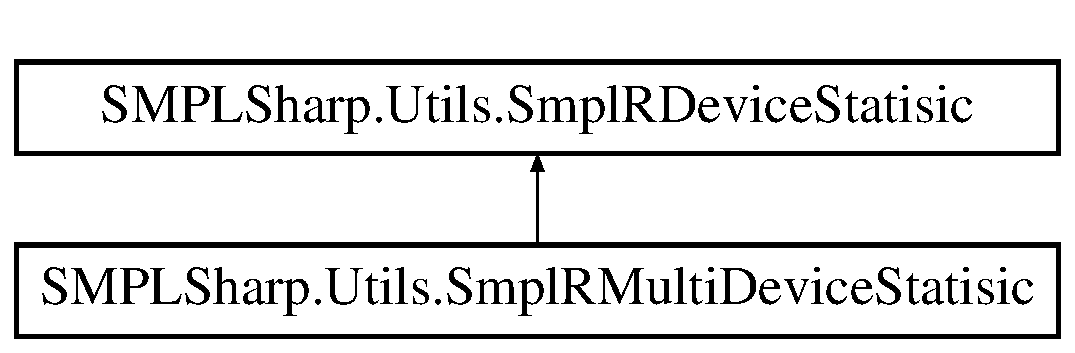
\includegraphics[height=2.000000cm]{de/d2e/class_s_m_p_l_sharp_1_1_utils_1_1_smpl_r_multi_device_statisic}
\end{center}
\end{figure}
\subsection*{Свойства}
\begin{DoxyCompactItemize}
\item 
int \hyperlink{class_s_m_p_l_sharp_1_1_utils_1_1_smpl_r_multi_device_statisic_a918293b0514cc2084174138c94f3a56c}{Channel\-Count}\hspace{0.3cm}{\ttfamily  \mbox{[}get, set\mbox{]}}
\begin{DoxyCompactList}\small\item\em Количество каналов \end{DoxyCompactList}\end{DoxyCompactItemize}


\subsection{Подробное описание}
Статистика по многоканальному прибору 



\subsection{Полный список свойств}
\hypertarget{class_s_m_p_l_sharp_1_1_utils_1_1_smpl_r_multi_device_statisic_a918293b0514cc2084174138c94f3a56c}{\index{S\-M\-P\-L\-Sharp\-::\-Utils\-::\-Smpl\-R\-Multi\-Device\-Statisic@{S\-M\-P\-L\-Sharp\-::\-Utils\-::\-Smpl\-R\-Multi\-Device\-Statisic}!Channel\-Count@{Channel\-Count}}
\index{Channel\-Count@{Channel\-Count}!SMPLSharp::Utils::SmplRMultiDeviceStatisic@{S\-M\-P\-L\-Sharp\-::\-Utils\-::\-Smpl\-R\-Multi\-Device\-Statisic}}
\subsubsection[{Channel\-Count}]{\setlength{\rightskip}{0pt plus 5cm}int S\-M\-P\-L\-Sharp.\-Utils.\-Smpl\-R\-Multi\-Device\-Statisic.\-Channel\-Count\hspace{0.3cm}{\ttfamily [get]}, {\ttfamily [set]}}}\label{de/d2e/class_s_m_p_l_sharp_1_1_utils_1_1_smpl_r_multi_device_statisic_a918293b0514cc2084174138c94f3a56c}


Количество каналов 



Объявления и описания членов класса находятся в файле\-:\begin{DoxyCompactItemize}
\item 
D\-:/\-My Documents/\-Git\-Hub/\-S\-M\-P\-L\-Sharp/\-S\-M\-P\-L\-Sharp/Smpl\-Reporter.\-cs\end{DoxyCompactItemize}

\hypertarget{class_s_m_p_l_sharp_1_1_utils_1_1_smpl_r_queue_statisic}{\section{Класс S\-M\-P\-L\-Sharp.\-Utils.\-Smpl\-R\-Queue\-Statisic}
\label{de/de9/class_s_m_p_l_sharp_1_1_utils_1_1_smpl_r_queue_statisic}\index{S\-M\-P\-L\-Sharp.\-Utils.\-Smpl\-R\-Queue\-Statisic@{S\-M\-P\-L\-Sharp.\-Utils.\-Smpl\-R\-Queue\-Statisic}}
}


Статистика по очереди  


\subsection*{Свойства}
\begin{DoxyCompactItemize}
\item 
string \hyperlink{class_s_m_p_l_sharp_1_1_utils_1_1_smpl_r_queue_statisic_aaa07c8c4d4ff07e2cb102dcadc700860}{Name}\hspace{0.3cm}{\ttfamily  \mbox{[}get, set\mbox{]}}
\begin{DoxyCompactList}\small\item\em Имя \end{DoxyCompactList}\item 
double \hyperlink{class_s_m_p_l_sharp_1_1_utils_1_1_smpl_r_queue_statisic_a219830367adab4aac8538c90ebfba282}{Average\-Time\-Waiting}\hspace{0.3cm}{\ttfamily  \mbox{[}get, set\mbox{]}}
\begin{DoxyCompactList}\small\item\em Среднее время ожидания \end{DoxyCompactList}\item 
double \hyperlink{class_s_m_p_l_sharp_1_1_utils_1_1_smpl_r_queue_statisic_ac39d2d7f7417cccfb3f7c8e8ccbb34e6}{Dispersal\-Time\-Waiting}\hspace{0.3cm}{\ttfamily  \mbox{[}get, set\mbox{]}}
\begin{DoxyCompactList}\small\item\em Разброс времени ожидания \end{DoxyCompactList}\item 
double \hyperlink{class_s_m_p_l_sharp_1_1_utils_1_1_smpl_r_queue_statisic_aab2840b938ed22bd81799f7882cbc6e1}{Average\-Length}\hspace{0.3cm}{\ttfamily  \mbox{[}get, set\mbox{]}}
\begin{DoxyCompactList}\small\item\em Средняя длина очереди \end{DoxyCompactList}\item 
int \hyperlink{class_s_m_p_l_sharp_1_1_utils_1_1_smpl_r_queue_statisic_af0c96a5114802513777f2d4cf5e176b9}{Max\-Length}\hspace{0.3cm}{\ttfamily  \mbox{[}get, set\mbox{]}}
\begin{DoxyCompactList}\small\item\em Максимальная длина очереди \end{DoxyCompactList}\item 
int \hyperlink{class_s_m_p_l_sharp_1_1_utils_1_1_smpl_r_queue_statisic_aba57ab69353bec5cd8415a53bd6644fe}{Total\-Count}\hspace{0.3cm}{\ttfamily  \mbox{[}get, set\mbox{]}}
\begin{DoxyCompactList}\small\item\em Число заявок, попавших в очередь \end{DoxyCompactList}\end{DoxyCompactItemize}


\subsection{Подробное описание}
Статистика по очереди 



См. определение в файле Smpl\-Reporter.\-cs строка 90



\subsection{Полный список свойств}
\hypertarget{class_s_m_p_l_sharp_1_1_utils_1_1_smpl_r_queue_statisic_aab2840b938ed22bd81799f7882cbc6e1}{\index{S\-M\-P\-L\-Sharp\-::\-Utils\-::\-Smpl\-R\-Queue\-Statisic@{S\-M\-P\-L\-Sharp\-::\-Utils\-::\-Smpl\-R\-Queue\-Statisic}!Average\-Length@{Average\-Length}}
\index{Average\-Length@{Average\-Length}!SMPLSharp::Utils::SmplRQueueStatisic@{S\-M\-P\-L\-Sharp\-::\-Utils\-::\-Smpl\-R\-Queue\-Statisic}}
\subsubsection[{Average\-Length}]{\setlength{\rightskip}{0pt plus 5cm}double S\-M\-P\-L\-Sharp.\-Utils.\-Smpl\-R\-Queue\-Statisic.\-Average\-Length\hspace{0.3cm}{\ttfamily [get]}, {\ttfamily [set]}}}\label{de/de9/class_s_m_p_l_sharp_1_1_utils_1_1_smpl_r_queue_statisic_aab2840b938ed22bd81799f7882cbc6e1}


Средняя длина очереди 



См. определение в файле Smpl\-Reporter.\-cs строка 129

\hypertarget{class_s_m_p_l_sharp_1_1_utils_1_1_smpl_r_queue_statisic_a219830367adab4aac8538c90ebfba282}{\index{S\-M\-P\-L\-Sharp\-::\-Utils\-::\-Smpl\-R\-Queue\-Statisic@{S\-M\-P\-L\-Sharp\-::\-Utils\-::\-Smpl\-R\-Queue\-Statisic}!Average\-Time\-Waiting@{Average\-Time\-Waiting}}
\index{Average\-Time\-Waiting@{Average\-Time\-Waiting}!SMPLSharp::Utils::SmplRQueueStatisic@{S\-M\-P\-L\-Sharp\-::\-Utils\-::\-Smpl\-R\-Queue\-Statisic}}
\subsubsection[{Average\-Time\-Waiting}]{\setlength{\rightskip}{0pt plus 5cm}double S\-M\-P\-L\-Sharp.\-Utils.\-Smpl\-R\-Queue\-Statisic.\-Average\-Time\-Waiting\hspace{0.3cm}{\ttfamily [get]}, {\ttfamily [set]}}}\label{de/de9/class_s_m_p_l_sharp_1_1_utils_1_1_smpl_r_queue_statisic_a219830367adab4aac8538c90ebfba282}


Среднее время ожидания 



См. определение в файле Smpl\-Reporter.\-cs строка 109

\hypertarget{class_s_m_p_l_sharp_1_1_utils_1_1_smpl_r_queue_statisic_ac39d2d7f7417cccfb3f7c8e8ccbb34e6}{\index{S\-M\-P\-L\-Sharp\-::\-Utils\-::\-Smpl\-R\-Queue\-Statisic@{S\-M\-P\-L\-Sharp\-::\-Utils\-::\-Smpl\-R\-Queue\-Statisic}!Dispersal\-Time\-Waiting@{Dispersal\-Time\-Waiting}}
\index{Dispersal\-Time\-Waiting@{Dispersal\-Time\-Waiting}!SMPLSharp::Utils::SmplRQueueStatisic@{S\-M\-P\-L\-Sharp\-::\-Utils\-::\-Smpl\-R\-Queue\-Statisic}}
\subsubsection[{Dispersal\-Time\-Waiting}]{\setlength{\rightskip}{0pt plus 5cm}double S\-M\-P\-L\-Sharp.\-Utils.\-Smpl\-R\-Queue\-Statisic.\-Dispersal\-Time\-Waiting\hspace{0.3cm}{\ttfamily [get]}, {\ttfamily [set]}}}\label{de/de9/class_s_m_p_l_sharp_1_1_utils_1_1_smpl_r_queue_statisic_ac39d2d7f7417cccfb3f7c8e8ccbb34e6}


Разброс времени ожидания 



См. определение в файле Smpl\-Reporter.\-cs строка 119

\hypertarget{class_s_m_p_l_sharp_1_1_utils_1_1_smpl_r_queue_statisic_af0c96a5114802513777f2d4cf5e176b9}{\index{S\-M\-P\-L\-Sharp\-::\-Utils\-::\-Smpl\-R\-Queue\-Statisic@{S\-M\-P\-L\-Sharp\-::\-Utils\-::\-Smpl\-R\-Queue\-Statisic}!Max\-Length@{Max\-Length}}
\index{Max\-Length@{Max\-Length}!SMPLSharp::Utils::SmplRQueueStatisic@{S\-M\-P\-L\-Sharp\-::\-Utils\-::\-Smpl\-R\-Queue\-Statisic}}
\subsubsection[{Max\-Length}]{\setlength{\rightskip}{0pt plus 5cm}int S\-M\-P\-L\-Sharp.\-Utils.\-Smpl\-R\-Queue\-Statisic.\-Max\-Length\hspace{0.3cm}{\ttfamily [get]}, {\ttfamily [set]}}}\label{de/de9/class_s_m_p_l_sharp_1_1_utils_1_1_smpl_r_queue_statisic_af0c96a5114802513777f2d4cf5e176b9}


Максимальная длина очереди 



См. определение в файле Smpl\-Reporter.\-cs строка 139

\hypertarget{class_s_m_p_l_sharp_1_1_utils_1_1_smpl_r_queue_statisic_aaa07c8c4d4ff07e2cb102dcadc700860}{\index{S\-M\-P\-L\-Sharp\-::\-Utils\-::\-Smpl\-R\-Queue\-Statisic@{S\-M\-P\-L\-Sharp\-::\-Utils\-::\-Smpl\-R\-Queue\-Statisic}!Name@{Name}}
\index{Name@{Name}!SMPLSharp::Utils::SmplRQueueStatisic@{S\-M\-P\-L\-Sharp\-::\-Utils\-::\-Smpl\-R\-Queue\-Statisic}}
\subsubsection[{Name}]{\setlength{\rightskip}{0pt plus 5cm}string S\-M\-P\-L\-Sharp.\-Utils.\-Smpl\-R\-Queue\-Statisic.\-Name\hspace{0.3cm}{\ttfamily [get]}, {\ttfamily [set]}}}\label{de/de9/class_s_m_p_l_sharp_1_1_utils_1_1_smpl_r_queue_statisic_aaa07c8c4d4ff07e2cb102dcadc700860}


Имя 



См. определение в файле Smpl\-Reporter.\-cs строка 99

\hypertarget{class_s_m_p_l_sharp_1_1_utils_1_1_smpl_r_queue_statisic_aba57ab69353bec5cd8415a53bd6644fe}{\index{S\-M\-P\-L\-Sharp\-::\-Utils\-::\-Smpl\-R\-Queue\-Statisic@{S\-M\-P\-L\-Sharp\-::\-Utils\-::\-Smpl\-R\-Queue\-Statisic}!Total\-Count@{Total\-Count}}
\index{Total\-Count@{Total\-Count}!SMPLSharp::Utils::SmplRQueueStatisic@{S\-M\-P\-L\-Sharp\-::\-Utils\-::\-Smpl\-R\-Queue\-Statisic}}
\subsubsection[{Total\-Count}]{\setlength{\rightskip}{0pt plus 5cm}int S\-M\-P\-L\-Sharp.\-Utils.\-Smpl\-R\-Queue\-Statisic.\-Total\-Count\hspace{0.3cm}{\ttfamily [get]}, {\ttfamily [set]}}}\label{de/de9/class_s_m_p_l_sharp_1_1_utils_1_1_smpl_r_queue_statisic_aba57ab69353bec5cd8415a53bd6644fe}


Число заявок, попавших в очередь 



См. определение в файле Smpl\-Reporter.\-cs строка 150



Объявления и описания членов класса находятся в файле\-:\begin{DoxyCompactItemize}
\item 
D\-:/\-My Documents/\-Git\-Hub/\-S\-M\-P\-L\-Sharp/\-S\-M\-P\-L\-Sharp/Smpl\-Reporter.\-cs\end{DoxyCompactItemize}

\addcontentsline{toc}{part}{Алфавитный указатель}
\printindex
\end{document}
